\documentclass[12pt,a4paper,ngerman]{report}
\usepackage{babel}
\usepackage{graphicx}
\usepackage[utf8]{inputenc}

%\usepackage{float}
\usepackage{floatflt}
\usepackage{wrapfig}

\author{Roman Scherer \\ scherer@informatik.hu-berlin.de}

\title{{\small
    Humboldt-Universität zu Berlin \\
    Mathematisch-Naturwissenschaftliche Fakultät II \\
    Institut für Informatik \\
    Lehrstuhl für Systemarchitektur \\
    Unter den Linden 6 \\
    D-10099 Berlin \\
  } \vspace{0.4cm}
  
\includegraphics[width=4cm]{bilder/husiegel_bw} \\
  \vspace{0.4cm}
  \large{Diplomarbeit} \\
  \LARGE{\textbf{Konzeption und Implementierung einer Community-Plattform für Surfer}} \\
}


\begin{document}

\maketitle


\begin{abstract}
  Surfen oder Wellenreiten ist eine Wassersportart, die besonders
  stark vom Wetter, den Gezeiten und den Eigenschaften der zu
  surfenden Wellen abhängig ist. Im Rahmen dieser Diplomarbeit soll
  eine \textit{Community-Plattform} für das Internet entwickelt
  werden, auf der Surfer für sie wichtige Informationen finden und
  austauschen können. Die bei der Konzeption und Implementierung
  auftretenden Probleme und Lösungen sollen in dieser Arbeit
  diskutiert werden.
\end{abstract}

%%% Local Variables:
%%% mode: latex
%%% TeX-master: "../community-plattform"
%%% End:


\tableofcontents


\chapter{Einleitung}

\section{Motivation}

Mit Surfen oder Wellenreiten bezeichnet man eine Wassersportart, bei
der versucht wird, auf einem Surfbrett stehend eine brechende Welle
entlang zu fahren. Anders als beim Windsurfen wird hier nicht die
Kraft des Windes, sondern die Kraft der brechenden Welle benutzt, um
die zum Aufstehen und Fahren benötigte Geschwindigkeit zu
erreichen. Zum Surfen geeignete Wellen fangen idealerweise an einem
Punkt an zu brechen, und fallen dann kontinuierlich in eine oder beide
Richtungen in sich zusammen. Der Surfer versucht die Welle am
brechenden Punkt anzupaddeln, aufzustehen um dann auf der Welle so
lange wie möglich in die brechende Richtung zu fahren.

Diese Wellen sind allerdings nicht immer dort anzutreffen wo es ein
Meer oder einen Strand gibt. Vielmehr sind für Surfer interessante
Wellen an den Orten zu finden, im folgenden \textit{Spots} genannt,
deren geografische Lage das Eintreffen von oft weit entfernt
entstandenen Wellen begünstigt. Die Beschaffenheit des Untergrunds,
über dem die Wellen brechen, ist außerdem ein wichtiger Faktor, der
die Qualität der zu surfenden Wellen beeinflusst. An den bei Surfern
sehr beliebten \textit{Pointbreaks} brechen die Wellen immer an einem
bestimmten Punkt über einem Riff oder steinigem Boden. Diese sind die
beständigsten, am besten einschätzbaren, aber auch gefährlichsten
Spots.

Besteht der Untergrund aus Sand, sind meist durch Gezeiten, Strömungen
und Stürme sich ständig verändernde Sandbänke für das Brechen der
Wellen verantwortlich. Weitere wichtige Faktoren, die sich auf die
Eigenschaften von surfbaren Wellen auswirken, sind die Gezeiten, die
Richtung aus der die Wellen kommen, sowie die Wind- und
Wetterverhältnisse in den jeweiligen Jahreszeiten.

Die sogenannten \textit{Stormrider Guides} des \textit{Low Pressure}
Verlags sind seit langem die populärsten Reiseführer in der
Surfszene. Sie erfreuen sich dank der vielen hilfreichen Informationen
und Tipps einer sehr großen Beliebtheit. Die nach Kontinenten und
Ländern gegliederten Bücher enthalten Reiseinformationen über Land und
Leute, Kultur, Klima sowie Kartenausschnitte mit Beschreibungen zu den
Surfbedingungen, die an den jeweiligen Spots herrschen. Insbesondere
die detaillierten Informationen über die Eigenschaften der Wellen und
der Umgebung sind von großem Nutzen. Zum Beispiel wird beschrieben zu
welcher Gezeit bzw. \textit{Tide} die Wellen an einem Spot am besten brechen,
wie stark die Meeresströmung ist oder ob die Brandung an einem
Sandstrand oder auf einem flachen Riff ist.

% \begin{figure}[h]
%   \begin{center}
%     \includegraphics[width=450px]{bilder/stormrider-sample}
%     \caption{Beispiel aus dem World Stormrider Guide}
%   \end{center}
% \end{figure}

\section{Swell - Die Entstehung von Wellen}
Die besten Surfspots auf der Welt sind meist in den Ländern zu finden,
in denen regelmäßig \textit{Swell} eintrifft. Mit \textit{Swell} oder
\textit{Dünung} werden Seewellen bezeichnet, deren Entstehungs\-gebiet
weit entfernt ist von dem Ort an dem sie eintreffen und brechen. Swell
wird von den unterschiedlichsten Wetter\-phänomenen, wie
z.B. Wirbelstürmen, Passatwinden, Monsune und Tiefdruckgebieten
erzeugt \cite[S.15]{storm_europe_1998}. In Europa eintreffender Swell
entsteht hauptsächlich durch die Luftzirkulation in Tiefdruckgebieten
auf dem Atlantik.

\begin{figure}[h]
  \begin{center}
    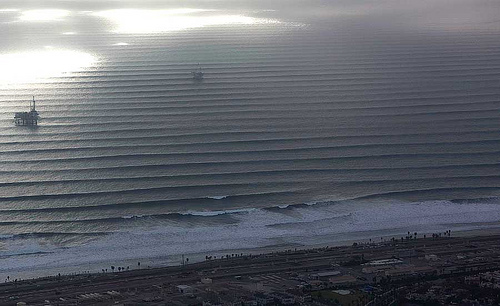
\includegraphics{bilder/swell}
    \caption{Linienförmig eintreffender Swell}
  \end{center}
\end{figure}

Wellen entstehen dadurch, dass die Wasseroberfläche durch die über ihr
strömenden Winde in Bewegung versetzt wird. Die Gipfel und Täler der
Wellen werden durch die Zirkulation des Windes über der Oberfläche
immer höher und tiefer, bis sie ein Limit erreichen und wieder in sich
zusammenbrechen. Die Höhe der Wellen ist dabei von der Stärke, der
Dauer und der Lauflänge \footnote{die Strecke über der Wind strömt}
des Windes abhängig.

Die so erzeugten Wellen breiten sich dann vom Entstehungsort
kreisförmig auf ihre Umgebung im Meer aus. Die Geschwindigkeit ist
dabei abhängig von der \textit{Wellenlänge}, dem Abstand zwischen zwei
Wellengipfeln. Das Wellenchaos am Entstehungsort mit vielen
unterschiedlichen Wellenlängen beginnt sich mit der Ausbreitung zu
legen. Die schnelleren Wellen, mit weiter auseinander liegenden
Gipfeln, beginnen die langsameren Wellen zu überholen und fangen an
sich linienförmig zu ordnen. Die vorderen Wellen werden dabei zu den
kräftiger und sauber angeordneten, die hinteren Wellen zu den
schwächeren und chaotischeren. Je weiter die Strecke die ein Swell
hinter sich gelegt hat und linienförmiger er geordnet ist, desto
größer ist die Geschwindigkeit und die Kraft der Wellen am Ort an dem
sie brechen.

Swell ist eine der Grundvoraussetzungen für gute und surfbare
Wellen. Deshalb gibt es z.B. auch in Deutschland keine guten
Surfspots, da der potentiell eintreffende Swell meistens durch England
abgeschirmt wird.

\section{Voraussetzungen zum Surfen}

\section{Ziel der Diplomarbeit}

Ziel der Diplomarbeit ist die Entwicklung einer \textit{Community
  Plattform} für Surfer, welche den Grundgedanken der
\textit{Stormrider Guides} aufgreift, mit den neuen Möglichkeiten des
Internets und des Web 2.0 verknüpft, und somit einen Mehrwert für
Surfer generiert. Grundlage der Plattform sollen Beschreibungen und
Kommentare der Mitglieder zu den verschiedenen Surf Spots sein. Diese
werden dann mit anderen Diensten wie \textit{Google Maps},
\textit{Flickr} und \textit{YouTube} verknüpft. Außerdem sollen
Wetter- und Wellenvorhersagen für die verschiedenen Spots integriert
werden, um aktuelle Informationen zu den Surfbedingungen
bereitzustellen.

Die bei der Konzeption und Implementierung aufgetretenen Probleme und
Lösungen werden in dieser Arbeit vorgestellt.



% 
{\sf \footnotesize
  \begin{tabular}{|p{2.5cm}p{0.7cm}p{0.7cm}|}
    \hline
    & & \\
    \multicolumn{3}{|l|}{\textbf{Hai Angriff Statistik}} \\
    \multicolumn{3}{|l|}{für Länder mit mehr als 10 Angriffen} \\
    & & \\
    & \textbf{Tota}l & \textbf{Fatal} \\
    \textbf{Europa} & \textbf{38} & \textbf{18} \\
    Italien & 14 & 4 \\
    \textbf{Afrika} & \textbf{255} & \textbf{67} \\
    Südafrika & 208 & 41 \\
    Mosambik & 11 & 3 \\
    \textbf{Indischer Ozean} & \textbf{62} & \textbf{27} \\
    Maskarenen & 21 & 12 \\
    Iran & 23 & 8 \\
    Indien & 10 & 4 \\
    \textbf{Ost Asien} & \textbf{89} & \textbf{38} \\
    Papua-Neuguinea & 36 & 15 \\
    Philippinen & 15 & 6 \\
    Japan & 19 & 12 \\
    \textbf{Australien \& Neuseeland} & \textbf{326} & \textbf{141} \\
    West Australien & 28 & 9 \\
    Süd Australien & 30 & 16 \\
    Victoria & 20 & 8 \\
    Tasmanien & 16 & 6 \\
    Neusüdwales & 123 & 62 \\
    Queensland & 101 & 47 \\
    \textbf{Pazifik} & \textbf{211} & \textbf{62} \\
    Marshallinseln & 12 & 0 \\
    Salomon-Inseln & 17 & 8 \\
    Fiji & 25 & 10 \\
    Hawaii & 104 & 19 \\
    \textbf{Nord Amerika} & \textbf{720} & \textbf{38} \\
    Oregon & 17 & 1 \\
    Kalifornien & 111 & 8 \\
    Texas & 30 & 3 \\
    Florida & 187 & 13 \\
    Südkarolina & 43 & 3 \\
    Nordkarolina & 24 & 3 \\
    New Jersey & 16 & 5 \\
    \textbf{Zentralamerika} & \textbf{118} & \textbf{50} \\
    Mexiko & 39 & 21 \\
    Panama & 16 & 9 \\
    \textbf{Südamerika} & \textbf{89} & \textbf{21} \\
    Brasilien & 81 & 20 \\
    & & \\
    \textbf{TOTAL} & \textbf{1909} & \textbf{456} \\
    & & \\
    \multicolumn{3}{|l|}{The International Shark Attack File,} \\
    \multicolumn{3}{|l|}{Florida Museum of Natural History,} \\
    \multicolumn{3}{|l|}{University of Florida.} \\
%    \multicolumn{3}{|l|}{{\tiny http://www.flmnh.ufl.edu/fish/Sharks/ISAF/ISAF.htm}} \\
    \hline
  \end{tabular}
}

%%% Local Variables:
%%% mode: latex
%%% TeX-master: "../community-plattform"
%%% End:


%%% Local Variables:
%%% mode: latex
%%% TeX-master: "../community-plattform"
%%% End:


\chapter{Anforderungen an die Web Applikation}

\section{Spot Beschreibungen}

Eine der bekanntesten Wellen in Europa ist im spanischen Baskenland an
einer Fluss\-mündung östlich des Ortes \textit{Mundaka} zu finden. Im
\textit{Stormrider Guide Europe} \cite[S.180]{storm_europe_1998}
werden die Surfbedingungen an diesem Spot wie folgt beschrieben.

\textit{Some of the longest, hollowest lefts in Europe break over
  sandbanks at the mouth of the river Gernike. It's best at low tide,
  when the rivers current (a useful conveyor belt) is less intense,
  and holds swell up to 4m (12ft). On the other side of the rivermouth
  are the beaches Laida and Laga where you can find waves at small
  swells. The river and its estuary are a Worldwide Fund for Nature
  reserve, but even so, the water is not as clean as could expected.
}

Zusätzlich werden den Beschreibungen Piktogramme aus verschiedenen
Kategorien zugeordnet, welche die Gegebenheiten vor Ort durch eine
vereinfachte grafische Darstellung widerspiegeln. Einige dieser
Kategorien sind die bevorzugte Windrichtung, die optimale Gezeit, die
Art der brechenden Welle, Beschaffenheit des Bodens, sowie mögliche
Gefahren. Kennt man einmal die Piktogramme, ist durch einen kurzen
Blick schnell ersichtlich welche Bedingungen an einem Spot herrschen.

\begin{figure}[h]
  \begin{center}
    
\includegraphics[height=40px]{bilder/mundaka-conditions}
    \caption{Piktogramme zu den Surfbedingungen in Mundaka}
    \label{piktogramm}
  \end{center}
\end{figure}


In Abbildung \ref{piktogramm} sind die Piktogramme zu sehen, die für
die obige Beschreibung in Mundaka verwendet wurden. Sie sollen
vermitteln, dass dieser Spot sehr bekannt ist und an guten Tagen mit
vielen Surfern zu rechnen ist. Die Welle bricht mit viel Kraft von
links nach rechts (\textit{Left-hander}, immer vom Strand aus gesehen)
über einer Sandbank, wobei vereinzelt Surfbretter zu Bruch gehen
können.  Sie ist nicht bei Flut (\textit{High Tide}) surfbar, und
ablandiger Wind (\textit{Offshore}) aus dem Süden trägt dazu bei, dass
die Wellen geglättet werden, später brechen und hohler werden.

Das Konzept der Stormrider Guides soll die Grundlage der Web
Applikation bilden und mit den neuen Möglichkeiten des Internets
verknüpft werden. Die Beschreibungen zu den Spots und deren
Gegebenheiten sollen gemeinschaflich durch die Mitglieder der Surf
Community verfasst werden, und als sogenannter \textit{User Generated
  Content} verwaltet werden. Die gemeinsam erstellten Beschreibungen
sollen eine objektive Sicht auf die Gegebenheiten und Surfbedingungen
an den jeweiligen Spots bieten. Für persönliche Ansichten und
Diskussionen sollen Kommentarfunktionen zur Verfügung gestellt werden
die in Abschnitt \ref{subsec:Kommentare} beschrieben werden.

Um Spam und anderer mutwilliger Zerstörung oder Verunreinigung des
Contents vorzubeugen ist eine Registrierung der Nutzer
erforderlich. Für alle Informationen die zu einem Spot gehören und von
Nutzern der Web Applikation verändert werden können, soll eine
Historie verwaltet werden. Dies soll sicherstellen, dass bei einer
eventuellen Veruneinigung des Contents auf eine frührere Version der
Information zurückgegriffen, und diese wiederhergestellt werden kann.

\section{Kartenmaterial}

Um das Auffinden von Spots zu vereinfachen sollen diese auf einer
Karte dargestellt werden. Webservice Dienste wie \textit{Google Maps},
\textit{Yahoo! Maps} oder Microsoft's \textit{Bing Maps}
\footnote{seit Juni 2009, früher: Microsoft's Virtual Earth} bieten
die Möglichkeit interaktive Karten per Java\-script oder Flash in eine
Webseite einzubetten. Diese Dienste bieten nicht nur die typischen
Land- bzw. Straßenkarten an, sondern stellen auch Satelitenbilder und
teilweise 3-dimensionale Ansichten für bestimmte Gebiete zur
Verfügung.

\section{Wetter- und Wellendaten}
\label{sec:Wetter- und Wellendaten}

Wie schon in der Einleitung erwähnt ist das Vorhandensein von Swell
eine der Grundvoraussetzungen zum Surfen. Viele Surfer nutzen deshalb
regelmäßig Dienste im Internet um sich über die Wetter- und
Wellenverhältnisse in den nächsten Tagen zu informieren. Dabei ist
hauptsächlich die Wellenhöhe, die Wellenperiode und die Stärke und
Richtung des Windes von Interesse. Die Spot Beschreibungen sollen
deshalb mit aktuellen Wetter- und Wellenvorhersagen verknüpft werden,
um den Benutzern der Web Applikation einen Mehrwert zu bieten. Die
\textit{National Oceanic and Atmospheric Administration (NOAA)} ist
die Wetter- und Ozeanografiebehörde der Vereinigten Staaten. Sie
besteht aus 5 größeren Organisationen, zu denen unter anderen auch der
\textit{National Weather Service} und der \textit{National Ocean
  Service} gehören, welche die benötigten Wetter- und Wellendaten zur
Verfügung stellen. Viele der im Internet verfügbaren Dienste, die
Wetter- oder Wellenvorhersagen anbieten, beziehen ihre Daten ebenfalls
von diesen Organisationen.

\section{Bilder \& Videos}

Um Surfern einen visuellen Eindruck von einem Spot zu bieten, sollen
die Spots mit Bildern und Videos verknüpft und somit aufgewertet
werden. Auf Internetseiten wie \textit{Flickr} und \textit{YouTube}
sind von vielen bekannten Spots Bilder und Videos zu finden. Eine
Suchanfrage nach einem der bekanntesten Spots mit den Stichwörtern
\textit{Mavericks} und \textit{Surf} ergab im Juni 2009 bei
\textit{Flickr} 2319 und bei \textit{YouTube} 548 Ergebnisse. Diese in
der Surf Community gerne gesehenen Bilder und Videos sind ideal um das
bisher aus Beschreibungen und Wetter-/Wellenvorhersagen bestehende
Informationsangebot zu erweitern. Sowohl \textit{Flickr} als auch
\textit{YouTube} bieten eine Webservice Schnittstelle an, mit der es
möglich ist deren Bilder und Videos in eigene Anwendungen zu
integrieren. Zudem soll den Nutzern die Möglichkeit gegeben werden
ihre eigenen Bilder und Videos auf die Community Plattform zu laden
und dort zu veröffentlichen.

\section{Community Funktionen}

Einige Funktionen, die aus Community Plattformen wie \textit{Facebook}
und \textit{StudiVZ} bekannt sind sollen auch in dieser Web
Applikation zu Verfügung stehen. Ziel ist auch hier einen Mehrwert für
die Nutzer zu generieren, um diese näher an die Plattform zu binden.

\subsection{Freundschaften}
Nutzer sollen in der Lage sein Freundschaftsanfragen an andere Nutzer
zu stellen, und Anfragen anderer Nutzern zu akzeptieren
bzw. abzulehnen.

\subsection{Nachrichten}

\subsection{Kommentare}
\label{subsec:Kommentare}

Spot Beschreibungen sollen eine objektive Sicht auf die


\subsection{Secret Spots}

%%% Local Variables:
%%% mode: latex
%%% TeX-master: "../community-plattform"
%%% End:

\chapter{Implementierung der Web Applikation}

\section{Vorstellung der verwendeten Technologien}

\subsection{Web Application Framework}

Ein \textit{Web Application Framework} ist eine Software Bibliothek
zur Entwicklung von dynamische Webseiten, Web Applikationen und Web
Services. Ein solches Framework baut meist auf der in Abschnit
\ref{Model View Controller} beschriebenen \textit{Model View
  Controller (MVC)} \nomenclature{MVC}{Model View Controller}
Architektur auf und bietet Lösungen und Abstraktionen für die im
Bereich der Web Programmierung häufig auftretenden Probleme und
verwendeten Konzepte. Hierzu gehört z.B. der Zugriff auf Datenbanken,
das Routing von URLs, Caching und Template Systeme zur Generierung von
Benutzeroberfächen.

\subsubsection{Ruby on Rails - Web development that doesn't hurt}

\textit{Ruby on Rails} ist ein ursprünglich von David Heinemeier
Hansson in der Programmiersprache \textit{Ruby} geschriebenes
Framework zur Entwicklung von Web Applikationen. Es besteht aus den
vier größeren Bibliotheken \textit{ActionMailer}, \textit{ActionPack},
\textit{ActiveSupport} und \textit{ActiveRecord} mit denen Emails
verarbeitet, Benutzeroberflächen erstellt, Daten persistent
gespeichert und viele weitere Probleme bewältigt werden
können. \textit{Rails} basiert auf der bewährten \textit{MVC}
Architektur, greift aber auch neuere Techniken, wie den in Abschnitt
\ref{rest} beschriebenen Architekturstil \textit{REST}
\nomenclature{REST}{Representational State Transfer} auf und ebnet so
den Weg zu einer zukunftsorientierten Entwicklung von Web
Applikationen. Viele dieser bewährten Konzepte, aber auch neue und
innovative Ideen haben dazu beigetragen, dass \textit{Rails} in
letzter Zeit viel Aufmerksamkeit auf sich gezogen hat. Durch
Prinzipien wie \textit{Don't Repeat Yourself (DRY)}
\nomenclature{DRY}{Don't Repeat Yourself} und \textit{Convention over
  Configuration} hat \textit{Ruby on Rails} die Art und Weise wie Web
Anwendungen entwickelt werden revolutioniert. Die integrierten
Testumgebungen für den in \textit{Model}, \textit{View},
\textit{Controller} und \textit{Helper} Klassen aufgeteilten
Programmcode motivieren zum \textit{Test Driven Development} und
erleichtern den Einstieg erheblich.  Nach der im Dezember 2008
angekündigten Verschmelzung mit \textit{Merb}, dem zweitgrößten
Framework zur Entwicklung von Web Applikationen in \textit{Ruby}, ist
die Entscheidung \textit{Rails} für diese Anwendung zu verwenden noch
zusätzlich untermauert worden. \cite{AgileRails06} asa

\subsubsection{Don't Repeat Yourself und Convention over Configuration
  in ActiveRecord}

\textit{Giving a computer two contradictory pieces of knowledge was
  Captain James T. Kirk's preferred way of disabling a marauding
  artificial intelligence.} Mit diesem Zitat wird in
\cite{Hunt99}[S.49] eine Diskussion über das \textit{Don't Repeat
  Yourself} Prinzip eingeleitet. Die Duplikation von Informationen
wird dort als eines der grundlegenden Probleme im Bereich der
Softwareentwicklung identifiziert. Mit Information ist hier nicht nur
der ohnehin zu normalisierende Inhalt von Datenbanken gemeint, sondern
auch Konfigurationsdaten und Programmcode.

In \textit{Ruby on Rails} wird die Duplikation von Informationen vor
allem durch die Anwendung von \textit{Convention over Configuration}
vermieden, bzw. versucht auf ein Minimum reduziert. Das klassiche
Vorzeigebeispiel ist hier die Bibliothek \textit{ActiveRecord}, der
von \textit{Ruby on Rails} verwendeter \textit{objekt-relationaler
  Mapper (ORM)}. Dieser ist dafür zuständig in einer
Programmiersprache verwendete Objekte auf das Schema einer
relationalen Datenbank abzubilden. Dadurch können Daten persistent
gespeichert und später wieder angefragt werden.

Als Beispiel soll hier die \textit{One-To-Many} Beziehung zwischen den
beiden zu persistierenden Klassen aus Auflistung \ref{ar_models}
dienen: Ein Surf Spot ist in einem bestimmten Land, und ein Land hat
mehrere Surf Spots. Klassen repräsentieren hier die Tabellen einer
Datenbank und Instanzen einer Klasse die Zeilen einer Tabelle.

\lstinputlisting[caption={\textit{Convention over Configuration} in
  \textit{ActiveRecord}}, label=ar_models]{listings/models.rb}

Vorausgesetzt man hält sich an die durch \textit{ActiveRecord}
definierten Konventionen, reichen diese 6 Zeilen Code aus um Länder
und Spots zu speichern, zu finden, zu löschen und auf die
Assoziationen zuzugreifen. Einzige Voraussetzung hierfür ist eine
bestimmte, von \textit{ActiveRecord} erwartete Struktur der
Datenbank. Diese Struktur ist durch die folgenden Konventionen
vorgegeben:

\begin{itemize}
\item Es müssen Tabellen in der Datenbank existieren, die nach dem
  Plural der kleingeschriebenen Klassennamen benannt sind. In diesem
  Beispiel also die beiden Tabellen \textit{countries} und
  \textit{spots}.
\item Auf den Tabellen muss ein Primärschlüssel mit dem Namen
  \textit{id} definiert sein. Instanzen einer Klasse können über
  dynamisch generierte Methoden auf diesen Primärschlüssel und alle
  zusätzlichen Attribute einer Tabelle zugreifen.
\item Für eine \textit{One-To-Many} Beziehung muss auf der Tabelle
  derjenigen Klasse ein Fremdschlüssel definiert sein, in der die
  Assoziation mit der \textit{belongs\_to} Methode definiert
  wurde. Der Fremdschlüssel muss aus dem kleingeschriebenen Namen der
  assoziierten Klasse und dem String \textit{\_id} zusammengesetzt
  sein. Hier also ein Fremdschlüssel mit dem Namen
  \textit{country\_id} auf der Tabelle \textit{spots}.
\end{itemize}

Mit \textit{ActiveRecord} lassen sich persistente Daten eines Systems
und deren Beziehungen untereinander schnell und ohne größeren Aufwand
modellieren. Im Vergleich zu den aus \textit{Java} bekannten
\textit{Entity Beans} wird der Entwicklungsaufwand hier erheblich
reduziert. Die verwendeten Konventionen stammen aus den langjährigen
Erfahrungen vieler Entwickler, treffen auf viele der Anwendunggsfälle
zu und können als \textit{''Best Practices''} verstanden und
über\-nommen werden. \textit{ActiveRecord} ist nur eine der von
\textit{Ruby on Rails} verwendeten Bibliotheken, die gut dokumentiert
sind, innovative Konzepte bieten, und somit eine einfache und flexible
Entwicklung ermöglichen.

\subsubsection{Template Systeme}

Dynamische Webseiten und Web Applikation verwenden meist eine
\textit{Template Engine}, oder auch \textit{Template System} genannt,
um Markup \footnote{in Web Applikationen üblicherweise HTML oder XML}
zu generieren. Als \textit{Template} bezeichnet man eine mit
Platzhaltern und Instruktionen annotierte Datei, die vom Template
System in ein Ausgabeformat transformiert wird. Platzhalter werden
dabei durch dynamischen Inhalt ersetzt, und Instruktionen bieten die
Möglichkeit den zu generierenden Inhalt durch Schleifen oder
Bedingungen programmatisch zu kontrollieren. Einige bekannte Template
Systeme sind z.B. \textit{XSL/XSLT}, \textit{Java Server Pages (JSP)}
oder das in die Ruby Standardbibliothek integrierte \textit{Erb}.

\subsubsection{Erb - Ruby Templating}

\textit{Erb} ist ein in die Ruby Standardbibliothek integriertes
Template System, das beliebige Text Dokumente verarbeiten kann und im
Moment noch das Standard Template System in Ruby on Rails Anwendungen
ist. In Auflistung \ref{template_erb} ist ein Rails-typisches Erb
Template zu sehen, in dem Platzhalter verwendet werden um XHTML
\nomenclature{XHTML}{Extensible Hypertext Markup Language} mit
dynamischem Inhalt zu generieren. Platzhalter werden in Erb Templates
durch die speziellen Tags \textit{$<$\%=} und \textit{\%$>$}
markiert. Der zwischen diesen Tags stehende Ruby Code wird vom
Template System evaluiert und der Rückgabe\-wert verwendet um den
Platzhalter zu ersetzen.

\lstinputlisting[caption={Beispiel eines Erb Templates},
label=template_erb]{listings/template.erb}

Die Flexibilität von Erb beliebige Eingabeformate verarbeiten zu
können ist gleichzeitig auch einer der großen Nachteile. Tippfehler,
unbalancierte Tags und ähnliche Fehler bereiten oft Probleme. Durch
inkorrektes Markup verursachte Layoutfehler lassen sich bei der
Verwendung von Erb oft schwer finden und erforden meist ein
zeitaufwendiges Debugging.

\subsubsection{Haml - Markup Haiku}

Eine sehr zu empfehlende und produktivitätssteigernde Alternative zu
Erb ist \textit{Haml}. Haml steht für \textit{XHTML Abstraction Markup
  Language} und spielt mit seinem Untertitel berechtigterweise auf die
kürzeste, aus dem japanischen stammende Gedichtsform \textit{Haiku}
an. Mit Haml lassen sich XHTML Dokumente auf einer sehr viel
kompakterern, lesbareren und somit übersichtlicheren Art und Weise
beschreiben. In Auflistung \ref{template_haml} ist ein Haml Template
zu sehen, das äquivalent zum Beispiel aus Auflistung
\ref{template_erb} ist und das selbe Markup generiert.

\lstinputlisting[caption={Beispiel eines Haml Templates},
label=template_haml]{listings/template.haml}

Insbesondere in XHTML Dokumenten, die in Verbindung mit Javascript und
CSS verwendet werden, lassen sich einige immer wiederkehrende Muster
identifizieren, die in Haml durch eine kompakterer Syntax ersetzt
wurden.

Ein weiterer Vorteil von Haml gegenüber Erb ist, dass der Parser das
zu verarbeitende Template auf syntaktische Korrektheit überprüfen
kann, mögliche Fehler sofort meldet und damit sicherstellt ist, dass
immer valides XHTML erzeugt wird.

Statt der in XHTML Dokumenten verwendeten und sehr viel Redundanz
erzeugenden Start- und Ende-Tags wird in Haml Dokumenten nur ein Tag
benötigt. Haml generiert den durch XML \nomenclature{XML}{Extensible
  Markup Language} vorgeschriebenen und zum Start Tag gehörenden Ende
Tag automatisch. Um Elemente zu verschachteln wird eine Einrückung von
zwei Leerzeichen verwendet. Die in XHTML Dokumenten häufig in
Verbindung mit \textit{id} oder \textit{class} Attributen verwendeten
\textit{$<$div$>$} Elemente wurden in Haml mit einer speziellen Syntax
versehen. Ein \textit{\#} Zeichen gefolgt von einem String wird wird
zu einem \textit{$<$div$>$} Element transformiert, dessen \textit{id}
Attribut den Wert des Strings enthält. Ein ähnliches Prinzip wird auch
für den Punkt ''\textit{.}''  in Verbindung mit dem \textit{class}
Attribut verwendet, so dass Zeilen 1 und 2 in beiden Auflistungen
äquivalent sind.

Das eng mit Haml verwandte Template System \textit{Sass} bietet
ähnlicher Vorteile und kann verwendet werden um \textit{Cascading
  Style Sheets (CSS)} zu generieren. Das Template System definiert
ebenfalls eine auf syntaktische Korrektheit überprüfbare Sprache und
generiert als Ausgabeformat CSS. Zudem bietet es die in CSS nicht
vorhandene Möglichkeit Variablen zu definieren, simple arithmetische
Operationen auszuführen und einige weitere sehr nützliche
Funktionalitäten.

Die durch Haml und Sass definierten Sprachen sind sehr einfach zu
erlernen und die Verwendung dieser Systeme hat sich bei der
Entwicklung der Web Applikation als sehr hilfreich herausgestellt. Die
übersichtlicheren und kompakteren Templates und deren Überprüfung auf
Korrektheit überzeugten nach einiger Zeit so sehr, dass vor allem der
Syntax von CSS leicht in Vergessenheit geriet.

\textit{''Haml is 1.3x slower than straight ERB, but once you start
  writing code in Haml, it’s highly addictive.''}

\subsection{Datenbank Management System}

In Web Applikationen wird für Anfragen an Daten und deren persistente
Speicherung meist ein \textit{objekt-relationaler Mapper (ORM)}
verwendet. Dieser ist dafür zuständig in einer Programmiersprache
verwendete Objekte auf das Schema einer relationalen Datenbank
abzubilden. Dadurch können Daten persistent gespeichert und später
wieder angefragt werden. In Ruby on Rails Anwendungen kommt hier
meistens das \textit{ActiveRecord} Framework zum Einsatz, das die
meisten der gängigen Datenbank Management Systeme (DMBS) unterstützt.

Bei der Auswahl des für die Web Applikation verwendeten Datenbank
Management Systems kamen kommerzielle Produkte wie Oracle's 11g oder
DB2 von IBM aus Kostengründen nicht in Frage. Insbesondere die
integrierten Möglichkeiten zur Auswertung von großen Datenbeständen
\footnote{hier die Historie der Vorhersagedaten und deren
  Klassifikation durch Benutzer} mit Data Mining Verfahren wären bei
diesen Produkten eine interessante Anwendung. Jedoch sind diese
Optionen in den kostenlosen Varianten dieser Produkte leider nur
eingeschränkt oder überhaupt nicht nutzbar.

Bei den Open Source Datenbank Management Systemen viel die Auswahl auf
\textit{PostgreSQL, ''the world's most advanced open source
  database''}. Zum einen wurden schon in der dieser Diplomarbeit
vorausgegangenen Studienarbeit gute und tiefgründige Erfahrungen mit
diesem DBMS gesammelt, zum anderen wird die Funktionalität von
PostgreSQL selbst und einiger der zur Verfügung stehenden
Erweiterungen den benötigten Anforderungen gerecht. Einige dieser
Anforderungen sollen hier beschrieben werden.

\begin{itemize}
\item Ein sogenannter \textit{Bulk Loader} wird benötigt um größere
  Datenmengen zu exportieren bzw. zu importieren. PostgreSQL bietet
  hierfür die \textit{COPY FROM/TO} Befehle, mit denen Dateien in
  verschiedenen Formaten sehr viel schneller als mit den sonst
  üblichen \textit{SELECT}, \textit{INSERT} und \textit{UPDATE}
  Befehlen verarbeitet werden können. Diese Funktionalität wird unter
  anderem für die Vorhersagedaten verarbeitenden ELT Prozesse
  benötigt.

\item Das \textit{PostGIS} Projekt erweitert PostgreSQL mit
  geografischen Funktionen und Datentypen, die konform zu der
  \textit{Simple Features Specification for SQL} des \textit{Open
    Geospatial Consortium} sind. Hiermit können geografische Objekte
  in dem weit verbreiteten \textit{Shapefile} Format verarbeitet
  werden. Insbesonder mit Hinblick auf die Integration von
  \textit{Google Maps} bieten sich hier einige interessante
  Anwendungen.

\item Aufbauend auf dem PostGIS Projekt stellt das \textit{pgRouting}
  Funktionalitäten zur Routenplanung bereit. In das DMBS integrierte
  \textit{Shortest Path} Algorithmen wie \textit{Dijkstra},
  \textit{Shooting Star} und \textit{Traveling Sales Person} können so
  effizient ausgeführt werden. Der Dijkstra Algorithmus wird
  beispielsweise in der Web Applikation dazu verwendet, die aus vielen
  anderen Community Plattformen bekannten Freundschaftsbeziehungen
  zwischen Benutzern zu berechnen.

\end{itemize}

\section{Architektur der Web Applikation}

\subsection{Model View Controller}
\label{Model View Controller}

Die \textit{Model View Controller (MVC)} Architektur
\cite{Gamma95Design}[S.10] wurde erstmals in \textit{Smalltalk-80}
verwendet um Benutzeroberflächen zu entwickeln. Sie basiert auf drei
verschiedenen Arten von Objekten. Ein \textit{Model} repräsentiert die
Daten der Applikation und die darauf möglichen Operationen, die
sogenannte Geschäftslogik. Die Benutzeroberfläche besteht aus
\textit{Views} bzw. Sichten, welche für die Darstellung der Daten auf
verschieden Medien und in unterschiedlichen Formaten verantwortlich
sind. \textit{Controller} definieren schließlich die Art und Weise wie
eine Benutzeroberfläche auf Eingaben von Benutzern reagiert. Ziel
dieser Architektur ist es ein Software System in einzelne, möglichst
voneinander unabhängige Komponenten aufzuteilen. Dadurch soll die
Komplexität der Software reduziert werden und die Erweiterung und
Wiederverwendung des Programmcodes erleichtert werden.

\subsection{Representational State Transfer}
\label{rest}

Das Akronym \textit{REST} steht für \textit{Representational State
  Transfer} und stammt ursprünglich aus der Doktorarbeit
\textit{Architectural Styles and the Design of Network-based Software
  Architectures} \cite{Fielding2000}
\footnote{\url{http://www.ics.uci.edu/~fielding/pubs/dissertation/top.htm}}
von Roy T. Fielding. In dieser Arbeit werden verschiedene
Architekturstile für das Design netzwerkbasierter Hypermedia Systeme
vorgestellt und deren Verhalten bezüglich Effizienz, Skalierbarkeit
und einiger weiterer Kriterien untersucht. In Kapitel 5 wird
\textit{REST} als Architekturstil vorgestellt, der bewährte Konzepte
aus den zuvor anayliserten Architekturen aufgreift und Regeln und
Anforderungen für das Design moderner Web- Architekturen und
Anwendungen vorgibt. Fielding, der auch an der Spezifikation des
\textit{Hypertext Transfer Protocol (HTTP)}
\nomenclature{HTTP}{Hypertext Transfer Protocol} beteiligt war, führt
den Erfolg des \textit{World Wide Web (WWW)} \nomenclature{WWW}{World
  Wide Web} unter anderem auf dessen Architektur und die verwendeten
Technologien zurück, die sich in einigen der vorgestellten Regeln
widerspiegeln.

\subsubsection{Resource-Oriented Architecture}

In \textit{RESTful Web Services} \cite{Richardson07} werden Fielding's
Vorschläge auf die Architektur moderner \textit{Web Services}
übertragen und \textit{Resource-Oriented Architecture (ROA)} als ein
konkreter Architekturstil vorgestellt, der sich an den Konzepten von
\textit{REST} orientiert. Im folgenden sollen die zugrunde liegenden
Konzepte und deren Anwendung vorgestellt werden.

\paragraph{Ressourcen}

Der Begriff \textit{Ressource} ist eine Abstraktion und wird in
\textit{ROA} verwendet um Dinge zu bezeichnen, die auf einem Computer
gespeichert, in einer Folge von Bits repräsentiert und auf irgendeine
Art und Weise identifiziert und referenziert werden können. Dokumente
auf einem Web Server, Zeilen einer Datenbanktabelle oder das Ergebnis
eines Algorithmus auf einer bestimmten Eingabe können als Ressource
modelliert werden. Einige konkrete Beispiele für eine Ressource sind:

\begin{itemize}
\item Die Version 3.0.12 eines Softwarepakets.
\item Die letzte stabile Version eines Softwarepakets.
\item Die Beschreibung der Surfbedingungen in \textit{Mundaka,
    Spanien}.
\item Die Wettervorhersage für \textit{Mundaka} am 26. Juli 2009 um 15:00h.
\end{itemize}

\paragraph{Identifizierung}
Ressourcen müssen identifiziert werden können. Im Web werden hierfür
üblicherweise \textit{Uniform Resource Identifier (URI)}
\nomenclature{URI}{Uniform Resource Identifier} verwendet. Eine
Ressource muß mindestens eine \textit{URI} besitzen, die von
Anwendungen verwendet wird um Informationen über eine Ressource zu
bekommen oder diese zu verändern. Die eben als Beispiel erwähnten
Ressourcen könnten z.B. über die folgenden \textit{URI}s
identifiziert werden:

\begin{itemize}
\item http://example.com/software/releases/3.0.12.tar.gz
\item http://example.com/software/releases/latest.tar.gz
\item http://example.com/spots/03-Mundaka/description.html
\item http://example.com/spots/03-Mundaka/forecasts/2009-07-26/15h.html
\end{itemize}

Wie an den ersten beiden Beispielen zu sehen ist, kann eine Ressource
zu einem bestimmten Zeitpunkt auch über mehrere \textit{URI}s
identifiziert werden: Zu einem bestimmten Zeitpunkt war Version 3.0.12
der Software auch die aktuellste Version. Der Aufbau oder die Struktur
von \textit{URI}s wird durch \textit{REST} nicht strikt vorgegeben.
Eine durch den Clienten vorhersehbare Struktur wird aber in
\textit{ROA} empfohlen, da dies zum einen gutes Design ausmacht und
zugleich dem Clienten die Möglichkeiten gibt flexibel auf den Web
Service zuzugreifen.

\paragraph{Adressierbarkeit}

Ein \textit{Web Service} ist addressierbar wenn die zur Verfügung
gestellten Informationen als Ressourcen publiziert werden und auf
diese durch \textit{URI}s zugegriffen werden kann. Die Anzahl der
\textit{URI}s, die von solch einem \textit{Web Service} angeboten
werden ist durch die Vielzahl der möglichen Eingaben meist unbegrenzt.
Vertreter solch eines \textit{Web Services} ist z.B. die Suche nach
dem Wort ''REST'' bei \textit{Google}, welche durch folgende
\textit{URI} adressierbar ist:
\url{http://www.google.de/search?q=REST}.

Addressierbarkeit ist eine wichtige Eigenschaft
\textit{REST}-basierter Web Architekturen und bringt viel mehr
Anwendungsmöglichkeiten mit sich, als das ''bloße Publizieren'' von
Informationen. Beispiele hierfür sind:

\begin{itemize}
\item Die Informationen referenzierenden Adressen können z.B. in
  Büchern abgedruckt, als Lesezeichen gespeichert, per Mail
  weitergeleitet und als Eingabe für Programme dienen, welche den
  Inhalt weiterverarbeiten. Dadurch muss nicht der eigentliche Inhalt
  verbreitet oder kommuniziert werden werden sondern nur die Adresse
  unter der dieser Inhalt zu finden ist.
\item In \textit{HTTP Proxy Caches} wird die Adressierbarkeit von
  Ressourcen ausgenutzt um den Zugriff darauf zu beschleunigen. Bei
  einer ersten Anfrage wird die Ressource vom Proxy
  zwischengespeichert und weitere Anfragen an diese aus dem Cache
  bedient.
\item Durch \textit{URI}s adressierbare \textit{Web Services} bieten
  nicht nur den speziell entworfenen Programmen Zugang zu Ressourcen,
  sondern auch Menschen die mit Standardwerkzeugen wie z.B. einem
  \textit{Web Browser} oder einem \textit{RSS Reader} darauf zugreifen
  oder Agenten des \textit{Semantic Web}.
\end{itemize}

\paragraph{Zustandslosigkeit}

Unter Zustandslosigkeit bzw. \textit{Statelessness} versteht man in
Protokollen zur Client-Server Kommunikation, dass alle Anfragen des
Clienten an den Server komplett unabhängig voneinander sind. Anfragen
des Clienten müssen alle nötigen Informationen beinhalten, die vom
Server benötigt werden um diese zu bearbeiten. Auf Seiten des Servers
wird keinerlei Information über den Zustand von Anfragen
verwaltet. Dadurch wird dessen Implementierung vereinfacht, spart
Ressourcen beim Verarbeiten von Anfragen ein und bietet die
Möglichkeit \textit{Load Balancing} in Form von horizontaler
Skalierung zu betreiben. Zustandslosigkeit ist ebenfalls eine der von
Fielding geforderten Eigenschaften \textit{REST}-basierter
Architekturen.

\paragraph{Repräsentation}

Das abstrakte Konzept einer Ressource wird durch ihre Repräsentation
bzw. Darstellung konkretisiert. Fordert ein Client Informationen über
eine Ressource an, wird nicht die Ressource selbst, sondern eine
bestimmte Repräsentation dieser Ressource als Sequenz von Bytes
übertragen. Eine Ressource kann viele verschiedene Repräsentationen
haben, beispielsweise als \textit{HTML-},
\nomenclature{HTML}{Hypertext Markup Language} \textit{XML-} oder
\textit{JSON-}Dokument \nomenclature{JSON}{Javascript Object Notation}
kodiert. Die Darstellungen in unterschiedlichen Sprachen sind
ebenfalls mögliche Repräsentationen einer Ressource. 

In \textit{ROA} wird empfohlen die Information welche Repräsentation
einer Ressource der Server ausliefern soll, in die \textit{URI} oder
in die Metadaten des verwendeten Übertragungsprotokolls
einzubetten. Mögliche Repräsentationen der Wettervorhersage für
\textit{Mundaka} am 26. Juli 2009 um 15:00h könnten z.B. als
''Dateiendung'' in der \textit{URI} kodiert werden:

\begin{itemize}
\item http://example.com/spots/03-Mundaka/forecasts/2009-07-26/15h.html
\item http://example.com/spots/03-Mundaka/forecasts/2009-07-26/15h.xml
\item http://example.com/spots/03-Mundaka/forecasts/2009-07-26/15h.json
\end{itemize}

Durch Differenzierung von Repräsentationen einer Ressource kann ein
\textit{Web Service} Anwendungen mit verschiedenen Anforderungen
bedienen. \textit{Web Browsern} kann z.B. eine aufwendigere, auf
Interaktivität fokussierte Darstellung gesendet werden,
datenverarbeitenden Programmen eine Variante in \textit{XML} und
mobilen Endgeräten eine leicht-gewichtigere Version im \textit{JSON}
Format.

\paragraph{Einheitliche Schnittstelle}

Eine einheitliche Schnittstelle zwischen den Komponenten einer
\textit{REST}-basierten Architektur ist eine weitere Forderung
Fieldings, mit dem Ziel die Komplexität des zu entwerfenden Systems zu
reduzieren. Das Akronym \textit{CRUD} \nomenclature{CRUD}{Create,
  Read, Update, Delete} steht für die mindestens zu implementierenden
Operationen einer vollständigen \footnote{im Sinne der Theorie}
relationalen Datenbank: \textit{Create}, \textit{Read},
\textit{Update} und \textit{Delete}. Mit diesen Basis Operationen
können die Objekte einer Datenbank erstellt, gelesen, verändert und
gelöscht werden. Ausgehend von der Annahme, dass Ressourcen in einer
bestimmten Repräsentation auch in einer relationalen Datenbank
gespeichert werden können, bieten sich die \textit{CRUD}-Operationen
auch beim Design einer einheitlichen Schnittstelle für Ressourcen
an. In \cite{Richardson07}[S.97-105] wird das \textit{HTTP}-Protokoll
zur Implementierung der einheitlichen Schnittstelle
vorgeschlagen. Dabei werden die vier \textit{CRUD}-Operationen auf die
im \textit{HTTP}-Protokoll definierten \textit{GET}, \textup{POST},
\textit{PUT} und \textit{DELETE} Methoden abgebildet.

\begin{itemize}
\item Die Repräsentationen existierender Ressourcen werden mit der
  \textit{GET} Methode angefordert, beispielsweise die \textit{HTML}
  Repräsentation der Beschreibung zu den Surfbedingungen in
  \textit{Mundaka}.

  \texttt{GET http://example.com/spots/03-Mundaka.html}

\item Existierende Ressourcen werden mit der \textit{DELETE} Methode
  gelöscht. Im folgenden Beispiel wird der Surf Spot \textit{Mundaka}
  gelöscht.

  \texttt{DELETE http://example.com/spots/03-Mundaka}

\item Der Zustand existierender Ressourcen wird mit der \textit{PUT}
  Methode verändert. Eine Repräsentation, die den veränderten Zustand
  der Ressource widerspiegelt, wird im \textit{HTTP-Body} der Anfrage
  mitgesendet. Im folgenden Beispiel soll mit der Anfrage die
  Beschreibung des Spots verändert werden.

  \texttt{PUT http://example.com/spots/03-Mundaka}

  \textit{HTTP-Body:} \texttt{id=3,name=Mundaka,description=Some...}

\item Neue Ressourcen werden entweder mit der \textit{POST}- oder der
  \textit{PUT} Methode und einer optionalen Repräsentation der
  Ressource im \textit{HTTP-Body} erstellt. Mit welcher Methode und an
  welche \textit{URI} die Anfrage gesendet wird, ist abhängig davon ob
  der Client (\textit{PUT}) oder der Server (\textit{POST}) die
  \textit{URI} der neuen Ressource festlegt.

  \texttt{POST http://example.com/spots}

  \texttt{ PUT http://example.com/countries/de-germany}

\end{itemize}

Ein Beispiel der \textit{POST} Methode ist wenn die \textit{URI} der
neuen Ressource aus Informationen konstruiert wird, die dem Client
nicht bekannt sind, beispielsweise einem Identifikator aus einer
Datenbank.



\section{Behaviour \& Test Driven Development}

\textit{Behaviour Driven Development} ist eine Erweiterung des
\textit{Test Driven Development}, einer Methode aus dem Bereich der
\textit{Agilen Softwareentwicklung}. Ziel der Agilen
Softwareentwicklung ist es den klassischen Softwareentwicklungsprozess
schlanker und flexibler zu gestalten und sich mehr auf die zu
erreichenden Ziele und Anforderungen zu
fokussieren. Paarprogrammierung, ständige Refaktorisierung des Codes
und testgetriebene Entwicklung sind einige der dabei verwendeten
Methoden \cite{wiki:agile}.

Behaviour Driven Development ist ein durch Dan North geprägter Begriff
und eine Erweiterung der Philosophie des Test Driven Developments
\cite{wiki:bdd}. Durch die Einführung eines gemeinsamen Vokabulars
soll die Zusammenarbeit zwischen Programmieren und nicht-technischen
Beteiligten an einem Softwareprojekt erhöht werden. Das gemeinsame
Vokabular wird benutzt um das Verhalten, bzw. die Anforderungen der
Software gemeinsam zu beschreiben und eine Spezifikation zu erstellen.

Diese Spezifikation wird in Form von automatischen Tests in einer
domänen\-spezifische Sprache vom Programmierer implementiert.

\subsection{Red, Green, Refactor}

Die Entwicklung der Software erfolgt, wie beim Test Driven
Development, durch ständige Wiederholung des \textit{Red, Green,
  Refactor} Zykluses. \textit{Red} und \textit{Green} stehen für
fehlschlagende bzw. erfolgreiche Testfälle, und \textit{Refactor} für
die Umstrukturierung, Verbesserung und Säuberung schon implementierten
Programmcodes. Die Entwicklung der Anwendung wird in kleinere Teile,
sogenannte \textit{Feature} aufgeteilt und diese nacheinander
abgearbeitet. Das Verhalten eines zu implementierenden Features wird
durch mehrere Testfälle beschrieben und somit spezifiziert. Dabei
werden die folgenden drei Schritte solange wiederholt bis das
gewünschte Feature ausreichend spezifiziert und implementiert ist. Die
Kunst ist hierbei, immer nur sehr kleine Schritte pro Zyklus zu
spezifizieren und zu implementieren.

\subsubsection{Red - Die Spezifikation des Verhaltens}

In der \textit{Red} Phase wird ein korrekter, aber fehlschlagender,
Test geschrieben, der ein bestimmtes Verhalten eines noch nicht
implementiertes Features spezifiziert. Dieser Test sollte nur einen
sehr geringen Teil des gesamten Features
verifizieren. Beispielsweise, dass eine Methode ein Array zurück gibt,
die Elemente eines Arrays Instanzen einer bestimmten Klasse sind oder
die Distanz zwischen zwei gegebenen geografischen Positionen korrekt
berechnet wird.

\subsubsection{Green - Die Implementierung des Verhaltens}

Ziel der \textit{Green} Phase ist es den soeben geschriebenen und
fehlschlagenden Test (und alle bisher erfolgreichen) durch eine
geeignete Implementierung zum Erfolg zu bringen. Hierbei ist zu
Erwähnen, dass auch eine vorübergehend nicht korrekte Implementierung
erlaubt ist, solange alle Tests erfolgreich sind. Beispielsweise kann
eine Methode vorübergehend immer einen leeren Array zurückgegeben,
wenn im Test nur auf die Rückgabe eines Arrays geprüft wird. Diese
inkorrekten Implementierungen sind gewollte Indizien für die als
nächstes zu spezifizierenden Testfälle. In einem der nächsten Zyklen
wird die inkorrekte Implementierung durch einen neuen fehlschlagenden
Test aufgedeckt und durch eine korrekte Implementierung ausgetauscht.

\subsubsection{Refactor - Besserer Programmcode durch
  Umstrukturierung}

Die \textit{Refactor} Phase dient dazu, bisher entwickelten
Programmcode durch Umstrukturierung aufzuräumen. Dazu zählt die
Eliminierung doppelten oder ähnlichen Codes, das Extrahieren von
Hilfsmethoden und weiterer Refactor-Techniken, die ausführlich in
\cite{Fowler1999} beschrieben werden. Insbesondere in Software
Projekten, die ohne automatische Tests entwickelt werden, ist diese
Phase hoch problematisch. Zuvor funktionierender und durch Refactoring
geänderter Programmcode muss nochmals manuell verifiziert
werden. Probleme treten oft auch an nicht offensichtlich mit den
Änderungen in Verbindung stehenden Teilen des Programms auf. Ein
deshalb notwendiger, manueller Systemtest kann dann oft zu aufwendig
sein, dass die Vorteile des Refactoring in den Hintergrund rücken und
oftmals darauf verzichtet wird.  \textit{''Never change a running
  system''. \footnote{Oft falsch verwendeter Pseudoanglizismus}}

\subsection{Vorteile Behaviour \& Test Driven Developments}

Diese Art der Softwareentwicklung wird heute oft immer noch aus den
verschiedensten Gründen abgelehnt. \textit{''Nicht notwendig, bei gut
  entwickeltem Code''}, \textit{''zu aufwendig''}, oder Barrieren,
seine gewohnte Arbeitsweise zu ändern, sind einige dieser Gründe. Der
Klassiker \textit{''man würde ja, aber habe keine Zeit Tests zu
  schreiben''} zeigt, dass die Vorteile des Test Driven Development
oft nicht erkannt werden. Dies liegt unter anderem wohl daran, dass es
einige Zeit in Anspruch nimmt seine gewohnte Arbeitsweise zu ändern,
und die Früchte erst nach einiger Zeit und Praxis deutlich zu sehen
sind. Einige der Vorteile sollen im folgenden deutlich gemacht werden.

\subsubsection{Steigerung der eigenen Produktivität}

Martin Fowler beschreibt in \cite{Fowler1999}[S.89], dass viele
Programmierer ihre Zeit nicht mit der Entwicklung des eigentlichen
Programmcodes verbringen. Ein Großteil der Zeit wird für Debugging und
das manuelle Testen des gerade zu entwickelten Codes
verwendet. Produziert wird hier nur der eigentliche Programmcode. Beim
Test Driven Development wird diese Zeit für die selben Ziele
verwendet, doch als Nebenprodukt entstehen automatische
Tests. Manuelles Testen und Debugging muss unter Umständen immer
wieder von neuem wiederholt werden, während automatische Tests
sicherstellen, dass bestimmte Dinge funktionieren und nicht nochmals
verifiziert werden müssen. Die Entwicklung von Tests bedeutet mehr
Code, was mit mehr Arbeit gleichzusetzen ist. Dieser Mehraufwand
scheint auf den ersten Blick keinen Sinn zu machen, bis man selbst
erfahren hat wie sehr dieses Vorgehen die eigene Produktivität
steigern kann.

\subsubsection{Besserer Programmcode}

Schreibt man Tests vor der eigentlichen Implementierung blickt man von
vornherein aus der Rolle eines Anwenders auf die zu entwickelnde
Schnittstelle. Die API des zu implementierenden Codes kann so während
der Entwicklung der Testfälle ''erforscht'' werden. Die Struktur des
Programmcodes wird zudem positiv beeinflusst, da vor der
Implementierung überlegt werden muss wie das Verhalten am besten
getestet werden kann. Implementierungen, die vor Testfällen entwickelt
wurden, müssen oft umstrukturiert werden damit diese überhaupt
getestet werden können. Zu lange Methoden sind hier das klassische
Beispiel. Sie lassen sich schlecht testen weil sie oft viel zu viel
auf einmal erledigen. Darüber hinaus sind sie meist auch noch schwer
zu verstehen. Durch Extraktion von Hilfsmethoden kann man diese
Methoden verkürzen und verbessert dadurch die Lesbarkeit des
Codes. Die extrahierten Methoden und die verkürzte Methode selbst
lassen sich nun in Isolation meist viel besser und einfacher testen
als zuvor. Zudem können die extrahierten Hilfsmethoden potentiell von
anderem Programmcode mitverwendet werden.

\subsubsection{Qualitätsmanagment und Teamwork}

Insbesondere bei Softwareprojekten in dynamischen Programmiersprachen,
die erst zur Laufzeit interpretiert werden und keine statische
Typprüfung besitzen ist es von großem Vorteil eine automatische
Testsuite zu haben. In diesen Sprachen gibt es keinen Compiler der
nach Änderungen überprüfen kann, dass zumindest syntaktisch noch alles
korrekt ist. Änderungen an einer Stelle im System haben oft
Konsequenzen an anderen nicht vorhersehbaren Stellen. Eine Testsuite,
welche die gesamte Codebasis abdeckt kann sicherstellen, dass
Änderungen funktionieren und eingeschlichene Fehler so früh wie
möglich aufgedeckt werden.

Auch bei Softwareprojekten, die von mehreren Personen gleichzeitig
entwickelt werden bietet eine Testsuite Schutz gegen das Einschleichen
von Fehlern und hilft bei der Weiterentwicklung fremden Codes. Wird
Programmcode vom nicht ursprünglichen Autor geändert oder erweitert
muss dieser zuerst verstanden, erweitert und danach verifiziert
werden. Testfällen dienen dabei nicht nur zur Verifizierung dieser
Änderungen, sondern auch als Dokumentation und Spezifikation, und
helfen somit das Problem besser und schneller zu verstehen.

\subsection{Unit Tests mit RSpec}

\textit{RSpec} \cite{rspec} ist ein Behaviour Driven Development
Framework für die Entwicklung von Softwareprojekten in der
Programmiersprache Ruby.  Es implementiert eine interne
bzw. eingebettete domänen\-spezifische Sprache (DSL) zur Spezifikation
von Anforderungen in Form von Unit Tests.  Spezifikationen können wie
bei den diversen xUnit Derivaten gruppiert, verifiziert und deren
Resultate angezeigt werden. Als Beispiel soll hier die Implementierung
einer Klasse dienen, welche die Distanz in Kilometern zwischen zwei
geografischen Positionen berechnet. Vor der eigentlichen
Implementierung wird das Verhalten der Klasse anhand von Beispielen in
der RSpec DSL wie folgt spezifiziert:

\begin{lstlisting}
describe Haversine do
  it "should calculate a distance of 0 km between the same location"
  it "should calculate a distance of 878.01 km between Berlin and Paris"
end
\end{lstlisting}

Diese Spezifikation der Haversine Klasse ist Teil des oben erwähnten
gemeinsamen Vokabulars und zugleich gültiger und ausführbarer Ruby
Code. Die Entwicklung einer einfachen, verständlichen und
aussagekräftigen DSL hatte zum Ziel, dass Spezifikationen wie diese
von oder mit nicht-technischen Personen erstellt werden können. Die
eigentliche Verifizierung und Implementierung des Verhaltens soll dann
vom Programmierer erstellt werden. Bevor die Haversine Formel durch
eine Klasse implementiert wird, erweitert der Programmierer die
Spezifikation durch Code, der das Verhalten der Klasse verifiziert. Da
die Spezifikation in der Programmiersprache Ruby geschrieben ist, kann
diese vom Programmierer einfach und flexibel erweitert werden. Auch
hier kommen Konstrukte der RSpec DSL zum Einsatz, welche die
Lesbarkeit vereinfachen und die Spezifikation verständlicher machen
sollen.

\begin{lstlisting}
describe Haversine do

  before(:each) do
    @berlin = Location.make(:berlin)
    @paris = Location.make(:paris)
  end

  it "should calculate a distance of 0 km between the same location" do
    Haversine.distance(@berlin, @berlin).should == 0.km
  end

  it "should calculate a distance of 878.01 km between Berlin and Paris" do
    Haversine.distance(@berlin, @paris).should == 878.01.km
  end

end
\end{lstlisting}

Das Ausführen dieser Spezifikation schlägt auf Grund der noch
fehlenden Implementierung fehl. Durch die Wiederholung des Red, Green,
Refactor Zykluses wird nun das Verhalten der Klasse implementiert. Der
erste Testfall kann durch die folgende, noch inkorrekte
Implementierung zum Erfolg gebracht werden:

\begin{lstlisting}
class Haversine

  def self.distance(from, to, options = { })
    return 0 # A first, naive implementation.
  end

end
\end{lstlisting}

Im nächsten Iterationszyklus muß nun die eigentliche Haversine Formel
\cite{wiki:haversine} implementiert werden um auch den zweiten
Testfall zum Erfolg zu bringen. Durch das Aufteilen der zu
bewältigenden Aufgaben in kleine Iterationszyklen wird das
spezifizierte Verhalten so Schritt für Schritt implementiert. Die
nächste zu bearbeitende Teilaufgabe wird durch einen neuen Testfall
beschrieben und das bisher erwartete Verhalten durch die bestehenden
verifiziert.

Das im Umfeld von RSpec entwickelte \textit{Spec::Rails} Plugin bietet
die nötige Infrastruktur für Ruby on Rails Projekte. An die
MVC-Architektur von Rails angelehnt werden verschiedene Umgebungen und
Hilfsmethoden bereit gestellt um Model, View, Controller und Helper zu
spezifizieren. Während der Entwicklung des Prototypen der Web
Applikation wurden insgesamt 4274 Testfälle spezifiziert, die 92.6\%
(C0 Code Coverage) des gesamten Codes abdecken und das korrekte
Verhalten der Web Applikation verifizieren.

Das Durchlaufen der gesamten Testsuite benötigt momentan ca. 15
Minuten, was zu einem Durchschnitt von 4,8 Sekunden pro Test
führt. Diese hohe Laufzeit lässt sich auf die vielen Datenbankzugriffe
zurückführen, die vor den meisten Testfällen einen bestimmten
Datenbestand herstellen und danach wieder zurücksetzen müssen. Durch
den Einsatz von \textit{Mocks} und \textit{Stubs} können diese
Datenbankzugriffe reduziert werden. Diese Techniken sollten jedoch
vorsichtig eingesetzt werden. Eine übermäßige Anwendung resultiert
meist in einer zu engen Kopplung zwischen Test und
Implementierung. Diese Kopplung macht sich dann meist beim Refactoring
bemerkbar, wenn Tests ebenfalls geändert werden müssen weil aus
Performanzgründen Annahmen über die Implementierung getroffen
wurden. Hier muss man einen Mittelweg zwischen der Wartbarkeit der
Testsuite und deren Laufzeit finden.

In der Praxis hat sich herausgestellt, dass der Durchschnittswert von
4,8 Sekunden pro Test von geringer Bedeutung ist. Bei der
Implementierung eines Features lässt man meist nur die gerade
aktuellen Testfälle laufen und deren Laufzeit ist im einzelnen meist
besser als der erwähnte Durchschnittswert. Mindestens vor jedem
Deployment sollte dann die gesamte Testsuite ausgeführt werden um
sicherzustellen, dass das System auch in der Gesamtheit korrekt
funktioniert.

\subsection{Integrationstests mit Cucumber}

\textit{Cucumber} \cite{cucumber} ist ein weiteres Framework für
Behaviour Driven Development in Ruby. Es bietet die Möglichkeit das
Verhalten von Anwendungen in einer \textit{natürlichen Sprache}, wie
z.B. Englisch oder Deutsch, zu beschreiben. Auch hier war das Ziel,
das nicht-technische Personen das Verhalten einer Anwendung durch ein
gemeinsam verwendetes Vokabular beschreiben und spezifizieren können.
Die Spezifikationen wird dann von einem Entwickler erweitert um daraus
automatische Tests zu erstellen. In Ruby on Rails Projekten wird
Cucumber üblicherweise benutzt um durch Integrationstests
sicherzustellen, dass das Zusammenspiel zwischen Browser und
Controllern funktioniert.

Ein Feature wird in Cucumber's externer DSL \textit{Gherkin}
\footnote{\url{http://wiki.github.com/aslakhellesoy/cucumber/gherkin}}
beschrieben, einer sogenannten \textit{Business Readable, Domain
  Specific Language}.
\footnote{\url{http://martinfowler.com/bliki/BusinessReadableDSL.html}}
Die Beschreibung kann in einer der über 30 unterstützen natürlichen
Sprachen verfasst werden, wobei nur eine durch Gherkin definierte
Struktur eingehalten werden muss. Als Beispiel für solch eine
Spezifikation soll hier die Authentifizierung eines Benutzers durch
die Web Applikation dienen.

\begin{lstlisting}[caption=Spezifikation eines Features mit Cucumber]
Feature: Authentication
  To ensure the safety of the application
  A user of the system
  Must authenticate before using the application

  Scenario: Login as an activated user with wrong credentials
    Given I am an activated user
     When I log in with invalid credentials
     Then I should see "Sorry, invalid nick/password
          combination given."
      And I should not be logged in
\end{lstlisting}

Die Struktur der Beschreibung ist durch die Reihenfolge einiger
Schlüssel\-wörter vorgegeben. Mit dem Schlüsselwort \textit{Feature}
wird die Spezifikation eines Features eingeleitet, gefolgt von einer
kurzen Beschreibung zu Dokumentationszwecken. Ein Abschnitt, der mit
dem Schlüsselwort \textit{Scenario} definiert wird, beschreibt das
Verhalten der Anwendung in einer bestimmten Situation. Mit dem
Schlüsselwort \textit{Given} beschreibt man welche Vorbedingungen in
der gegebenen Situation herrschen müssen. \textit{When} beschreibt
auszuführende Aktionen, wie z.B. das Ausfüllen eines Formulars oder
das Klicken eines Links. Das Schlüsselwort \textit{Then} beschreibt
denn Zustand nach dem ausführen der Aktionen. Mit \textit{And} wird
eine weitere Zeile des selben Typs der vorigen Zeile definiert, und
dient zur Verknüpfung und der besseren Lesbarkeit.

Cucumber verarbeitet solch eine Spezifikation zeilenweise und führt
für bestimmte Zeilen Code aus der die beschriebenen Vorbedingungen
herstellt, Aktionen ausführt und Erwartungen verifiziert. Für jede
Zeile, die mit einem der Schlüsselwörter \textit{Given},
\textit{When}, \textit{Then} oder \textit{And} anfängt, muss ein auf
sie passender regulärer Ausdruck definiert werden, der mit einem
Codeblock assoziiert wird.

Der folgende Programmcode definiert einen regulären Ausdruck der auf
die erste \textit{Given} Zeile passt. Der mit ihm assoziierte Codeblock
erstellt einen neuen und aktivierten Benutzer, speichert ihn in der
Datenbank und weist ihn einer Variablen zu, auf die in anderen
Codeblöcken zugegriffen werden kann.

\begin{lstlisting}
Given /^I am an activated user$/ do
  @current_user = User.make(:activated)
end
\end{lstlisting}

Cucumber stellt eine Bibliothek einiger dieser häufige verwendeten
Konstrukte als Makros zu Verfügung. Diese können in eigenen
Codeblöcken benutzt werden. Der folgende Code verwendet einige dieser
vordefinierten Konstrukte. Der Code der dabei ausgeführt wird
simuliert das Besuchen der \textit{Login} Seite, das Ausfüllen zweier
Textfelder mit dem Benutzernamen und einem falschen Passwort, sowie
das Klicken des \textit{Login} Buttons mit einem Browser.

\begin{lstlisting}
When /^I log in with invalid credentials$/ do
  Given "I am on the login page"
  When  "I fill in \"login\" with \"#{@current_user.nick}\""
  When  "I fill in \"password\" with \"invalid-password\""
  When  "I press \"Login\""
end
\end{lstlisting}

Die Zeile \textit{Then I should see ''Sorry, invalid nick/password
  combination given.''} verwendet ebenfalls ein von Cucumber
definiertes Makro, dass überprüft ob der in Hochkomma gesetzte Text in
der vom Server empfangenen HTML Seite zu finden ist.

Die letzte Zeile ist ein selbst definiertes Makro, das wiederum
Methoden des RSpec Frameworks verwendet um zu überprüfen dass der
Benutzer nicht angemeldet ist.

\begin{lstlisting}
Then /^I should not be logged in$/ do
  controller.send(:current_user).should be_nil
end
\end{lstlisting}

Cucumber bietet die Möglichkeit eigene Makros interaktiv zu
entwickeln. Für Zeilen die keinem regulären Ausdruck zugeordnet werden
können, generiert Cucumber auf sie passende Codeblöcke, die sehr
einfach angepasst und weiterentwickelt werden können. Durch die
Verwendung der eigenen und der vielen vordefinierten Makros lässt sich
so ein auf die eigene Domäne zugeschnittenes Vokabular definieren, mit
dem das korrekte Verhalten einer Anwendung auf einem hohem
Abstraktionsniveau verifiziert werden kann.

Da Cucumber relativ neu ist wurden im hier entwickelten Prototypen
bisher nur 17 solcher Szenarien spezifiziert, die vor allem die
korrekte Interaktion mit externen Diensten
verifizieren. Beispielsweise werden von Benutzern publizierte Videos
und Bilder von der Web Applikation auf \textit{Amazon's
  S3}\footnote{Amazon Simple Storage Service
  \url{http://aws.amazon.com/s3}} gespeichert. Die Verwendung dieses
Web Services wurde aus Performanzgründen in den RSpec Unit Tests durch
Mock Objekte ersetzt. Integrationstests mit Cucumber bieten hier eine
gute Möglichkeit das Zusammenspiel von Browser und Controllern in
einer realitätsnahen Umgebung zu verifizieren.

\section{Caching Verfahren in Ruby on Rails}

%%% Local Variables:
%%% mode: latex
%%% TeX-master: "../community-plattform"
%%% End:


\chapter{Aufbau und Analyse der ETL-Prozesse}

\section{Überblick über die verwendeten Datenquellen}
Eine der Anforderungen an die Web-Applikation ist den Nutzern aktuelle
Informationen über die Wetter- und die Wellenverhältnisse in den
nächsten Tagen zu bieten. Hierfür werden die frei erhältlichen
Ergebnisse von zwei numerischen Wettermodellen verwendet, dem
\textit{Global Forecast System} und dem \textit{Wave Watch III}
Modell. Bevor diese beiden Wettermodelle näher beschrieben werden und
wie auf die Ergebnisse der Modellberechnungen zugegriffen werden kann,
wird zunächst kurz erklärt, wie heutige Wettervorhersagen zustande
kommen und welche Rolle dabei numerische Wettermodelle spielen.

\subsection{Wettervorhersagen}
Wettervorhersagen haben das Ziel, den Zustand der Erdatmosphäre zu
einer bestimmten Zeit an einem bestimmten Ort zu prognostizieren. Sie
werden meist von staatlichen aber auch privaten Wetterdiensten
erstellt, die sich den Erkenntnissen der Meteorologie
bedienen. Heutige Wettervorhersagen basieren auf den aufwändig
berechneten Ergebnissen numerischer Wettermodelle.

Die Vorhersage des Wetters ist ein Anfangswertproblem, das meist in
drei Schritten gelöst wird. Im ersten Schritt, der Analyse, wird der
Ausgangszustand der Atmosphäre bestimmt. Dieser Zustand wird durch
verschiedene physikalische Größen festgelegt, die von Wetterstationen,
Satelliten, Bojen oder Flugzeugen gemessen werden. Einige typische
Größen sind Luftdruck, Temperatur, Wind, Wasserdampf, Wolken und
Niederschlag.

Die Modellberechnung ist der zweite Schritt. Mit ihr wird die
zukünftige Entwicklung der Atmosphäre in Form der physikalischen
Größen simuliert. Die Berechnung dieser Simulation ist sehr aufwändig
und wird deshalb mit Hilfe von Supercomputern durchgeführt. Ergebnis
der Modellberechnung ist der Zustand der Atmosphäre zu verschiedenen
Zeitpunkten in der Zukunft, dargestellt durch die physikalischen
Größen.

Im letzten Schritt, der Nachbereitung, werden die Ergebnisse der
Simulation schließlich für die verschiedensten Nutzer
aufbereitet. Dies beinhaltet die Generierung von Wetterkarten und
Strömungsfilmen für das Fernsehen, das Erstellen von Warnhinweisen für
Technisches Hilfswerk und Feuerwehr oder die Interpretation und
Analyse verschiedenster Wetterphänomene.

\subsection{Nummerische Wettermodelle}
Numerische Wettermodelle versuchen, den Zustand der Erdatmosphäre und
deren Veränderung im Laufe der Zeit als mathematisches Problem zu
beschreiben. Dabei werden die physikalischen Größen und Beziehungen,
die den Zustand und die Veränderung der Atmosphäre beschreiben, als
System partieller Differentialgleichungen modelliert. Die meisten
Modelle verwenden dabei dieselben physikalischen Gesetzmäßigkeiten,
die auf den Erhaltungssätzen von Energie, Impuls und Masse
beruhen. Meist unterscheiden sie sich aber in der konkreten
mathematischen Formulierung und der numerischen Lösung der
Gleichungssysteme, weshalb die Ergebnisse verschiedener Modelle
voneinander abweichen können.

\subsubsection{Operative Wettermodelle}

Der Deutsche Wetterdienst betreibt drei verschiedene
Wettermodelle. Die lokalen \textit{COSMO-DE} und \textit{COSMO-EU}
Modelle \footnote{COSMO - Consortium for Small-Scale Modelling}
\nomenclature{COSMO}{Consortium for Small-Scale Modelling} liefern
Vorhersagen für Deutschland und Europa, das globale Modell
\textit{GME} \footnote{Global Model} \nomenclature{GME}{Globales
  Modell des Deutsche Wetterdienst} Vorhersagen für die ganze
Welt. Weitere bekannte Modelle sind das von der US-amerikanischen
\textit{National Oceanic and Atmospheric Administration (NOAA)}
betriebene \textit{Global Forecast System (GFS)}
\nomenclature{GFS}{Global Forecast System} und das neuere
\textit{Weather Research and Forecasting (WRF)}
\nomenclature{WRF}{Weather Research and Forecasting} Modell, das vom
\textit{National Weather Service (NWS)} \nomenclature{NWS}{National
  Weather Service}, vom amerikanischen Militär und einigen privaten
meteorologischen Organisationen verwendet wird.

\subsubsection{Diskretisierung von Raum und Zeit}

Um die sich verändernde Atmosphäre der Erde auf ein Modell abbilden zu
können wird eine Diskretisierung von Raum und Zeit vorgenommen. Dabei
wird die Oberfläche der Erde mit einem aus Drei- oder Vierecken
bestehenden Gitternetz überzogen, und die Atmosphäre vertikal in
mehrere Luftschichten aufgeteilt. Damit werden die möglichen
Vorhersagepunkte in der Atmosphäre auf die endliche Zahl der so
entstandenen Kreuzungspunkte reduziert. In Abbildung \ref{gitternetz}
ist das dreieckige Gitternetz des zur Zeit vom Deutschen Wetterdienst
und des Max-Planck-Instituts für Meteorologie neu entwickelten
\textit{ICON} \footnote{Icosahedral Non-hydrostatic General
  Circulation Model} \nomenclature{ICON}{Icosahedral Non-hydrostatic
  General Circulation Model} Wettermodells zu sehen. Das
\textit{Global Forecast System} und das \textit{Wave Watch III} Modell
verwendet ein aus Vierecken bestehendes Gitternetz.

\begin{figure}[h]
  \begin{center}
    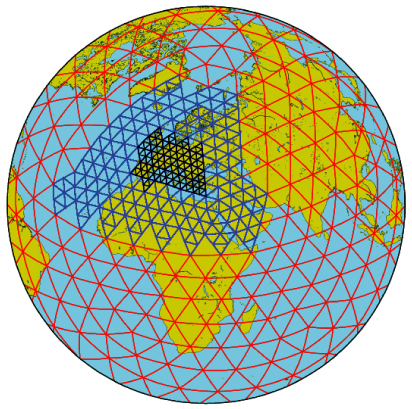
\includegraphics[height=200px]{bilder/gitternetz}
    \caption{Dreiecksgitter des \textit{ICON} Wettermodells (Quelle:
      Deutscher Wetterdienst)}
    \label{gitternetz}
  \end{center}
\end{figure}

Mit der Maschenweite bezeichnet man den horizontalen Abstand zwischen
zwei benachbarten Gitterpunkten. Je feiner das Gitter bzw. je höher
die Auflösung des Modells ist, desto genauer können die Erdoberfläche
und die darüber liegenden atmosphärischen Strukturen erfasst werden,
was sich wiederum auf die Genauigkeit der Wettervorhersage
auswirkt. Die benötigten Ressourcen zur Berechnung der
Modellgleichungen steigt mit der Anzahl der verwendeten Gitterpunkte.

Da eine sehr hohe Auflösung selbst die Leistungsfähigkeit der
schnellsten Supercomputer übersteigt, werden von den Wetterdiensten
meist verschiedene Modelle in unterschiedlichen Auflösungen
berechnet. Globale Modelle, die den gesamten Globus umfassen, werden
mit einer geringeren Auflösung berechnet als lokale Modelle, die nur
einzelne Länder oder Kontinente abdecken. Je weiter aber in die
Zukunft prognostiziert wird, desto mehr spielen aber wieder
Wetterphänomene aus Gebieten, die nicht vom lokalen Modell abgedeckt
werden eine Rolle. Für Vorhersagen ab 5 Tagen in die Zukunft benötigen
die lokalen Modelle wiederum Informationen aus der gesamten
Atmosphäre. Deshalb verwenden die höher auflösenden lokalen Modelle
oft Informationen als Randwerte aus einem zuvor berechneten globalen
Modell.

Die zeitliche Diskretisierung hingegen ist weniger problematisch. Die
meisten Modelle bieten mindestens Prognosen um 12.00 und 24.00 Uhr für
diejenigen Tage an, über die sich der Vorhersagezeitraum
erstreckt. Das \textit{Global Forecast System} und das \textit{Wave
  Watch III} Modell bieten Vorhersagen im drei Stunden-Intervall an,
das lokale \textit{COSMO-DE} Modell sogar in einem Intervall von 25
Sekunden.

\subsubsection{Rechenaufwand heutiger Modelle}

In einer Präsentation
\footnote{\url{http://www.initiative-wissenschaftsjournalismus.de/fileadmin/Downloads/WissensWerte2008/B3_Majewski.pdf}}
aus dem November 2008 wurde der Rechenaufwand für die vom Deutschen
Wetterdienst betriebenen Modelle mit den dazugehörigen Kenngrößen
veröffentlicht. Damals wurden die Wettervorhersagen auf einem IBM
Power 5 System (p575) mit 52 Knoten, 416 Prozessoren und einer
Spitzenleistung von 3,1 Teraflop/s berechnet.

\begin{itemize}
\item Für Deutschland wird das \textit{COSMO-DE} Modell mit einer
  Maschenweite von 2,8 Kilometern betrieben und besteht aus ca. 10
  Millionen Gitterpunkten. Die Berechnung dauert 30 Minuten und
  liefert Vorhersagen in einem 25 Sekunden Intervall für einen
  21-stündigen Vorhersagezeitraum.
\item Das Europa umfassende Modell \textit{COSMO-EU} hat eine
  Maschenweite von 7 Kilometern, ca. 17 Millionen Gitterpunkten und
  wird mit einem Zeitintervall von 40 Sekunden erstellt. Die
  Berechnung einer 24-stündigen Vorhersage dauert 25 Minuten.
\item Das globale, die gesamte Welt umfassende \textit{GME} Modell hat
  eine Maschenweite von 40 Kilometern mit ca. 15 Millionen
  Gitterpunkten. Die Berechnung der 24-stündigen Vorhersage mit einem
  Zeitintervall von 133 Sekunden benötigt 15 Minuten.
\end{itemize}

Leider wurden während der Recherche keine genaueren Informationen
gefunden, wie sich die Berechnung der hier erwähnten Modelle auf dem
seit März 2009 beim Deutschen Wetterdienst in Betrieb genommenen
Vektorsupercomputer SX-9 der Firma NEC verhält. Die Spitzenleistung
dieses Systems beträgt momentan 4,5 Teraflop/s, die bis 2010 auf 11
Teraflop/s aufgestockt werden soll. Mit dieser neuen Anschaffung will
der Deutsche Wetterdienst unter anderem auch Wettervorhersagen mit
einer Auflösung von 2,8 Kilometern für Deutschlands Anrainerstaaten
berechnen.

\subsection{Geographische Breite und Länge}
Zur Festlegung von Punkten auf der Erde wird meist ein
Koordinatensystem genutzt, dessen Grundlage parallel zum Äquator
verlaufende Breitenkreise und die beiden Pole verbindende
Längenhalbkreise sind. Der am Äquator angesiedelte Breitenkreis teilt
die Erde in die nördliche und die südliche Halbkugel. Sowohl auf dem
nördlichen als auch auf dem südlichen Teil verlaufen jeweils weitere
90 Kreise, den Äquator mit eingeschlossen, also insgesamt 181
Breitenkreise. Die beiden Pole werden durch 360 nebeneinander liegende
Längenhalbkreise verbunden, von denen der durch die Sternwarte in
\textit{Greenwich} verlaufende Halbkreis als Nullmeridian bezeichnet
wird. Die Zählung fängt am Nullmeridian an, und geht jeweils um 180
Schritte in beide Richtungen. Nullpunkt des Koordinatensystems ist
derjenige Punkt, an dem der Nullmeridian den Äquator kreuzt. In
Abbildung \ref{koordinaten} ist der durch \textit{Greenwich} laufende
Nullmeridian und der 30 $^\circ$ nördlich verlaufende Breitenkreis zu
sehen.

\begin{figure}[h]
  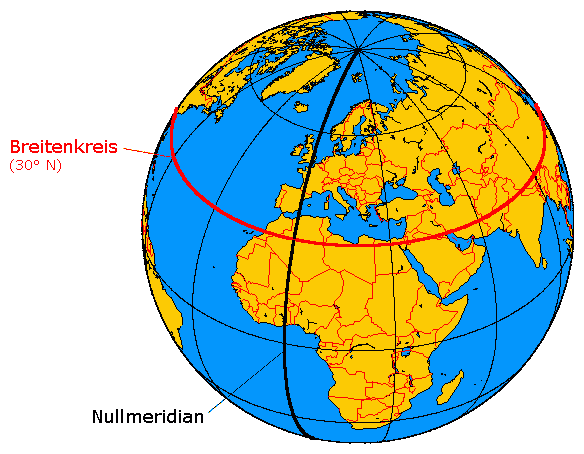
\includegraphics[width=310px]{bilder/koordinaten}
  \caption{Die in Breiten- und Längenkreise unterteilte Erdkugel (Quelle: Wikipedia)}
  \label{koordinaten}
\end{figure}

Die Position eines Punktes auf der Erde wird durch seine geographische
Breite (\textit{Latitude}) und Länge (\textit{Longitude})
angegeben. Dies sind die in der Einheit Grad angegebenen, und vom
Nullpunkt aus gesehenen Abstände der durch diesen Punkt verlaufenden
Breiten- und Längenkreise. Die Position von \textit{Greenwich} ist
beispielsweise durch die Angabe \textit{51.479 $^\circ$ N, 0.0
  $^\circ$ E} festgelegt.


\subsection{Angaben zur Modellauflösung}
Das \textit{Global Forecast System} und das \textit{Wave Watch III}
Modell beziehen sich ebenfalls auf dieses Koordinatensystem, und deren
Gitterauflösung wird in der Einheit Grad angegeben. Da die meisten
Menschen aber bei Distanzangaben in einer Längeneinheit denken an die
sie gewöhnt sind und unter der sie sich auch etwas vorstellen können,
stellt sich die Frage, wie viele Kilometer bzw. Meilen der Abstand
zwischen zwei Knotenpunkten des Gitternetzes beträgt.

Aufgrund der elipsoiden Gestalt der Erdkugel kann hierzu jedoch keine
allgemeingültige Aussage getroffen werden, da dies von der jeweils
betrachteten Region auf der Erdkugel und dem verwendeten
Referenzellipsoiden abhängig ist. Ein Breitengrad (\textit{Latitude})
entspricht durchschnittlich etwa 111 Kilometern und ist weitestgehend
konstant. Der Abstand zwischen den Längengraden (\textit{Longitude})
variiert allerdings erheblich. Am Äquator beträgt dieser Abstand
ebenfalls ungefähr 111 Kilometer, konvergiert aber an den Polen in
Richtung Null. Die hier teilweise in Kilometern angegebenen
Gitterauflösungen sind demnach nur als grobe Richtwerte zur besseren
Einschätzung der Gitterauflösung zu verstehen und beziehen sich auf
die Regionen um den Äquator. Eine praktische Zusammenfassungen mit
Formeln zur Berechnung von Problemen aus dem geographischen Bereich
sind unter \cite{aviation} und \cite{movable_type_scripts} zu finden.

\subsection{Global Forecast System}
Das \textit{Global Forecast System} ist ein globales numerisches
Wettermodell, das vom \textit{National Weather Service} betrieben wird
und den gesamten Erdball abdeckt. Da die Ergebnisse der
Modellberechnung über das Internet
\footnote{\url{http://nomad5.ncep.noaa.gov/pub/gfs}} erhältlich sind
und von jedem verwendet werden dürfen, erfreut es sich einer großen
Beliebtheit. Das Modell liefert Vorhersagen bis zu 384 Stunden (16
Tage) in die Zukunft und wird mit variierenden Auflösungen viermal
täglich berechnet, jeweils um 6.00, 12.00 und 18.00 und 24.00 Uhr
koordinierter Weltzeit (\textit{UTC}). Die ersten 180 Stunden werden
mit einer Maschenweite von ca. 40 Kilometern und einem Intervall von 3
Stunden berechnet, die restlichen Stunden im 12-Stunden-Intervall und
einer Auflösung von ca. 80 Kilometern. Vertikal wird die Atmosphäre
bei beiden Auflösungen in 64 unterschiedliche Luftschichten
aufgeteilt.

Das Modell berechnet eine Vielzahl von physikalischen Größen, von
denen hier hauptsächlich die Temperatur, die Gesamtbewölkung und das
Niederschlagswasser von Bedeutung sind. Da weithin Einverständnis
darüber herrscht, dass Vorhersagen über 180 Stunden hinaus sehr
ungenau sind, verwenden die hier entwickelten \textit{ETL} Prozesse
nur die ersten 180 Stunden in der höchsten Auflösung.

\subsection{Wave Watch III}
Um für mehr Sicherheit auf hoher See und an Küstenregionen zu sorgen,
betreibt der \textit{National Weather Service} das \textit{Wave Watch
  III} Wettermodell, um Wellen vorherzusagen. Es liefert
ausschließlich Informationen über diejenigen Wellen, die durch den
direkten Einfluss von Winden entstehen. Wellen, die durch andere
Ereignisse wie z.B. Gewitter, Gezeiten oder Tsunamis verursacht
werden, sind in diesem Modell nicht berücksichtigt. Da sich Wellen
viel zu sehr voneinander unterscheiden, werden nicht Vorhersagen für
einzelne Wellen getroffen, sondern über die Statistik von mehreren
Wellen. Das Modell liefert sowohl Informationen über die Wellenhöhe,
die Wellenperiode und die Wellenrichtung als auch über die Windstärke
und die Windrichtung.

Das Modell wird wie das \textit{Global Forecast System} viermal
täglich neu berechnet und liefert Vorhersagen im 3-Stunden-Intervall
für 180 Stunden in die Zukunft. Die Ergebnisse sind ebenfalls frei
erhältlich
\footnote{\url{http://polar.ncep.noaa.gov/waves/index2.shtml}}. Das
globale Modell wird mit einer Maschenweite von ca. 80 Kilometern
berechnet, die lokalen Modelle mit einer Maschenweite von bis zu 20
Kilometern. Die hier entwickelten \textit{ETL} Prozesse verarbeiten
bisher nur die Daten des globalen Modells. Die Integration der lokalen
Modelle ist für eine der nächsten Versionen der Web-Applikation
geplant, um insbesondere in den Küstenregionen bessere Ergebnisse
anbieten zu können.

\section{Das Gridded Binary Datenformat}
Die Abkürzung \textit{Grib} \nomenclature{GRIB}{Gridded Binary} steht
für \textit{GRIdded Binary} und ist ein bitorientiertes Datenformat
zum Speichern und Übertragen von Wetterdaten. Das Format wurde von der
\textit{Kommission für Basissysteme} (\textit{CBS})
\nomenclature{CBS}{Commission for Basic Systems} der
\textit{Weltorganisation für Meteorologie} (\textit{WMO})
\nomenclature{WMO}{World Meteorological Organization} standardisiert
\footnote{\url{http://www.wmo.int/pages/prog/www/WMOCodes/Guides/GRIB/GRIB1-Contents.html}}
und wird von vielen Wetterorganisationen dazu verwendet die Ergebnisse
ihrer Modellberechnungen kompakt und plattformunabhängig zu speichern
und auszutauschen. Insgesamt wurden drei verschiedene Versionen
spezifiziert, von denen sich mittlerweile die Versionen 1 und 2
etabliert haben. Die mit der Nummer 0 bezeichnete Version gilt als
veraltet und befindet sich bei den meisten Wetterorganisationen nicht
mehr im operativen Einsatz.

\subsection{Struktur von Grib-Dateien}
Eine \textit{Grib}-Datei besteht aus eigenständigen, sich selbst
beschreibenden Datensätzen, den sogenannten \textit{Grib}
Nachrichten. Eine Nachricht enthält dabei alle Daten eines bestimmten
Vorhersageelements, für eine auf ein Gitternetz diskretisierte
geographische Region zu einem bestimmten Zeitpunkt. Beispielsweise die
Temperaturen um 12.00 Uhr mittags der gesamten Erdkugel aus dem
\textit{Global Forecast System} oder die signifikanten Wellenhöhen des
\textit{Wave Watch III} Modells um 9.00 Uhr morgens für Europa.

Eine \textit{Grib}-Nachricht besteht wiederum aus mehreren Sektionen,
die den Inhalt einer Nachricht genauer beschreiben und in Tabelle
\ref{tab:grib} aufgelistet sind. Die Sektionen enthalten neben den
eigentlichen Daten Informationen über die Dimension und Auflösung des
verwendeten Gitternetzes, die Herkunft der Daten, die Art des
verwendeten Komprimierungsverfahrens und die physikalische Einheit, in
der die Daten gespeichert sind. \textit{Grib}-Nachrichten können
beliebig oft aneinander gereiht werden, was eine individuelle
Komposition von unterschiedlichen Nachrichten in einer Datei
erlaubt. Dies wird in Abschnitt \ref{subsec:download} ausgenutzt, um
nur ausgewählte Nachrichten aus einer größeren \textit{Grib}-Datei zu
beziehen.

\begin{table*}
  \centering
  {\sf
    \footnotesize
    \begin{longtable}{@{}lp{10cm}@{}}

      \toprule
      \textbf{Name der Sektion} & \textbf{Verwendungszweck} \\

      \midrule

      Indicator & Die Zeichenkette ''GRIB'', Versionsnummer, Länge der gesamten Nachricht \\

      Identification & Charakteristiken, die auf alle Daten zutreffen, u.a. Herkunft der Daten, Referenzzeit und Typ des Produkts \\

      Local Use (optional) & Abschnitt für beliebige zusätzliche Informationen \\

      Grid Definition &  Definition des Gitternetzes, u.a. die Dimension, die Anzahl der Datenpunkte und die verwendete Koordinatenprojektion \\

      Product Definition &  Beschreibung der Daten, Temperatur, Wellenhöhe, etc. \\

      Data Representation &  Beschreibung, wie die Daten repräsentiert werden. Art der Komprimierung \\

      Bitmap & Eine Bitmap, welche die Anwesenheit bzw. Abwesenheit von Datenpunkten in der nächsten Sektion signalisiert \\

      Data &  Die komprimierten Daten. Für jeden in der Bitmap existierenden Gitterpunkt ein Wert. \\

      End & Die Zeichenkette ''7777'' markiert das Ende der Nachricht \\

      \bottomrule

    \end{longtable}
  }

  \caption{Die Sektionen einer \textit{Grib}-Nachricht (Version 2)}
  \label{tab:grib}

\end{table*}

\subsection{Programme zum Verarbeiten von Grib-Dateien}
\label{grib-reader}
Zum Verarbeiten und Lesen von \textit{Grib}-Dateien werden spezielle
Programme eingesetzt. Werkzeuge für die Kommandozeile, C-Bibliotheken
und Programme zur Visualisierung der \textit{Grib}-Daten sind für
verschiedene Plattformen und Programmiersprachen erhältlich. Eine
Übersicht gängiger Software ist bei \textit{Wikipedia}
\footnote{\url{http://en.wikipedia.org/wiki/GRIB\#Applications}} zu
finden. Zur Weiterverarbeitung sind insbesondere die
Kommandozeilenprogramme \texttt{wgrib} und \texttt{degrib} zu
empfehlen, da sie als typische \textit{UNIX}-Filter konzipiert sind
und in Kombination mit Standardwerkzeugen wie \texttt{cat},
\texttt{curl} oder \texttt{dd} flexibel eingesetzt werden können. Das
Programm \texttt{degrib} bietet zudem die Möglichkeit, einen Index für
eine \textit{Grib}-Datei zu erstellen, mit dessen Hilfe ein wahlfreier
Zugriff nach geographischen Positionen ermöglicht wird und die
Zugriffszeiten erheblich beschleunigt.

\subsection{Inventar einer Grib-Datei}
Die beiden Kommandozeilenprogramme \texttt{degrib} und \texttt{wgrib}
können dazu verwendet werden, Inventare von \textit{Grib}-Datei zu
erstellen. Ein Inventar ist eine Art Inhaltsverzeichnis und liefert
Informationen über die in der Datei enthaltenen Nachrichten. Da
\textit{Grib}-Dateien oft mehrere Megabyte groß sind, stellen viele
Wetterorganisationen aus praktischen Gründen zusätzlich die Inventare
zur Verfügung. Ein Inventar ist zur Verarbeitung einer \textit{Grib}
Datei zwar nicht zwingend erforderlich, vereinfacht aber den Umgang,
da zur Inspektion nicht immer die kompletten \textit{Grib}-Dateien
übertragen werden müssen, sondern nur die sehr viel kleineren
Inventare. In Abbildung \ref{abbildung:inventar} ist der Ausschnitt
eines Inventars von einer \textit{Grib}-Datei des \textit{Global
  Forecast System} zu sehen. Pro Nachricht ist in diesem Inventar eine
Zeile enthalten, die unter anderem Informationen über die Nummer der
Nachricht, deren Position in Bytes und den Zeitpunkt als auch das
Element der Vorhersage liefert.

\begin{figure}[h]
  \begin{Verbatim}[frame=lines,framerule=0.5pt,framesep=3mm]
    1:0:d=2009081812:HGT:10 mb:anl:NAve=0
    2:519924:d=2009081812:TMP:10 mb:anl:NAve=0
    3:812418:d=2009081812:UGRD:10 mb:anl:NAve=0
    ...
    568:211123530:d=2009081812:VWSH:-1500 pv units:anl:NAve=0
  \end{Verbatim}
  \caption{Inventar einer \textit{Grib}-Datei des \textit{Global
      Forecast System} }
  \label{abbildung:inventar}
\end{figure}

Die zweite Zeile aus Abbildung \ref{abbildung:inventar} gibt zum
Beispiel Auskunft darüber, dass die Nachricht mit der Nummer 2 in der
\textit{Grib}-Datei an der Position 519.924 (Byte) zu finden ist, die
Werte der Nachricht für den 18. August 2009 um 12.00 Uhr gelten und
das Element die Temperatur (TMP) auf einer Höhe von 10 Hektopascal (10
mb) darstellt. Zudem handelt es sich bei den Werten nicht um eine
Vorhersage (fcst), sondern um eine Analyse (anl) für die hier kein
durchschnittlicher Wert (NAve=0) berechnet ist. Mit Analyse wird hier
der Ausgangszustand der Atmosphäre zum Zeitpunkt der Modellberechnung
bezeichnet und mit Vorhersage der simulierte Zustand in der
Zukunft. Diese Inhaltsverzeichnisse werden in den
\textit{ETL}-Prozessen verwendet, um nur die benötigten Nachrichten
einer \textit{Grib}-Datei zu extrahieren.

\section{Extraktion aus dem Quellsystem}
Die Aufgabe der hier entwickelten Extraktionsprozesse besteht darin,
die benötigten Daten des \textit{Wave Watch III} Models und des
\textit{Global Forecast Systems} herunterzuladen und diese in einer
einheitlichen Struktur für die Weiterverarbeitung im lokalen
Dateisystem zu hinterlegen. Da insbesondere das Datenvolumen des
\textit{Global Forecast System} in seiner höchsten Auflösung sehr
umfangreich ist (ca. 13 GB), wird ein Verfahren angewendet, um nur
ausgewählte Daten zu beziehen. In diesem Abschnitt wird zuerst die
Struktur des Quellsystems analysiert, dann das Verfahren zum Download
der ausgewählten Daten vorgestellt und anschließend eine Aussage über
die Performanz des Extraktionsprozesses getroffen.

\subsection{Analyse der Quellsystems}
Sowohl das \textit{Global Forecast System} als auch das \textit{Wave
  Watch III} Modell werden viermal täglich, jeweils um , 6.00, 12.00,
18.00 und 24.00 Uhr koordinierter Weltzeit (UTC) berechnet. Danach
werden die Ergebnisse in \textit{Grib}-Dateien auf mehreren, teilweise
von Unterorganisationen der \textit{NOAA} betriebenen Servern
veröffentlicht, die verschiedensten Anforderungen gerecht werden. Auf
einigen Servern sind nur die aktuellen Ergebnisse verfügbar, andere
wiederum dienen der Archivierung und bieten eine Historie über mehrere
Jahre hinweg.

Die Ergebnisse der Modellberechnung werden in einem, meist nach Datum
und Uhrzeit strukturiertem Dateisystem hinterlegt, das per
\textit{FTP} oder \textit{HTTP} exportiert wird. Die Struktur und
Benennung der Verzeichnisse und Dateien variiert dabei zwischen den
Servern, ist aber innerhalb eines Servers konsistent und folgt einem
vorhersehbaren Muster. Die \textit{URI}s der benötigten Daten können
so für einen bestimmten Server im voraus konstruiert werden und die
Existenz der \textit{Grib}-Daten mit einem der unterstützten
Protokolle überprüft werden. Dieses Verfahren ist ein Beispiel zur
Identifizierung von Ressourcen durch vorhersehbare \textit{URI}s und
ist einer der in Abschnitt \ref{paragraph:identifizierung}
beschriebenen Vorschläge aus der \textit{Ressource Oriented
  Architecture}.

\subsubsection{Datenorganisation des Global Forecast System}
Aktuelle Daten des \textit{Global Forecast System} können in
verschiedenen Auflösungen von den Servern des \textit{National Oceanic
  and Atmospheric Administration Operational Model Archive and
  Distribution System (NOMADS)} \nomenclature{NOMADS}{NOAA Operational
  Model Archive and Distribution System}
\footnote{\url{http://nomads.ncdc.noaa.gov}} bezogen werden. In
Tabelle \ref{tab:gfs_auflösungen} sind die Dateigrößen und
Bezugsquellen der \textit{Grib}-Dateien in den verschiedenen
Auflösungen dargestellt. Die Dateigröße bezieht sich dabei immer auf
eine einzelne \textit{Grib}-Datei, die alle Vorhersageelemente des
\textit{Global Forecast System} für einen bestimmten Zeitpunkt in der
Zukunft enthält.

\begin{table*}[h]
  \centering
  {\sf
    \footnotesize
    \begin{longtable}{@{}ccl}
      \toprule
      \textbf{Auflösung} & \textbf{Dateigrößen} & \textbf{URI der Bezugsquelle} \\
      \midrule
      2$^{\circ}$ x 5$^{\circ}$ & 4 MB - 4.8 MB & \url{http://nomad5.ncep.noaa.gov/pub/gfs2p5} \\
      1$^{\circ}$ x 1$^{\circ}$ & 25 MB - 29 MB & \url{http://nomad5.ncep.noaa.gov/pub/gfs} \\
      0.5$^{\circ}$ x 0.5$^{\circ}$ & 200 MB - 215 MB & \url{http://nomad5.ncep.noaa.gov/pub/gfs_master} \\
      \bottomrule
    \end{longtable}
  }
  \caption{Dateigrößen des \textit{Global Forecast System}}
  \label{tab:gfs_auflösungen}
\end{table*}

Die in dieser Arbeit entwickelten \textit{ETL}-Prozesse arbeiten alle
mit den \textit{Grib}-Dateien der höchsten Auflösung (0.5$^{\circ}$ x
0.5$^{\circ}$). Unter der \textit{URI}
\url{http://nomad5.ncep.noaa.gov/pub/gfs_master/} sind Verzeichnisse
zu finden, die nach dem Muster \texttt{gfs\textbf{\textit{YYYYMMDD}}} benannt
sind. Dabei steht \texttt{YYYY} für das Jahr, \texttt{MM} für den
Monat und \texttt{DD} für den Tag, an dem ein Modell berechnet
wurde. Beispielsweise waren die \textit{Grib}-Dateien aller
Modellberechnungen, die am 16. August 2009 durchgeführt wurden, unter
der \textit{URI}
\url{http://nomad5.ncep.noaa.gov/pub/gfs_master/gfs20090816/}
aufgelistet.  \footnote{Der Server \texttt{nomad5.ncep.noaa.gov}
  verwaltet keine historischen Daten, d.h. wenn dieses Dokument
  gelesen wird, sind höchstwahrscheinlich keine Daten mehr für die
  hier verwendeten Tage vorhanden.}

In den nach Tagen geordneten Verzeichnissen befinden sich
\textit{Grib}-Dateien, die nach dem Muster
\texttt{gfs.t\textbf{XX}z.master.grbf\textbf{YY}} benannt sind. Die
Zeichen \texttt{XX} stehen dabei für den Zeitpunkt der
Modellberechnung (00, 06, 12 oder 18), und die Zeichen \texttt{YY} für
die Stunde der Vorhersage in der Zukunft (00-180 im 3 Stunden
Intervall). Die Vorhersagedaten des \textit{GFS} für den 16. August
2009 um 18 Uhr abends, die am selben Tag um 6 Uhr morgens berechnet
wurden, waren somit in der \textit{Grib}-Datei mit dem \textit{URI}
\url{http://nomad5.ncep.noaa.gov/pub/gfs_master/gfs20090816/gfs.t06z.master.grbf12}
zu finden.

Eine \textit{Grib}-Datei des \textit{Global Forecast System} enthält
für einen bestimmten Zeitpunkt 63 verschiedene Vorhersageelemente und
ist zwischen 200 und 215 Megabyte groß. Die Größe aller \textit{Grib}
Daten für einen Vorhersagezeitraum von 180 Stunden (und für den
Berechnungszeitpunkt selbst) mit einem 3-stündigen Intervall beträgt
somit $(180h / 3h + 1) * 215 MB = 13.115 MB$. Da hier aber nur sehr
wenige Vorhersageelemente der \textit{Grib}-Dateien benötigt werden,
wird in Abschnitt \ref{subsec:download} ein Verfahren vorgestellt, um
nur die benötigten Elemente zu übertragen und somit das zu
übertragende Datenvolumen zu reduzieren.

\subsubsection{Datenorganisation des Wave Watch III Models}
Die Daten des \textit{Wave Watch III} Modells sind ähnlich
strukturiert wie die des \textit{Global Forecast System} und werden in
einer Auflösung von 1.25$^{\circ}$ x 1$^{\circ}$ ebenfalls auf den
\textit{NOMADS} Servern veröffentlicht. Die \textit{Grib}-Dateien
werden in Verzeichnissen hinterlegt, die nach dem Muster
\texttt{nww3\textbf{YYYYMMDD}} benannt und unter der \textit{URI}
\url{http://nomad5.ncep.noaa.gov/pub/waves/nww3} angeordnet sind. Auch
hier ist das Datum der Modellberechnung im Verzeichnisnamen
kodiert. Das \textit{Wave Watch III} Modell hat im Vergleich zum
\textit{Global Forecast System} viel weniger Elemente, weshalb die
kompletten Daten für eine 180-stündige Vorhersage in einer einzigen
Datei gespeichert werden. Diese ist nach dem Muster
\texttt{nww3.t\textbf{XX}z.grib} benannt, wobei \texttt{XX} hier
ebenfalls für den Zeitpunkt der Modellberechnung (00, 06, 12 oder 18)
steht. Die Ergebnisse des \textit{Wave Watch III} Modells, das z.B. am
16. August 2009 um 18 Uhr berechnet wurde, konnten unter dem
\textit{URI}
\url{http://nomad5.ncep.noaa.gov/pub/waves/nww3/nww320090816/nww3.t18z.grib}
bezogen werden.

Eine \textit{Grib}-Datei des \textit{Wave Watch III} Models mit 11
verschiedenen Elementen ist bei einer Auflösung von
1.25$^{\circ}$ x 1$^{\circ}$ ca. 32 Megabyte groß und enthält
Vorhersagedaten für 180 Stunden in die Zukunft.

\subsection{Download einzelner Grib-Nachrichten}
\label{subsec:download}
Die beiden Vorhersagemodelle bieten sehr viel mehr Informationen, als
von der hier entwickelten Anwendung überhaupt benötigt werden. Vom
\textit{Global Forecast System} werden im Moment lediglich 4 der 63
verschiedenen Vorhersagelemente und vom \textit{Wave Watch III} Modell
7 von 11 Elementen verwendet. Um nicht unnötig Bandbreite zu
verschwenden und den Extraktionsprozess zu beschleunigen, wird hier
ein Verfahren angewendet, das in dem Dokument \textit{Fast Downloading
  of Grib Files}
\footnote{\url{http://www.cpc.noaa.gov/products/wesley/fast_downloading_grib.html}}
beschrieben ist. Ziel ist es, nur die gewünschten Nachrichten einer
\textit{Grib}-Datei herunterzuladen. Voraussetzung dafür ist, dass die
Dateien von einem Server bezogen werden, der das HTTP/1.1 Protokoll
unterstützt und die Inhaltsverzeichnisse der Dateien zu Verfügung
stehen. Das Verfahren besteht aus den folgende drei Schritten.

\begin{enumerate}
\item Download des Inhaltsverzeichnisses der entsprechenden Datei
\item Berechnung der Start- und Endpositionen aller relevanten Nachrichten
\item Download der entsprechenden Nachricht (\textit{HTTP Range Header})
\end{enumerate}

Im ersten Schritt wird das Inhaltsverzeichnis der entsprechenden
\textit{Grib}-Datei heruntergeladen. Die Inhaltsverzeichnisse auf den
\textit{NOMADS} Servern sind mit dem Programm \textit{wgrib} erstellt
und deren \textit{URI} lässt sich durch das Anhängen der Endung
''.inv'' an die \textit{URI} der \textit{Grib}-Datei konstruieren.

Anschließend wird im zweiten Schritt in Zweierpaaren über die Zeilen
des Inhaltsverzeichnisses iteriert. Dabei wird die Startposition jeder
Nachricht extrahiert und die dazugehörige Endposition berechnet. Die
Startposition steht dabei an zweiter Stelle jeder Zeile und die
Endposition berechnet sich aus der Startposition der nächsten
Nachricht, von der ein Byte subtrahiert wird. Ein Sonderfall ist die
letzte Nachricht des Inhaltsverzeichnisses. Für diese Nachricht kann
die Endposition nicht berechnet werden, da keine Information über die
gesamte Länge der \textit{Grib} im Inhaltsverzeichnis vorhanden
ist. Tabelle \ref{tab:inhaltsverzeichnis_mit_positionen} zeigt das
Resultat dieser Berechnung, angewendet auf das Inhaltsverzeichnis aus
Abbildung \ref{abbildung:inventar}.

\begin{table*}[h]
  \centering
  {\sf
    \footnotesize
    \begin{longtable}{@{}ccccc}
      \toprule
      \textbf{Nachricht} & \textbf{Startposition} & \textbf{Endposition} & \textbf{Referenzzeit} & \textbf{Element} \\
      \midrule
      1 & 0 & 519.923 & 2009-08-18 12:00 & HGT \\
      2 & 519.924 & 812.417 & 2009-08-18 12:00 & TMP \\
      3 & 812.418 & ... & 2009-08-18 12:00 & UGRD \\
      ... & ... & ... & ... & ... \\
      568 & 211.123.530 & - & 2009-08-18 12:00 & HGT \\
      \bottomrule
    \end{longtable}
  }

  \caption{Berechnete Positionen aus einem Inhaltsverzeichnis}
  \label{tab:inhaltsverzeichnis_mit_positionen}

\end{table*}

Im dritten Schritt werden schließlich nur die ausgewählten Nachrichten
unter Verwendung des \textit{HTTP/1.1} Protokolls
heruntergeladen. Dabei wird pro Nachricht eine Anfrage an den Server
gesendet, in der die Start- und Endposition im \textit{Range} Feld des
\textit{HTTP} Headers eingetragen wird. Um beispielsweise nur die
zweite Nachricht aus Tabelle
\ref{tab:inhaltsverzeichnis_mit_positionen} herunterzuladen, wird das
\textit{Range} Feld auf ''bytes=519924-812417'' gesetzt. Der im
zweiten Schritt erwähnte Sonderfall, bei dem die Endposition für die
letzte Nachricht nicht bekannt ist, wird dadurch abgedeckt, dass die
Endposition im \textit{Range} Header einfach weggelassen wird. Dies
ist trotz der fehlenden Endposition eine gültige \textit{Range} Angabe
und veranlasst den Server dazu, den Rest der Datei ab der gegebenen
Startposition zu senden. Zum Download der einzelnen
\textit{Grib-}Nachrichten wird das Programm \textit{curl}
\footnote{\url{http://curl.haxx.se}} verwendet, da es das
\textit{HTTP/1.1} Protokoll unterstützt und man beliebige Felder im
\textit{HTTP} Header angeben kann.

\subsection{Beschreibung der Extraktionsprozesse}
Ziel der Extraktion ist es, alle relevanten \textit{Grib}-Nachrichten
der beiden Modelle in einer einheitlichen Struktur im lokalen
Dateisystem zu hinterlegen. Pro Element wird eine Datei erstellt
werden, die alle Nachrichten des entsprechenden Elements für die
verschiedenen Zeitpunkte der Vorhersage enthält. Beim Download der
\textit{Grib}-Dateien von den \textit{NOMADS} Servern werden zwei
verschiedene Strategien angewendet, die im Folgenden beschrieben
werden. Dies ist auf die unterschiedliche Datenorganisation der beiden
Vorhersagemodelle auf der Serverseite zurückzuführen.

Die Performanz der Extraktionsprozesse hängt hauptsächlich von der
Geschwindigkeit ab, mit der die \textit{Grib}-Daten heruntergeladen
werden. Um die durchschnittliche Übertragungsgeschwindigkeit über
einen längeren Zeitraum zu ermitteln, wurden mehrere Messung durch
einen \textit{Cronjob} mit dem Kommandozeilenprogramm \textit{ab}
\footnote{Apache HTTP Server Benchmarking Tool} durchgeführt, wobei
jedes mal eine 32 MB große \textit{Grib}-Datei heruntergeladen
wurde. Die Messwerte wurden in einem Intervall von 6 Stunden über
einen Zeitraum von einer Woche erhoben. Dieser Messintervall
entspricht dem Intervall, in dem die beiden Modelle aktualisiert
werden. Alle 28 Messungen sind auf einem dedizierten Server ausgeführt
worden, der mit einer 100 Mbps Verbindung an das Internet
angeschlossen ist. Das Ergebnis der Messung ergab eine eher mäßige
durchschnittliche Übertragungsgeschwindigkeit von 166,22 KB/s mit
einer Standardabweichung von 40,5 KB/s. Die schlechte
Übertragungsgeschwindigkeit liegt vermutlich an der hohen Auslastung
der \textit{NOMADS} Server, auf die keinen Einfluss genommen werden
kann. Um eine Aussage über die Laufzeit der Extraktionsprozesse zu
machen, wurden die Log Dateien der beiden Prozesse ebenfalls über
einen Zeitraum von einer Woche ausgewertet und die Ergebnisse
zusammengefasst. Die durchschnittlichen Laufzeiten wurden für jedes
Modell aus insgesamt 28 Messwerten berechnet.

\begin{table*}[h]
  \centering
  {\sf
    \footnotesize
    \begin{longtable}{@{}clccc}
      \toprule
      \textbf{Element} & \textbf{Beschreibung} & \textbf{Größe (Element)} & \textbf{Zeit (Element)}  \\
      \midrule
      HTSGW & Wellenhöhe & 2,5 MB &  27 s \\
      PERPW & Periode des Wellenkamms & 2,7 MB &  30 s \\
      DIRPW & Richtung des Wellenkamms & 3,5 MB &  37 s \\
      WVPER & Wellenperiode & 2,5 MB &  26 s \\
      WVDIR & Wellenrichtung & 3,5 MB &  36 s \\
      WIND  & Windstärke & 2,9 MB &  34 s \\
      WDIR  & Windrichtung & 3,8 MB &  39 s \\
      \midrule
      Gesamt: & & 21,4 MB &  3 min 49 s \\
      \bottomrule
    \end{longtable}
  }
  \caption{Durchschnittliche Downloadzeiten des \textit{Wave Watch III} Modells}
  \label{tab:download_messung_ww3}
\end{table*}

\subsubsection{Downloadstrategie für das Wave Watch III Model}
Alle Daten des \textit{Wave Watch III} Modells sind auf Serverseite in
einer \textit{Grib}-Datei gespeichert. Der Extraktionsprozess für
dieses Modell lädt zunächst das Inhaltsverzeichnis dieser Datei, um
die Start- und Endpositionen der gewünschten Elemente zu
berechnen. Anschließend wird pro Element eine \textit{HTTP-Range}
Anfrage an den Server gesendet und die in der Antwort enthaltene
\textit{Grib}-Nachricht in einer Datei im lokalen Dateisystem
gespeichert. Nachdem die Datei gespeichert wurde, wird für den
späteren Transformationsvorgang noch ein Index mit dem Programm
\textit{degrib} erstellt. Insgesamt werden dabei 8 Anfragen an den
Server gesendet, eine für das Inhaltsverzeichnis und 7 für die
\textit{Grib}-Nachrichten der entsprechenden Elemente. In Tabelle
\ref{tab:download_messung_ww3} sind die durchschnittlichen
Downloadzeiten für die einzelnen Elemente des \textit{Wave Watch III}
Modells aufgeführt. Der Extraktionsprozess dauert durchschnittlich
ca. 4 Minuten und überträgt 21,4 MB an \textit{Grib}-Daten.

\subsubsection{Downloadstrategie für das Global Forecast System}
Der Downloadvorgang für das \textit{Global Forecast System} erfordert
wesentlich mehr Anfragen als der des \textit{Wave Watch III} Modells,
da die Daten auf Serverseite in mehreren Dateien gespeichert sind. Für
jeden Zeitpunkt der Vorhersage existiert auf dem Server eine Datei, in
der die Daten aller Modellelemente für den entsprechenden Zeitpunkt
enthalten sind. Dies sind bei einem Vorhersagezeitraum von 180 Stunden
im 3-stündigen Intervall 61 Dateien, $180h / 3h = 60$ für den
Vorhersagezeitraum und eine weitere für den Zeitpunkt der
Modellberechnung, der sogenannten Analyse.

\begin{table*}[h]
  \centering
  {\sf
    \footnotesize
    \begin{longtable}{@{}clcc}
      \toprule
      \textbf{Element} & \textbf{Beschreibung} & \textbf{Größe (Element)} & \textbf{Zeit (Element)} \\
      \midrule
      TMP   & Temperatur & 18.90 MB &  3 m 47 s \\
      TCDC  & Bewölkung & 13.23 MB &  2 m 56 s \\
      PWAT  & Niederschlag & 18.90 MB &  3 m 56 s \\
      WEASD & Schnee & 17.01 MB &  3 m 34 s \\
      \midrule
      Gesamt: & & 68.04 MB &  14 m 13 s \\
      \bottomrule
    \end{longtable}
  }
  \caption{Durchschnittliche Downloadzeiten des \textit{Global Forecast System}}
  \label{tab:download_messung_gfs}
\end{table*}

Um alle \textit{Grib}-Nachrichten für ein ausgewähltes Element
herunterzuladen, müssen zunächst die 61 Inhaltsverzeichnisse aller
\textit{Grib}-Dateien angefordert werden, damit die Start- und
Endpositionen des Elements berechnet werden können. Anschließend
können die eigentlichen Daten des Elements mit
\textit{Http-Range}-Anfragen aus den 61 \textit{Grib}-Dateien
heruntergeladen werden. Die einzelnen \textit{Grib}-Nachrichten aus
den Dateien werden dann pro Element in einer Datei
zusammengefasst. Dies kann Dank des selbstbeschreibenden Formats der
einzelnen \textit{Grib}-Nachrichten mit Standard-Unix-Kommandos
bewerkstelligt werden, beispielsweise mit \textit{cat TMP.00h.grib
  TMP.03h.grib ... TMP.180h.grib > TMP.0h-180h.grib}. Bis auf das
Anfordern der Inhaltsverzeichnisse muss dieser Vorgang für alle
gewünschten Elemente wiederholt werden. Insgesamt sind $ 61 * (N+1) $
Anfragen nötig, 61 für die Inhaltsverzeichnisse und pro Element
weitere \textit{61} Anfragen für die einzelnen
\textit{Grib}-Nachrichten. Der Extraktionsprozess für das
\textit{Global Forecast System} sendet somit für die zurzeit 4
verwendeten Elemente $ 61 * (4+1) = 305$ Anfragen. Tabelle
\ref{tab:download_messung_gfs} zeigt im linken Teil die Größe einer
einzelnen Nachrichten und die Zeit, die benötigt wird, um diese
herunterzuladen. Im rechten Teil ist die Zusammenfassung dieser Werte
für das jeweilige Element zu sehen. Der Extraktionsprozess für das
\textit{Global Forecast System} überträgt insgesamt 68.04 MB und
benötigt durchschnittlich ca. 14 Minuten.

\subsubsection{Lokales Grib Repository}
Nachdem der Extraktionsvorgang erfolgreich abgeschlossen wurde, liegen
die \textit{Grib}-Daten beider Modelle in einem \textit{Repository}
auf dem lokalen Dateisystem. Das \textit{Repository} ist nach dem
Namen des Modells, dem Zeitpunkt, an dem das Modell erstellt wurde,
und dem Element der Vorhersage organisiert. Diese in Tabelle
\ref{tab:repository} zu sehende Struktur bietet den anschließenden
Transformationsprozessen einen einheitlichen Zugriff auf die Elemente
der beiden Modelle.

\begin{table*}
  \centering
  {\sf
    \footnotesize
    \begin{longtable}{@{}cccl}
      \toprule
      \textbf{Größe} & \textbf{Datum} & \textbf{Uhrzeit} & \textbf{Pfad im Repository} \\
      \midrule
      19 MB & 2009-08-18 & 16:19 & forecasts/gfs/20090818/t06z.PWAT.grib \\
      14 MB & 2009-08-18 & 16:13 & forecasts/gfs/20090818/t06z.TCDC.grib \\
      19 MB & 2009-08-18 & 16:09 & forecasts/gfs/20090818/t06z.TMP.grib \\
      18 MB & 2009-08-18 & 16:24 & forecasts/gfs/20090818/t06z.WEASD.grib \\
      \midrule
      3.5 MB & 2009-08-18 & 15:58 & forecasts/nww3/20090818/t06z.DIRPW.grib \\
      2.4 MB & 2009-08-18 & 15:57 & forecasts/nww3/20090818/t06z.HTSGW.grib \\
      2.8 MB & 2009-08-18 & 15:57 & forecasts/nww3/20090818/t06z.PERPW.grib \\
      3.9 MB & 2009-08-18 & 16:02 & forecasts/nww3/20090818/t06z.WDIR.grib \\
      3.0 MB & 2009-08-18 & 16:01 & forecasts/nww3/20090818/t06z.WIND.grib \\
      3.5 MB & 2009-08-18 & 16:00 & forecasts/nww3/20090818/t06z.WVDIR.grib \\
      2.5 MB & 2009-08-18 & 15:59 & forecasts/nww3/20090818/t06z.WVPER.grib \\
      \bottomrule
    \end{longtable}
  }
  \caption{Verzeichnisstruktur der \textit{Grib}-Daten im lokalen Repository}
  \label{tab:repository}
\end{table*}

\subsubsection{Aktualisierung der Daten durch Polling}
Zwar werden beide Modelle viermal täglich zu festen Zeitpunkten
berechnet, wann genau die \textit{Grib}-Dateien auf den
\textit{NOMADS} Servern zur Verfügung stehen variiert
allerdings. Deshalb wird die Verfügbarkeit neuer Daten mittels
\textit{Polling} überprüft. Die durch \textit{Cronjob} gesteuerten
Prozesse überprüfen in einem bestimmten Intervall die Existenz der
Quelldaten und starten den Extraktionsvorgang erst, wenn neue, noch
nicht integrierte Daten zur Verfügung stehen.

\subsubsection{Beurteilung der Extraktionsprozesse}
Trotz der eher mäßigen Übertragungsgeschwindigkeit kann die Performanz
der beiden Extraktionsprozesse als unproblematisch eingestuft
werden. Kritisch wird es, wenn die von den gesamten
\textit{ETL}-Prozessen beanspruchte Zeit sich dem 4-stündigen
Intervall der Modellberechnung nähert. Die Downloadzeit von 18 Minuten
ist für die zu übertragende Datenmenge zwar sehr schlecht, aber nicht
weiter problematisch. Der Download der \textit{Grib}-Daten beansprucht
im Vergleich zu den anschließenden Transformations- und Ladeprozessen
sehr wenig Ressourcen und wirkt sich nur negativ auf die Aktualität
der Vorhersagen aus. Da gravierende Veränderungen in den Vorhersagen
zwischen zwei Modellberechnungen eher selten sind und die Vorhersagen
nicht in Echtzeit benötigt werden, kann diese Verzögerung
vernachlässigt werden. Da es den Anschein macht, dass die
Übertragungsgeschwindigkeit von den \textit{NOMADS} Servern pro
Verbindung reguliert wird, könnte versucht werden mehrere Anfragen
gleichzeitig zu stellen, um die Daten parallel herunterzuladen und
somit die Performanz zu verbessern. Wohin dies führt ist allerdings
fraglich, da man davon ausgehen kann, dass die Anzahl der Verbindungen
von einer IP-Adresse ebenfalls beschränkt wird, falls schon die
Übertragungsgeschwindigkeit gedrosselt wurde. Um die \textit{NOMADS}
Server nicht unnötig zu überlasten und sich fair gegenüber anderen zu
verhalten wurden Tricks dieser Art nicht weiter verfolgt.

\section{Transformation der Daten}
Nachdem der Extraktionsvorgang erfolgreich abgeschlossen wurde und die
Daten beider Modelle im lokalen \textit{Repository} vorliegen, startet
die Transformationsphase. In dieser Phase wird die bisher noch den
gesamten Globus umfassende Datenmenge auf die in der Datenbank
enthaltenen \textit{Spots} reduziert. Alle relevanten Datensätze
werden dabei in einer \textit{CSV}-Datei
\nomenclature{CSV}{Comma-Separated Values} gespeichert, die im
nächsten Schritt mit dem \textit{Bulk Loader} des
Datenbankmanagementsystems in die Datenbank importiert wird.

\subsection{Auslesen der Vorhersagedaten}
\label{auslesen-der-vorhersagedaten}
Um die Vorhersagedaten aus einer \textit{Grib}-Datei auszulesen, wird
ein sogenannter \textit{Grib Reader} benötigt. Hierfür wird das
Kommandozeilenprogramm \textit{degrib} verwendet, da mit ihm ein
schneller und wahlfreier Zugriff nach geographischen Positionen auf
die Vorhersagedaten einer \textit{Grib}-Datei möglich
ist. Vorhersagewerte für geographische Positionen, die nicht genau auf
einem der Gitterpunkte des Modells liegen, werden von \textit{degrib}
entweder durch \textit{bilineare} oder \textit{nearest-neighbor}
Interpolation berechnet. Durch das Erstellen eines Index kann der
wahlfreie Zugriff auf die Vorhersagedaten einer \textit{Grib}-Datei
beschleunigt werden.

\lstinputlisting[caption={Auslesen der Temperatur in Berlin mit \textit{degrib}},label=degrib]{listings/degrib.txt}

Die Temperatur in Berlin \textit{(52.523, 13.411)} kann mit dem Befehl
in Zeile 1 aus Auflistung \ref{degrib} ermittelt werden. Die hier
verwendete \textit{Grib}-Datei stammt aus der Modellberechnung des
\textit{Global Forecast System} vom 04. September 2009 um 6.00 Uhr und
bietet Vorhersagewerte im 3-stündigen Intervall für 180 Stunden in die
Zukunft. Werden Vorhersagedaten an einer geographischen Position
ausgelesen, an der keine Daten \footnote{Beispielsweise die Wellenhöhe
  in Berlin aus dem \textit{Wave Watch III} Modell} vorhanden sind,
liefert \textit{degrib} Datensätze mit dem als ungültig definierten
Wert \textit{9999.0}.

\subsection{Bestimmung der Wave Watch III Position}
Bevor der eigentliche Transformationsvorgang beschrieben wird, muss
zuvor noch auf eine Eigenart des \textit{Wave Watch III} Modells
eingegangen werden. Bei einigen Spots wird das Auslesen der
Wellenvorhersagen durch die zu grobe Gitterauflösung des Modells und
daraus resultierenden Datenlücken erschwert. Mit einem zusätzlichen
Berechnungsschritt, der für jeden Spot einmalig durchzuführen ist,
kann dieses Problem jedoch für die meisten Spots zufriedenstellend
gelöst werden. In diesem Abschnitt wird zunächst näher auf diese
Datenlücken eingegangen und anschließend ein prototypischer
Algorithmus zur Lösung des Problems vorgestellt.

\subsubsection{Datenlücken im Wave Watch III Modell}
Der Fokus des \textit{Wave Watch III} Modells liegt auf der Vorhersage
von Wellen und den damit verbundenen physikalischen Größen. Im
Ergebnis der Modellberechnung sind deshalb nur Vorhersagedaten für
geographische Positionen enthalten, die sich auch über dem Meer
befinden. Für alle anderen Positionen stehen keine Daten zur
Verfügung. Wegen der groben Gitterauflösung des \textit{Wave Watch
  III} Modells verläuft die Grenze zwischen Land und Meer jedoch nicht
wirklichkeitsgetreu, sondern in einer Zick-Zack-Linie, die sich am
rechteckigen Gitternetz des Modells orientiert. In Abbildung
\ref{positions-bestimmung} ist die Küstenregion um den spanischen Ort
Mundaka mit dem darüber liegenden Gitternetz zu sehen. Die Abbildung
soll verdeutlichen, dass nur an den grün eingefärbten Knotenpunkten
des Gitters Vorhersagedaten existieren. An allen anderen Stellen sind
keine Daten vorhanden, da diese Positionen im Modell als Land
betrachtet werden. Deshalb würde man beim Auslesen der Vorhersagedaten
des \textit{Wave Watch III} Modells an der geographischen Position des
Spots Mundaka nur ungültige Werte erhalten.

\begin{figure}
 
\includegraphics[width=\textwidth]{bilder/locate-position}
 \caption{Visualisierung der Datenlücken im \textit{Wave Watch III}
   Modell}
 \label{positions-bestimmung}
\end{figure}

\subsubsection{Vorhersagedaten aus der näheren Umgebung}
Da sich die meisten Spots aber genau in solchen Küstenregionen
befinden, muss eine zufriedenstellende Alternative gefunden werden, um
für diese Spots trotzdem Vorhersagedaten anbieten zu können. Wie in
der Einleitung erwähnt, werden die an den Spots brechenden Wellen
durch den in weit entfernteren Regionen entstandenen und viele
Kilometer weit gereisten Swell beeinflusst. Zieht man lokale
Gegebenheiten, wie z.B. vorgelagerte Inseln, Hafenbecken oder
abgeschirmte Buchten nicht in Betracht, dann sind die für Surfer
wichtigen Eigenschaften eines großräumig eintreffenden Swells in der
Umgebung eines Spots sehr ähnlich. Deshalb werden in der hier
entwickelten Applikation Vorhersagedaten aus der näheren Umgebung
eines Spots herangezogen, falls an der geographischen Position des
Spots selbst keine Daten vorhanden sind. Das zu lösende Problem
besteht darin, eine alternative Vorhersageposition für diejenigen
Spots zu finden, an deren geographischer Position selbst keine Daten
vorhanden sind.

\subsubsection{Bestimmung der Vorhersageposition durch den Benutzer}
Eine Möglichkeit dieses Problem zu Lösen, wäre den Benutzer beim
Erstellen eines neuen Spots die Vorhersageposition selbst angeben zu
lassen. Auf einer interaktiven Karte könnte man den Spot mit dem
darüber liegenden Gitternetz des \textit{Wave Watch III} Modells
einzeichnen und die gültigen Positionen bzw. Gebiete ähnlich wie in
Abbildung \ref{positions-bestimmung} einfärben. Mit einem Klick auf
die Karte kann der Benutzer dann eine alternative Vorhersageposition
auswählen. Wurde eine Position selektiert, für die keine
Vorhersagedaten vorhanden sind, müsste dies dem Anwender unmittelbar
signalisiert werden. Diese Idee wurde hier aber wegen ihrer
Benutzerunfreundlichkeit nicht weiter verfolgt. Der Nutzer müsste
zunächst über Sinn und Zweck der alternativen Vorhersageposition
aufgeklärt werden. Dies verständlich zu kommunizieren und in einer
intuitiven Benutzeroberfläche darzustellen, wird als eines der
Hauptprobleme bei diesem Ansatz angesehen.  Benutzer der Plattform mit
internen Details der Web-Applikation zu konfrontieren, die zudem nicht
unbedingt sofort verständlich sind, wird als nicht zumutbar
eingestuft. Eine bessere und zudem automatisierte Alternative, wäre
einen Algorithmus zu entwickeln, der für einen gegebenen Spot eine
alternative Vorhersageposition in dessen näherer Umgebung findet.

\subsubsection{Algorithmus zur Bestimmung der Vorhersageposition}
Der hier entwickelte Algorithmus sucht im näheren Umkreis eines Spots
nach einer alternativen Vorhersageposition. Zur Ermittlung dieser
Position wird eine \textit{Grib}-Datei verwendet, in der die
Wellenhöhen des \textit{Wave Watch III} Modells gespeichert sind. Da
die Entwicklung von speziellen Routinen zum Auslesen einer
\textit{Grib}-Datei und zur effizienteren Suche einer alternativen
Vorhersageposition zu viel Zeit in Anspruch genommen hätte, wurde die
\textit{Grib}-Datei hier als \textit{Black Box} betrachtet, auf die
nur mit den zur Verfügung stehenden Werkzeugen zugegriffen werden
kann. Zunächst wird das allgemeine Vorgehen des Algorithmus in einer
vereinfachten Variante beschrieben, die anschließend durch Anwendung
des \textit{Divide and Conquer} Prinzips erweitert wird und gewisse
Parallelen zu einer binären Suche aufweist. Ziel des Algorithmus ist
es, diejenige geographische Position zu finden, die am nächsten an der
Ursprungsposition des Spots liegt und für die gültige Vorhersagedaten
existieren. Eingabe für den Algorithmus ist die geographische Position
eines Spots, Ausgabe die gefundene Vorhersageposition. Eine erste
Variante des Algorithmus arbeitet wie folgt.

\begin{enumerate}

\item Bei der Initialisierung des Algorithmus wird die maximale
  Distanz $\Delta$ festgelegt, die eine alternative Vorhersageposition
  von der Ursprungsposition des Spots entfernt sein darf. Weiterhin
  eine Schrittweite $\delta < \Delta$, um die der Radius $\rho$ vom
  Ursprung aus pro Iteration erhöht wird und eine Schrittweite $\alpha
  < 360^{\circ}$, mit der die Richtungen der zu untersuchenden
  Positionen berechnet werden.

\item Zunächst werden die Wellenhöhen an der Ursprungsposition des
  Spots mit dem Programm \textit{degrib} ausgelesen. Falls der
  Vorhersagewert an dieser Position gültig ist (nicht 9999.0), ist der
  Algorithmus fertig und die ursprüngliche Position des Spots kann als
  Vorhersageposition verwendet werden.

\item Wurden an der/den bisher betrachteten Position(en) keine
  gültigen Werte gefunden, wird der Radius $\rho$ um die Schrittweite
  $\delta$ erhöht. Falls der Radius $\rho$ den Maximalwert $\Delta$
  überschritten hat, ist der Algorithmus fertig und es konnte keine
  alternative Vorhersageposition gefunden werden.

\item Nach der Erhöhung des Radius werden bestimmte geographische
  Positionen, die auf dem Umkreis des Spots liegen, auf Existenz
  gültiger Vorhersagewerte hin überprüft. Dabei werden im
  Uhrzeigersinn \footnote{In welche Reihenfolge die Positionen auf dem
    Umkreis am besten überprüft werden ist allerdings
    fraglich. Mögliche Alternativen wären gegen den Uhrzeigersinn,
    gegenüberliegend oder randomisiert.} nur diejenigen Positionen
  betrachtet, deren vom Ursprung aus in Grad angegebene Richtung durch
  die Schrittweise $\alpha$ teilbar ist. Sobald an einer dieser
  Positionen ein gültiger Wert gefunden wurden, kann diese als
  Vorhersageposition verwendet werden, und der Algorithmus ist
  fertig. Falls nicht, wird mit Schritt 3 weitergemacht.

\end{enumerate}

In dieser und der folgenden Variante des Algorithmus werden bestimmte
Positionen, die auf dem Umkreis des Radius liegen, auf Existenz
gültiger Vorhersagedaten hin überprüft. Um die geographischen
Koordinaten der alternativen Vorhersageposition ($lat_2,lon_2$) aus
der Ursprungsposition ($lat_1,lon_1$), dem Radius $\rho$ und der
Richtung $\theta$ zu berechnen, werden die folgenden zwei Formeln
\footnote{\url{http://www.movable-type.co.uk/scripts/latlong.html\#destPoint}}
verwendet, wobei der Erdradius mit $R = 6371 km$ festgelegt ist.
\begin{align*}
  lat_2 & = asin(sin(lat_1)*cos(\rho/R) + cos(lat_1)*sin(\rho/R)*cos(\theta)) \\
  lon_2 & = lon_1 + atan2(sin(\theta)*sin(\rho/R)*cos(lat_1), cos(\rho/R)- \\ & sin(lat_1)*sin(lat_2))
\end{align*}

Bei der Überprüfung einer Position auf gültige Werte wird das Programm
\textit{degrib} mit den entsprechenden Parametern aufgerufen, dessen
Ausgabe geparst und auf Gültigkeit hin überprüft. Eine alternative
Vorhersageposition wurde genau dann gefunden, wenn der Wert in der
Ausgabe von \textit{degrib} gültig (nicht 9999.0) ist. Die Anzahl der
Aufrufe des Programms \textit{degrib} ist mit den bei der
Initialisierung festgelegten Parametern durch die Obergrenze $1 +
(360^{\circ} / \alpha) * (\Delta / \delta)$ beschränkt. Da die Wahl
der Parameter die Laufzeit und die Genauigkeit des Algorithmus
erheblich beeinflusst, wurde der Algorithmus auf einige Spots
angewendet und die Ergebnisse untersucht.

\subsubsection{Beobachtungen bei der Anwendung des Algorithmus}
Der Algorithmus wurde auf 73 Spots angewendet, von denen zwei in
Nord-Amerika, 4 in Indonesien und die restlichen in Europa liegen. Als
Abbruchbedingung wurde die maximale Distanz $\Delta$ bei der
Initialisierung des Algorithmus auf 100 Kilometer gesetzt. Für die
Schrittweite der Richtung wurde $\alpha = 10^{\circ}$ gewählt und der
Radius bei jeder Iteration um einen Kilometer erhöht. Bei 31 Spots
wurden an der Ursprungsposition gültige Vorhersagewerte gefunden und
der Algorithmus konnte bereits nach einem Aufruf des Programms
\textit{degrib} terminieren. Für zwei Spots in Italien konnten keine
alternativen Vorhersageposition gefunden werden, da das \textit{Wave
  Watch III} Modell für das Mittelmeer keine Vorhersagedaten
enthält. Für diese beiden Spots wurde das Programm \textit{degrib} vom
Algorithmus $1 + (360^{\circ} / 10^{\circ}) * (100km / 1km) = 3601$
mal ohne Erfolg aufgerufen. Für alle anderen Spots konnte mit dem
Algorithmus eine alternative Vorhersageposition ermitteln werden, die
zwischen 3 und 80 Kilometern von der Ursprungsposition entfernt
war. In Abbildung \ref{locate-esposende} ist die Ursprungsposition des
portugiesischen Spot \textit{Esposende} mit einer roten Markierung und
die vom Algorithmus 3,6 Kilometer weiter südlich gefundene alternative
Vorhersageposition mit einer grünen Markierung gekennzeichnet.

\begin{figure}[h]
  \begin{center}
    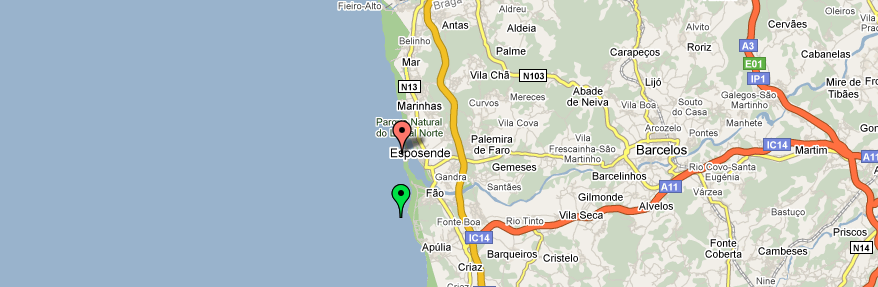
\includegraphics[width=\textwidth]{bilder/locate-esposende}
    \caption{Alternative Vorhersageposition für Esposende, Portugal}
    \label{locate-esposende}
  \end{center}
\end{figure}

\subsubsection{Verbesserung des Algorithmus}
Damit der Algorithmus für einen Spot auch wirklich die nächste
alternative Vorhersageposition findet, muss die Schrittweite $\delta$,
um die der Radius pro Iteration erhöht wird, sehr klein gewählt
werden. Ist diese Schrittweite zu groß, kann es vorkommen dass eine in
Wirklichkeit viel näher am Ursprung liegende alternative
Vorhersageposition nicht gefunden wird, da sie bei einer der
Iterationen übersprungen wurde. Wählt man die Schrittweite zu klein,
führt dies zu sehr vielen und teuren Aufrufen des Programms
\textit{degrib} und einer schlechten Laufzeit des
Algorithmus. Dasselbe gilt für die Wahl der Schrittweite $\alpha$, mit
der die verschiedenen Richtungen um die Ursprungsposition herum
berechnet werden. Um im Durchschnitt die Anzahl der \textit{degrib}
Programmaufrufe zu reduzieren, wurde hier ein Verfahren angewendet,
das dem einer binären Suche ähnelt und als \textit{Divide and Conquer}
Prinzip bekannt ist. Diese Variante des Algorithmus arbeitet
folgendermaßen:

\begin{enumerate}

\item Bei der Initialisierung wird wieder die maximale Distanz
  $\Delta$ festgelegt, die eine alternative Vorhersageposition von der
  Ursprungsposition eines Spots entfernt sein darf, und die
  Schrittweite $\alpha < 360^{\circ}$, mit der die Richtungen der zu
  untersuchenden Positionen berechnet werden. Außerdem wird ein
  Schwellenwert $d$ benötigt, der als Abbruchkriterium dient und im
  3. Schritt näher erklärt wird.

\item Da bei vielen Spots bereits an der Ursprungsposition
  Vorhersagedaten vorhanden sind, wird zunächst diese Position auf
  Gültigkeit überprüft. Wurde dort ein gültiger Vorhersagewert
  gefunden, kann die Ursprungsposition als Vorhersageposition
  verwendet werden und der Algorithmus ist fertig.

\item Falls nicht, wird in den nächsten beiden Schritten die
  alternative Vorhersageposition durch Anwendung des \textit{Divide
    and Conquer} Prinzips gesucht. Hierzu wird eine untere Schranke
  mit $l = 0$ und eine obere Schranke mit $u = \Delta$ festgelegt. Der
  Abstand der unteren und oberen Schranke wird in den folgenden
  Iterationen halbiert, bis dieser kleiner ist als der zuvor
  angegebene Schwellenwert $d$.

\item Mit dem Programm \textit{degrib} werden bestimmte Positionen auf
  gültige Vorhersagewerte hin überprüft, die auf dem Umkreis liegen,
  der durch den Radius $l + (u - l)/2$ definiert ist. Dabei werden
  wieder nur diejenigen Positionen betrachtet, deren in Grad
  angegebene Richtung durch die Schrittweise $\alpha$ teilbar ist.

  \begin{enumerate}

  \item Wurde auf dem Umkreis eine Position mit einem gültigen
    Vorhersagewert gefunden, wird diese als alternative
    Vorhersageposition vorgemerkt und die obere Schranke auf $u = u -
    (u - l)/2$ gesetzt.

  \item Wurde auf dem Umkreis keine Position mit gültigen
    Vorhersagewerten gefunden, wird die untere Schranke auf $l = l + (u -
    l)/2$ gesetzt.

  \end{enumerate}

\item Solange $u - l > d$ ist, wird mit Schritt 4
  weitergemacht. Ansonsten ist der Algorithmus fertig und die
  vorgemerkte Position kann als alternative Vorhersageposition
  verwendet werden. Wurde keine Position vorgemerkt, konnte der
  Algorithmus keine alternative Vorhersageposition finden und
  terminiert ohne Erfolg.

\end{enumerate}

\lstinputlisting[caption={Ausgabe bei der Suche einer alternativen
  Vorhersageposition},label=locate]{listings/locate.txt}

In Auflistung \ref{locate} ist die Ausgabe des Algorithmus für den
Spot Esposende in Portugal zu sehen. Der Algorithmus wurde mit einer
maximalen Distanz $\Delta$ von 100 Kilometern, einer
Richtungsschrittweite $\alpha$ von $10^{\circ}$ und einem
Schwellenwert $d$ von einem Meter initialisiert. Da an der
Ursprungsposition keine gültigen Vorhersagewerte gefunden wurden,
sucht der Algorithmus zunächst nach gültigen Position auf dem Umkreis
mit einem Radius von 50 Kilometern. In Zeile 2 kann man erkennen, dass
auf diesem Umkreis eine gültige Position gefunden wurde. Daher müssen
Positionen, die mehr als 50 Kilometer von der Ursprungsposition
entfernt sind, nicht weiter untersucht werden. In den folgenden
Iterationen werden weitere Positionen untersucht und die untere oder
obere Schranke entsprechend angepasst. Nachdem der Schwellenwert
unterschritten wurde, terminiert der Algorithmus nach ca. 8 Sekunden
mit einer alternativen Vorhersageposition, die 3,6 Kilometern weiter
südlich liegt.

\subsection{Transformation der Vorhersagedaten}
Nachdem die alternativen Vorhersagepositionen für das \textit{Wave
  Watch III} Modell ermittelt wurden, können die Vorhersagedaten der
Spots mit dem Programm \textit{degrib} ausgelesen und in das
\textit{CSV}-Format umgewandelt werden. Die Vorhersagedaten des
\textit{Wave Watch III} Modells werden dabei an der alternativen
Vorhersageposition, die Daten des \textit{Global Forecast System} an
der Ursprungsposition eines Spots ausgelesen. Hierzu wird das Programm
\textit{degrib} mit den entsprechenden Parametern pro Spot $n$-mal
aufgerufen, wobei $n$ für die Anzahl der Vorhersageelemente steht. Die
übergebenen Parameter sind der Name der \textit{Grib}-Datei und die
geographische Position, an der die Daten gelesen werden.

Die Ausgabe dieser Programmaufrufe entspricht der aus Auflistung
\ref{degrib} bekannten Struktur. Bis auf einige Feinheiten ist diese
Ausgabe schon fast in dem gewünschten \textit{CSV}-Format. Damit die
in der Ausgabe enthaltenen Zeitangaben vom \textit{Bulk} Loader des
Datenbankmanagementsystems interpretiert werden können, müssen diese
noch in ein durch \textit{ISO 8601} standardisiertes Datums- und
Zeitformat konvertiert werden. Zudem wird pro Datensatz noch der
Primärschlüssel des entsprechenden Spots hinzugefügt, damit die
Vorhersagedaten im späteren Ladevorgang eindeutig mit einem Spot in
Verbindung gebracht werden können. Das Ergebnis dieser Transformation
ist in Auflistung \ref{degrib-csv} zu sehen.

\lstinputlisting[caption={Vorhersagedaten aus Mundaka im CSV-Format},label=degrib-csv]{listings/degrib-csv.txt}

Der hier beschriebene Vorgang wird für alle Spots ausgeführt und die
Ausgabe der Transformation durch Anhängen in eine Datei
umgeleitet. Die so entstandene \textit{CSV}-Datei enthält schließlich
alle relevanten Vorhersagedaten in einem Format, das im nächsten
Schritt vom Bulk Loader des Datenbankmanagementsystem geladen werden
kann. Die \textit{Grib}-Dateien werden nach diesem Schritt nicht
weiter benötigt und können gelöscht werden.
\begin{table*}[h]
  \centering
  {\sf
    \footnotesize
    \begin{longtable}{c|c|c|c|c|c|c}

      \toprule
      \textbf{Element(e)} & \textbf{1 Spot} & \textbf{10 Spots} & \textbf{100 Sp.} & \textbf{1.000 Sp.} & \textbf{10.000 Sp.} & \textbf{100.000 Sp.} \\
      \midrule
      1 & 17 ms & 170 ms & 1,7 s & 17 s & 2 m 50 s & 28 m 20 s \\
      10 & 170 ms & 1,7 s & 17 s & 2 m 50 s & 28 m 20 s & 4 h 43 m \\
      \textbf{11} & \textbf{187 ms} &  \textbf{1,87 s} & \textbf{18,7 s} & \textbf{3 m 7 s} & \textbf{31 m 10 s} & \textbf{5 h 12 m} \\
      15 & 255 ms & 2,55 s & 25,5 s & 4 m 15 s & 42 m 30 s &  7 h 5 min\\
      \bottomrule
    \end{longtable}
  }

  \caption{Hochrechnung der Laufzeit des Transformationsvorgangs}
  \label{tab:transformation_laufzeit}

\end{table*}

Nach dem Erstellen der Indexstruktur dauert das Auslesen und die
Transformation der Vorhersagedaten für ein Element ca. 17
Millisekunden (ohne Index ca. 320 ms). In Tabelle
\ref{tab:transformation_laufzeit} ist eine Hochrechnung der Laufzeit
für mehrere Spots zu sehen. Wie viele Spots weltweit existieren
bzw. mit welcher Anzahl an zu verarbeitenden Spots zu rechnen ist,
kann an dieser Stelle nur geschätzt werden. Auf einer ähnlichen
Webseite \footnote{\url{http://www.wannasurf.com}} waren Mitte Oktober
2009 ungefähr 8.300 Spots weltweit gelistet. Das Auslesen der
Vorhersagedaten für 11 Elemente und deren Transformation in eine
\textit{CSV}-Datei würde für diese 8.300 Spots somit ca. 26 Minuten
dauern.

\subsection{Verbesserung des Transformationsvorgangs}
Sowohl hinsichtlich der Geschwindigkeit als auch der Korrektheit ist
das Auffinden der alternativen Vorhersageposition nicht optimal. Das
eigentlich zur Extraktion von Daten konzipierte Programm
\textit{degrib} wird hier ''missbraucht'', um eine Position zu finden,
an der Vorhersagedaten zur Verfügung stehen. Hierfür wird das Programm
mehrmals aufgerufen, um an verschiedenen Positionen Vorhersagedaten zu
extrahieren und diese auf Gültigkeit zu überprüfen. Diese vielen
Programmaufrufe könnten durch die Entwicklung geeigneter Routinen, die
direkt auf dem \textit{Grib} Format arbeiten, vermieden werden und
somit die Geschwindigkeit zum Auffinden der Vorhersageposition erhöht
werden. Da diese Position für jeden Spot allerdings nur einmalig
ermittelt werden muss, wurde dieser Weg hier erstmal nicht weiter
verfolgt.

Zudem stellt sich die Frage nach der optimalen Vorhersageposition. Da
der vorgestellte Algorithmus im Uhrzeigersinn sucht, wurde in
Abbildung \ref{locate-esposende} für Esposende, eine Position südlich
des eigentlichen Spots gefunden. Weiter westlich, auf gleicher Höhe
wie Esposende, sind allerdings auch Vorhersagedaten vorhanden. Welche
Position nun besser zur Extraktion der Vorhersagedaten geeignet ist
bzw. welche Vorhersagewerte am ehesten dem Spot entsprechen, müsste im
Detail noch untersucht werden. Die bisher erzielten Ergebnisse machen
jedoch einen realistischen Eindruck und liefern nachvollziehbare
Resultate, die als zufriedenstellend bewertet werden können.

Die Geschwindigkeit bei der Extraktion der Vorhersagedaten mit dem
Programm \textit{degrib} kann nicht bemängelt werden. Nachdem ein
Index erstellt wurde, ist ein schneller und wahlfreier Zugriff auf die
Daten einer \textit{Grib}-Datei möglich. Zwar wurde das Programm nicht
auf mögliche Optimierungen hin untersucht; es kann aber davon
ausgegangen werden, dass die Implementierung durch das
\textit{Meteorological Development Laboratory}
\footnote{\url{http://www.weather.gov/mdl}} sehr auf Effizienz
ausgerichtet ist. Stößt die Transformationsphase an ihre Grenzen,
würde sich eine parallele Verarbeitung der \textit{Grib}-Dateien
anbieten. Da die Transformationsphase eines Spots nicht von anderen
Spots abhängig ist, ist eine sequenzielle Verarbeitung nicht zwingend
erforderlich. Durch eine parallele Verarbeitung könnte die Performanz
der Transformationsphase erheblich verbessert werden und ein sehr viel
größerer Geschwindigkeitsvorteil erzielt werden, als dies mit
Optimierungen einer sequentiellen Verarbeitung möglich wäre. Das
Auslesen und die Transformation der Vorhersagedaten der 8.300 Spots
könnte man beispielsweise auf zwei Computern parallel durchführen, und
somit die bisher benötigte Zeit von 26 Minuten auf 13 Minuten
halbieren. Möglichkeiten zur parallelen Verarbeitung werden noch in
den Verbesserungsvorschlägen des Ladevorgangs vorgestellt, denen
deshalb hier nicht vorweggegriffen werden soll.

\section{Laden der Daten}
Die Aufgabe des Ladevorgangs besteht darin, die in den vorigen
Schritten erhobenen Vorhersagedaten in die operative Datenbasis der
Web-Applikation zu integrieren. Nachdem dieser Ladevorgang erfolgreich
abgeschlossen wurde, stehen der Web-Applikation die aktuellen
Vorhersagedaten zur Verfügung. 

\subsection{Datenbankschema der Vorhersagedaten}
Das Datenbankschema der Web-Applikation orientiert sich an den von
\textit{ActiveRecord} erwarteten Konventionen, die sich hier zum
Großteil auch bewährt haben. Beim Entwurf des Schemas wurden die
üblichen Methoden zur Normalisierung von Relationen angewendet,
Primär- und Fremdschlüssel definiert und Indizes zum schnelleren
Auffinden von Datensätzen erstellt. Da für die \textit{ETL}-Prozesse
nur zwei Tabellen von Interesse sind, wird hier auf die komplette
Darstellung des Datenbankschemas verzichtet und nur auf die für den
Ladevorgang relevanten Relationen eingegangen.

\subsubsection{Referenzielle Integrität in Ruby on Rails}
Seltsamerweise scheint in der \textit{Ruby on Rails} Community nicht
allzuviel Wert auf die \textit{ACID} \nomenclature{ACID}{Atomicity,
  Consistency, Isolation, Durability} Eigenschaften eines Datenbank
Management Systems gelegt zu werden. Nach fast 4 Jahren fehlen in der
\textit{API} von \textit{ActiveRecord} leider immer noch Methoden zur
Definition von Fremdschlüsseln. Auch in vielen Büchern und
Diskussionen zu \textit{Ruby on Rails} wird auf die Verwendung von
Fremdschlüsseln zur Sicherung der referenziellen Integrität nicht
eingegangen. Dieses Defizit wurde durch die Definition entsprechender
Methoden in der \textit{ActiveRecord} Bibliothek behoben, so dass
Fremdschlüssel direkt über die \textit{API} definiert werden
können. Diese stellen die referenzielle Integrität auf Datenbankebene
sicher. Bei der Entwicklung der Web-Applikation traten so einige
Fehler sehr viel schneller zum Vorschein, als wenn man darauf
verzichtet hätte.

\subsubsection{Repräsentation der Vorhersagedaten in der Datenbank}
Die Vorhersagedaten der Spots werden in einer Relation mit dem Namen
\textit{forecasts} gespeichert, deren Aufbau in Tabelle
\ref{tab:forecasts} zu sehen ist. Die Spalten der Tabelle enthalten
den Fremdschlüssel eines Spots, den Zeitpunkt der Vorhersage und die
Werte der Vorhersageelemente. Die Attribute
\textit{spot\textunderscore id} und \textit{valid\textunderscore time}
bilden den Schlüsselkandidaten der Relation. Pro Spot
(\textit{spot\textunderscore id}) existiert für jeden
Vorhersagezeitpunkt (\textit{valid\textunderscore time}) genau ein
Datensatz in der Tabelle. Um den \textit{ActiveRecord} Konventionen
gerecht zu werden und Datensätze dieser Tabelle aus anderen Tabellen
einfacher zu referenzieren, wird allerdings als künstlicher
Primärschlüssel das Attribut \textit{id} verwendet. Das Attribut
\textit{reference\textunderscore time} enthält den Zeitpunkt, an dem
die beiden Modelle erstellt wurden. Da das \textit{Global Forecast
  System} und das \textit{Wave Watch III} Modell im Moment zu den
selben Zeitpunkten erstellt wird, gilt dieses Attribut für beide
Modelle. Die beiden Attribute \textit{created\textunderscore at} und
\textit{updated\textunderscore at} sind zwei von \textit{ActiveRecord}
automatisch verwaltete Attribute, welche die Zeitpunkte an dem ein
Datensatz erstellt und an dem er zuletzt aktualisiert wurde,
enthalten. Alle anderen Attribute repräsentieren die
Vorhersageelemente der beiden Modelle und nehmen die mit
\textit{degrib} ausgelesenen Werte auf.

\begin{table*}[h]
  \centering
  {\sf
    \footnotesize
    \begin{longtable}{l|l|l}

      \toprule
      \textbf{Spaltenname} & \textbf{Datentyp} & \textbf{Modifikator} \\

      \midrule

      id & integer & not null default \\
      spot\textunderscore id & integer & not null \\
      reference\textunderscore time & timestamp with time zone & not null \\
      valid\textunderscore time & timestamp with time zone & not null \\
      significant\textunderscore wave\textunderscore height & double precision & - \\
      mean\textunderscore wave\textunderscore direction & double precision & - \\
      mean\textunderscore wave\textunderscore period & double precision & - \\
      peak\textunderscore wave\textunderscore direction & double precision & - \\
      peak\textunderscore wave\textunderscore period & double precision & - \\
      wind\textunderscore direction & double precision & - \\
      wind\textunderscore speed & double precision & - \\
      temperature & double precision & - \\
      total\textunderscore cloud\textunderscore cover & double precision & - \\
      precipitable\textunderscore water & double precision & - \\
      water\textunderscore equivalent\textunderscore snow\textunderscore depth & double precision & - \\
      created\textunderscore at & timestamp with time zone & not null \\
      updated\textunderscore at & timestamp with time zone & not null \\

      \bottomrule

    \end{longtable}
  }

  \caption{Schema der Datenbanktabelle \textit{forecasts}}
  \label{tab:forecasts}

\end{table*}

\subsection{Tupelorientierte Aktualisierung}
Eine offensichtliche Methode die Vorhersagedaten auf den neusten Stand
zu bringen, ist die \textit{tupelorientierte} Aktualisierung mit
\textit{SQL}. Tupelorientiert deshalb, weil für jedes Tupel, das in
die Zielrelation eingefügt bzw. dort aktualisiert wird, ein
\textit{SQL} Befehl ausgeführt wird.

Hierzu müsste man zunächst die Zeilen der \textit{CSV}-Datei zu
Datensätzen transformieren, die der Struktur der \textit{forecasts}
Relation entsprechen. Anschließend könnte man die zu aktualisierenden
Datensätze mit einem \textit{UPDATE} Befehl ändern und die neu
hinzugekommenen Datensätze mit einem \textit{INSERT} Befehl
einfügen. Bei einem Vorhersagezeitraum von 180 Stunden in einem 3
stündigen Intervall sind dies pro Spot $(180 / 3) + 1 = 61$
auszuführende \textit{SQL} Befehle, den Zeitpunkt der Analyse mit
berücksichtigt. Für die verwendeten 73 Spots wären das $61 * 73 =
4.453$, bei den zuvor erwähnten 8.300 Spots einer ähnlichen Webseite
$61 * 8.300 = 506.300$ auszuführende \textit{SQL} Befehle. Da sich bei
einer größeren Datenmenge der vom Datenbankmanagementsystem
betriebene Overhead beim Ausführen der vielen Befehle negativ auf die
Performanz des Ladevorgangs auswirkt \cite{postgresql:populate}, wurde
diese Methode zur Aktualisierung der Vorhersagedaten nicht weiter
verfolgt.

Das hier beschriebene Verfahren eignet sich für Anwendungen, bei denen
nur eine geringe Datenmenge zu verarbeiten und die Performanz des
Ladevorgangs nicht kritisch ist. Der Vorteil der tupelorientierten
Aktualisierung liegt in der Implementierung. Diese ist meist
verständlicher und einfacher, als auf Performanz getrimmte Varianten.

Bevor im nächsten Abschnitt ein aus dem Bereich des \textit{Data
  Warehousing} bekanntes Verfahren vorgestellt wird, sollen hier noch
einige Verbesserungsvorschläge gemacht werden. Um die Laufzeit einer
tupelorientierten Aktualisierung zu verbessern, sollte die
Dokumentation des verwendeten Datenbankmanagementsystems
herangezogen und mögliche Optimierungsvorschläge in Betracht gezogen
werden. Durch die Verwendung von \textit{Prepared Statements}, dem
Ausschalten der \textit{Auto-Commit} Einstellung und der Einbettung
aller Befehle in eine einzelne Transaktion kann die Performanz in
vielen Anwendungen gesteigert werden. Reichen diese Optimierungen
nicht aus, sind mit dem im folgenden Abschnitt beschriebenen Verfahren
sehr viel bessere Ergebnisse zu erzielen.

% Bei der Aktualisierung wird über die Datensätzen der \textit{CSV}
% Datei iteriert, und für jeden Datensatz ein \textit{UPDATE} Befehl,
% gefolgt von einem konditionalen \textit{INSERT} Befehl ausgeführt. Da
% für einen bestimmten Vorhersagezeitpunkt eines Spots bereits ein
% Datensatz aus einer früheren Modellberechnung existieren kann, wird
% zunächst ein \textit{UPDATE} Befehl ausgeführt. Durch die Angabe des
% Schlüsselkandidaten in der \textit{WHERE} Klausel des Befehls wird die
% Menge der zu aktualisierenden Datensätze auf genau einen
% beschränkt. Das Ergebnis des ausgeführten Befehls ist die Anzahl der
% aktualisierten Datensätze und beträgt entweder 0 oder 1. Wurde ein
% Datensatz geändert kann auf die folgende \textit{INSERT} Operation
% verzichtet, und mit dem nächsten Datensatz der \textit{CSV} Datei
% weitergemacht werden. Falls die \textit{UPDATE} Operation nicht
% erfolgreich war, wird der neue Datensatz mit einem \textit{INSERT}
% Befehl hinzugefügt. Nachdem alle Datensätze der Eingabe verarbeitet
% wurden ist die Zielrelation auf dem neusten Stand.

% \subsubsection{Abschätzung der auszuführenden Befehle}
% Sind in der \textit{CSV} Datei $n$ Datensätze enthalten, muss das
% Datenbankmanagementsystem im \textit{Worst-Case} Szenario $2 * n$ Befehle
% ausführen. Dieser Fall trifft allerdings nur dann zu, falls noch
% überhaupt keine Vorhersagedaten in der Datenbank enthalten sind. Da
% die Vorhersagezeitpunkte von zwei aufeinander folgenden
% Modellberechnungen immer nur um 6 Stunden \footnote{in einem
%   3-stündigen Vorhersageintervall} voneinander abweichen, reicht für
% die Mehrheit der Datensätze eine \textit{UPDATE} Operation aus. Eine
% zusätzliche \textit{INSERT} Operation ist nur für diejenigen
% Datensätze notwendig, die in dem abweichenden Zeitraum liegen. Da die
% Datensätze der \textit{CSV} Datei in der Reihenfolge Spot
% $\rightarrow$ Vorhersageelement $\rightarrow$ Vorhersagezeitpunkt
% sortiert sind, kann auf eine \textit{INSERT} Operation verzichtet
% werden, falls zuvor schon ein Datensatz für den entsprechenden Spot
% und den Vorhersagezeitpunkt bearbeitet wurde. Im Durchschnitt liegt
% die Anzahl der Befehle somit leicht über $n$. Die Anzahl der
% auszuführenden Befehle ist hier von der Zahl der Datensätze
% abhängig. Bei einer großen Datenmenge wirkt sich der vom Datenbankmanagementsystem
% betriebene Overhead beim Ausführen der vielen Befehle negativ auf die
% Performanz des Ladevorgangs aus.

\subsection{Bulk Loading}

Das grundlegende Problem der zuvor beschriebenen Methode besteht
darin, dass die abgesetzten \textit{SQL} Befehle tupelorientiert
arbeiten. Die \textit{SQL} Befehle zur Manipulation von Datensätzen
können aber auch mengenorientiert eingesetzt werden, so dass pro
Befehl mehrere Tupel geändert bzw. hinzugefügt werden. Voraussetzung
hierfür ist, dass das Datenbankmanagementsystem auf alle zu
verarbeitenden Daten zugreifen kann. Dies war bei der vorigen Methode
nicht der Fall, da das Datenbankmanagementsystem bei jeder Operation
nur einen Datensatz der Eingabe zu Gesicht bekam.

In diesem Abschnitt wird beschrieben wie die Vorhersagedaten der
\textit{CSV}-Datei effizient unter die Kontrolle des Datenbank
Management Systems gebracht werden können. Die Daten werden zunächst
in einen temporären Bereich der Datenbank geladen, der sogenannte
\textit{Staging Area}. Von dort aus werden sie in einem weiteren
Schritt in die operative Datenbasis der Web-Applikation überführt. Die
hier verwendete \textit{Staging Area} besteht aus einer einzigen, in
Tabelle \ref{tab:grib_messages} zu sehenden, Relation, deren Attribute
die Spalten der \textit{CSV}-Datei widerspiegeln.

\begin{table*}[h]
  \centering
  {\sf
    \footnotesize
    \begin{longtable}{l|l|l}

      \toprule
      \textbf{Spaltenname} & \textbf{Datentyp} & \textbf{Modifikator} \\

      \midrule
      id & integer & not null default  \\
      spot\textunderscore id & integer & not null \\
      latitude & double precision & not null \\
      longitude & double precision & not null \\
      element & character varying(255) & not null \\
      unit & character varying(255) & not null \\
      reference\textunderscore time & timestamp with time zone & not null \\
      valid\textunderscore time & timestamp with time zone & not null \\
      value & double precision & - \\

      \bottomrule

    \end{longtable}
  }

  \caption{Schema der Datenbanktabelle \textit{grib\textunderscore messages}}
  \label{tab:grib_messages}

\end{table*}

Bevor die Daten in diese Tabelle geladen werden, wird diese zunächst
von den Datensätzen eines vorherigen Ladevorgangs
bereinigt. Anschließend könnten die Vorhersagedaten mit
\textit{INSERT} Operationen in diese Relation eingefügt werden. Auch
hier würde sich die Verwendung eines \textit{Prepared Statement}
anbieten, da eine hohe Anzahl sich ähnelnder Befehle verarbeitet
werden müsste. Im Bereich des \textit{Data Warehousing} wird beim
Laden von Daten allerdings immer auf die sogenannten \textit{Bulk
  Loader} der verwendeten Datenbankmanagementsysteme verwiesen. Dies
sind meist datenbankspezifische Befehle oder Programme, mit denen
größere Datenmengen effizienter als mit den standardisierten
\textit{SQL} Befehlen geladen werden können. Der \textit{Bulk Loader}
von \textit{PostgreSQL} ist durch die \textit{COPY} Befehlsfamilie
implementiert, mit der Daten im Text-, \textit{CSV-} oder Binärformat
importiert und exportiert werden können. Der Befehl aus Auflistung
\ref{lst:copy} veranlasst \textit{PostgreSQL} dazu, die über den
Standard Eingabekanal gelesenen Datensätze in die Tabelle
\textit{grib\textunderscore messages} zu importieren. Dieser Befehl
wird mit \textit{PostgreSQL}'s Kommandozeilenprogramm \textit{psql}
ausgeführt und die Datensätze der \textit{CSV}-Datei über den Standard
Eingabekanal weitergereicht. Nachdem mit dem \textit{COPY} Befehl alle
Daten geladen wurden, wird ein zusätzlicher \textit{ANALYZE} Befehl
ausgeführt, der die Statistiken der Tabelle aktualisiert, die vom
Anfrageoptimierer des Datenbankmanagementsystems verwendet werden,
um einen guten Ausführungsplan zu finden.

\begin{lstlisting}[captionpos=b, caption=Befehl zum Import von Datensätzen in \textit{PostgreSQL}, label=lst:copy]
COPY grib_messages (
  spot_id, latitude, longitude, element, unit, 
  reference_time, valid_time, value
) FROM STDIN;
\end{lstlisting}

Im Abschnitt \textit{Populating a Database} \cite{postgresql:populate}
der \textit{PostgreSQL} Dokumentation sind weitere nützliche Hinweise
zu finden, die beim Verarbeiten größerer Datenmengen zu beachten
sind. Auf der Zielrelation definierte Indizes, \textit{Check
  Constraints} und \textit{Trigger}, wirken sich negativ auf die
Performanz des Ladevorgangs aus. Hier wird zum Beispiel vorgeschlagen,
auf der Zielrelation definierte Indizes vor dem Laden zu entfernen und
anschließend wieder neu zu erstellen. Die Konfiguration des Datenbank
Management Systems selbst ist auch nicht außer Acht zu lassen. Die
Performanz von PostgreSQL lässt sich durch das Einstellen bestimmter
Parametern in der Konfigurationsdatei verbessern, da die Standard
Werte in einigen Distributionen für heutige Hardware relativ niedrig
angesetzt sind. Eine optimale Systemkonfiguration benötigt allerdings
einiges an Erfahrung und Geduld beim Ausprobieren der verschiedenen
Konfigurationsparameter.

\subsection{Mengenorientierte Aktualisierung}
Nachdem die zu verarbeitenden Daten unter die Kontrolle des Datenbank
Management Systems gebracht wurden, kann mit der mengenorientierten
Aktualisierung der Vorhersagedaten begonnen werden. Ziel ist, die
Vorhersagedaten der Relation \textit{grib\textunderscore messages} in
die Relation \textit{forecasts} zu überführen. Dabei werden
existierende, aus einer früheren Modellberechnung stammenden
Datensätze der Tabelle \textit{forecasts} mit den Werten der neueren
Berechnung überschrieben und noch nicht existierende Datensätze
hinzugefügt. Es werden nur diejenigen Datensätze aktualisiert bzw.
hinzugefügt, die auch im Zeitraum der aktuellen Modellberechnung
liegen. Dieser Zeitraum ist durch die Datensätze der Quellrelation
\textit{grib\textunderscore messages} bestimmt und kann mit dem
\textit{SQL} Befehl \textit{SELECT MIN(valid\textunderscore time),
  MAX(valid\textunderscore time) FROM grib\textunderscore messages}
ermittelt werden.

\subsubsection{Transposition von Spalten und Zeilen}
Idealerweise würde man bei der mengenorientierten Aktualisierung genau
zwei Befehle ausführen. Ein \textit{UPDATE} Befehl, der alle
existierenden Datensätze der \textit{forecasts} Relation aktualisiert
und ein \textit{INSERT} Befehl, mit dem neue Datensätze hinzugefügt
werden. Die Art und Weise wie die Daten aber in der Relation
\textit{grib\textunderscore messages} vorliegen, würde zu sehr
komplexen \textit{SQL} Befehlen oder dem Einsatz datenbankspezifischer
Erweiterungen führen. Das Problem besteht darin, dass mehrere
Datensätze der Relation \textit{grib\textunderscore messages} zu einem
Datensatz der Relation \textit{forecasts} überführt werden
müssen. Oder anders ausgedrückt: Die Zeilen der Quellrelation müssen
zu Spalten der Zielrelation transponiert werden. Die Konstruktion
solcher Anfragen lässt sich nur umständlich in \textit{SQL} ausdrücken
und führt üblicherweise zu sehr komplexen Befehlen, deren Performanz
sich gegenüber anderer Alternativen anzweifeln lässt. Für diese Art
von Anfragen werden in \textit{PostgreSQL} üblicherweise die
sogenannten \textit{crosstab} Funktionen aus dem \textit{tablefunc}
Modul verwendet. Da bei einem Engpass des Ladevorgangs allerdings eine
Vorverarbeitung der \textit{CSV}-Datei mit \textit{awk} und ähnlichen
Programmen als vielversprechender angesehen wird, wurde diese
Alternativen hier nicht weiter verfolgt, sondern eine inkrementelle
und zugleich einfachere Strategie gewählt.

\subsubsection{Hinzufügen von Datensätzen}
Die gewählte Strategie zur Aktualisierung der Vorhersagedaten erfolgt
in zwei Schritten. Im ersten Schritt wird durch das Hinzufügen
entsprechender Datensätze sichergestellt, dass für jeden Spot und
jeden Vorhersagezeitpunkt der Quellrelation ein Datensatz in der
Zielrelation existiert. Diese hinzugefügten Datensätze dienen als
Platzhalter und werden im zweiten Schritt mit den Vorhersagedaten der
Quellrelation aktualisiert. Mit einer \textit{SQL} Anfrage wird
diejenige Menge an Datensätze erzeugt, deren Schlüsselkandidaten noch
nicht in der Zielrelation existieren, sich aber aus den Datensätzen
der Quellrelation ableiten lassen. Diese Datensätze dienen
vorübergehend als Platzhalter und enthalten nur gültige Werte in den
Attributen \textit{spot\textunderscore id},
\textit{valid\textunderscore time}, \textit{created\textunderscore
  at}, \textit{updated\textunderscore at} und
\textit{reference\textunderscore time}. Alle anderen Attribute
repräsentieren die Vorhersageelemente und werden mit dem Wert
\textit{NULL} belegt. Diese Platzhalter Datensätze werden durch einen
\textit{INSERT} Befehl in die Tabelle \textit{forecasts} eingefügt.

\subsubsection{Beeinflussung des Anfrageoptimierers}
Die Menge der hinzuzufügenden Datensätze kann durch Verwendung
verschiedenster \textit{SQL} Konstrukte erzeugt werden. Eine der
Aufgaben des Datenbankmanagementsystems besteht darin, einen guten
Ausführungsplan für eine Anfrage zu finden. Idealerweise sollten dabei
zwei äquivalente Befehle in den optimalen Ausführungsplan übersetzt
werden. Diese komplexe Aufgabe wird von den Optimierern der
verschiedenen Datenbankmanagementsysteme allerdings unterschiedlich
gut gelöst. Durch das Verwenden verschiedener \textit{SQL} Konstrukte
kann der Optimierer eines Datenbankmanagementsystems teilweise
beeinflusst werden. Hier wurde das Laufzeitverhalten von zwei
äquivalenten \textit{SQL} Befehlen durch die Analyse ihrer
Ausführungspläne untersucht. Beide Befehle wurden auf einer Datenbank
ausgeführt, in der 32452 Datensätze in der Relation
\textit{grib\textunderscore messages} enthalten waren. Diese
Datensätze repräsentierten die Vorhersagedaten für 78 Spots über einen
Zeitraum von ca. 4 Monaten. Der erste Befehl verwendet einen
sogenannten \textit{Left Join} um das Ergebnis zu berechnen, im
zweiten Befehl wird eine \textit{Subquery} benutzt.

\subsubsection{Analyse der Ausführungspläne}
Da der Optimierer von \textit{PostgreSQL} bei der Wahl des
Ausführungsplans Statistiken über Tabellen verwendet, ist es wichtig,
diese regelmäßig zu aktualisieren. Üblicherweise wird dies in einem
bestimmten Intervall durch einen Hintergrundprozess erledigt, sollte
aber nach dem Einfügen oder Entfernen von vielen Datensätzen manuell
mit dem \textit{ANALYZE} Befehl durchgeführt werden. Um den
Ausführunsplan eines \textit{SQL} Befehls in \textit{PostgreSQL}
anzuzeigen, wird der \textit{EXPLAIN} Befehl benutzt. Durch die Angabe
der \textit{ANALYZE} Option wird der zu untersuchende Befehl
ausgeführt und Informationen über dessen Laufzeit ausgegeben. Die hier
gezeigten Ausführungspläne wurden zwar mit der \textit{ANALYZE} Option
erstellt, enthalten der Übersichtlichkeit halber aber nicht alle
Informationen. Vor der Analyse der Ausführungspläne wurden auf allen
Attributen, die in Anfragen referenziert werden, Indizes definiert und
die Statistiken der Tabellen aktualisiert. Auf den Schlüsselkandidaten
\textit{spot\textunderscore id} und \textit{valid\textunderscore time}
wurden zusätzlich noch zusammengesetzte Indizes definiert.

\subsubsection{Ausführungsplan der Left Join Anfrage}
In Auflistung \ref{forecasts:insert_1} ist der \textit{SQL} Befehl als
\textit{Left Join} Variante zu sehen, mit der die Menge der
hinzuzufügenden Datensätze erzeugt wird. Der Befehl verknüpft die
Datensätze der Relation \textit{grib\textunderscore messages} über die
Attribute \textit{spot\textunderscore id} und
\textit{valid\textunderscore time} mit den Datensätzen der Relation
\textit{forecasts}. Durch die Bedingung in der \textit{WHERE} Klausel
wird das Ergebnis auf diejenigen Datensätze reduziert, deren
Schlüsselkandidat noch nicht in der Relation \textit{forecasts}
existiert. Dies sind genau die Vorhersagezeitpunkte, die seit der
letzten Modellberechnung neu hinzugekommen sind.

\begin{lstlisting}[captionpos=b, caption=Hinzufügen von Datensätze mittels Left Join, label=forecasts:insert_1, language=SQL]
INSERT INTO forecasts(spot_id, valid_time, created_at, updated_at, 
                      reference_time)
     SELECT grib_messages.spot_id, grib_messages.valid_time, 
            NOW() AT TIME ZONE 'UTC', NOW() AT TIME ZONE 'UTC', 
            MAX(grib_messages.reference_time)
       FROM grib_messages
  LEFT JOIN forecasts
         ON forecasts.spot_id = grib_messages.spot_id
        AND forecasts.valid_time = grib_messages.valid_time
      WHERE forecasts.id IS NULL
   GROUP BY grib_messages.spot_id, grib_messages.valid_time;
\end{lstlisting}

Obwohl auf den entsprechenden Attributen beider Relationen Indizes
definiert sind, kann man im Ausführungsplan in Auflistung
\ref{forecasts:explain_1} sehen, dass kein einziger Index benutzt
wird, sondern ein \textit{Sequence Scan} auf den beiden Relationen
\textit{forecasts} und \textit{grib\textunderscore messages}
durchgeführt wird. Falls viele Spots hinzukommen oder historische
Vorhersagedaten für statistische Zwecke und \textit{Data Mining}
Verfahren über einen längeren Zeitraum behalten werden, könnte man
hier auf Dauer Probleme bekommen. Der Optimierer scheint bei dieser
Anfrage nicht zu erkennen, dass die Ergebnismenge im Vergleich zu der
Anzahl von Datensätzen in der \textit{forecasts} Relation sehr gering
ist. Im Ergebnis befinden sich nämlich nur diejenigen Datensätze, die
seit der letzten Modellberechnung hinzugekommen sind. Das Problem
liegt hier in der Verwendung des \textit{Left Joins}, der den
Optimierer dazu veranlasst, alle Datensätze der beiden Relationen zu
verknüpfen und erst anschließend den Großteil der Datensätze wieder
weg zu werfen.

\begin{lstlisting}[captionpos=b, caption=Ausführungsplan des Left Joins, label=forecasts:explain_1]
GroupAggregate (cost=14275.00..15496.03 rows=3246 width=20)
 Merge Left Join (cost=14275.00..15317.53 rows=16226 width=20)
   Merge Cond: ((grib_messages.spot_id = forecasts.spot_id) AND 
                (grib_messages.valid_time = forecasts.valid_time))
   Filter: (forecasts.id IS NULL)
     Sort (cost=3778.65..3859.78 rows=32452 width=20)
       Sort Key: grib_messages.spot_id, grib_messages.valid_time
         Seq Scan on grib_messages  (cost=0.00..678.52 rows=32452 width=20)
     Materialize (cost=10496.30..11300.77 rows=64358 width=16)
       Sort (cost=10496.30..10657.19 rows=64358 width=16)
         Sort Key: forecasts.spot_id, forecasts.valid_time
           Seq Scan on forecasts  (cost=0.00..4253.58 rows=64358 width=16)
Total runtime: 213.518 ms
\end{lstlisting}

Die auf beiden Relationen definierten Indizes erweisen sich bei dieser
Anfrage als nutzlos. Der Optimierer von \textit{PostgreSQL} kann durch
das Setzen entsprechender Parameter allerdings beeinflusst werden. Die
Ausführung des selben Befehls mit einem erzwungenen \textit{Index
  Scan} ergab ein sehr viel schlechteres Ergebnis als der im
Allgemeinen als negativ bewertete \textit{Sequence Scan}. Das Problem
dieser Anfrage lässt sich also nicht durch die geschickte Definition
von Indizes lösen, sondern durch die Vermeidung des \textit{Left
  Joins}.

Nichtsdestotrotz traten bei der Verwendung dieses Befehls über einen
Zeitraum von ca. 3 Monaten hinweg keine Probleme auf. Der Befehl wurde
alle 4 Stunden durch einen \textit{Cronjob} ausgeführt und provozierte
dabei keinerlei Auffälligkeiten. Die Ausführungszeit beträgt bei der
jetzigen Datenmenge ca. 214 Millisekunden und kann als akzeptabel
angesehen werden. Die Ausführungszeit wird aber mit einem Anwachsen
der \textit{forecasts} Relation stetig zunehmen. Eine bessere
Alternative ist, die Anfrage in eine \textit{Subquery} umzuformen.

\subsubsection{Ausführungsplan der Subquery Anfrage}
Ein äquivalenter Befehl zum Einfügen der Platzhalter Datensätze ist in
Auflistung \ref{forecasts:insert_2} zu sehen. Bei dieser Variante wird
eine \textit{korrelierte Subquery} verwendet, die im Allgemeinen als
kritisch hinsichtlich der Performanz eingestuft wird. Bei einer
\textit{korrelierten Subquery} werden in der inneren Anfrage Attribute
der Äußeren referenziert, was bei der Ausführung dazu führt, dass die
innere Anfrage für jeden Datensatz ausgeführt werden muss, der durch
die Äußere erzeugt wird.

\begin{lstlisting}[captionpos=b, caption=Hinzufügen von Datensätzen mittels Subquery, label=forecasts:insert_2, language=SQL]
INSERT INTO forecasts(spot_id, valid_time, created_at, updated_at, 
                      reference_time)
     SELECT grib_messages.spot_id, grib_messages.valid_time, 
            NOW() AT TIME ZONE 'UTC', NOW() AT TIME ZONE 'UTC', 
            MAX(grib_messages.reference_time)
       FROM grib_messages
      WHERE NOT EXISTS (
              SELECT 1 
                FROM forecasts 
               WHERE forecasts.spot_id = grib_messages.spot_id
                 AND forecasts.valid_time = grib_messages.valid_time)
   GROUP BY grib_messages.spot_id, grib_messages.valid_time;
\end{lstlisting}

Wie man aber am Ausführungsplan aus Auflistung
\ref{forecasts:explain_2} erkennen kann, ist diese Anfrage mit ca. 100
Millisekunden jedoch doppelt so schnell wie die eben untersuchte
\textit{Left Join} Variante. Der \textit{Sequence Scan} auf der
\textit{grib\textunderscore messages} Relation ist hier kein Problem,
da ohnehin alle Datensätze dieser Relation betrachtet werden müssen,
um das Ergebnis zu berechnen. Der teure \textit{Sequence Scan} auf der
Relation \textit{forecasts} konnte hier jedoch vermieden
werden. Stattdessen wird für jeden Datensatz aus der Tabelle
\textit{grib\textunderscore messages} der zusammengesetzte Index auf
dem Schlüsselkandidaten benutzt, um die Existenz eines entsprechenden
Datensatzes in der Tabelle \textit{forecasts} zu überprüfen.

\begin{lstlisting}[captionpos=b, caption=Ausführungsplan der Subquery, label=forecasts:explain_2]
Subquery Scan "*SELECT*"  (cost=270420.52..270481.38 rows=1623 width=36)
 HashAggregate (cost=270420.52..270448.92 rows=1623 width=20)
  Seq Scan on grib_messages  (cost=0.00..270298.82 rows=16226 width=20)
   Filter: (NOT (subplan))
    SubPlan
     Index Scan using index_forecasts_on_spot_id_and_valid_time 
                      on forecasts (cost=0.00..8.31 rows=1 width=0)
      Index Cond: ((spot_id = $0) AND (valid_time = $1))
Total runtime: 98.575 ms
\end{lstlisting}

Die Performanz der \textit{Subquery} Variante wird bei einer Zunahme
von Datensätzen der \textit{forecasts} Relation nur minimal
beeinflusst, da die Anzahl der \textit{Subquery} Aufrufe durch die
Zahl der Datensätze in der Tabelle \textit{grib\textunderscore
  messages} beschränkt ist. Die Größe der \textit{forecasts} Relation
kann sich hier nur beim Auffinden von Datensätze über den stetig
wachsenden Index negativ auswirken. Diese Beeinflussung ist allerdings
gerade wegen der Verwendung geeigneter Indexstrukturen so gering, dass
sie hier vernachlässigt werden kann.

Zusammenfassend kann man zu dieser Untersuchung sagen, dass durch die
Wahl entsprechender \textit{SQL} Konstrukte der Anfrageoptimierer
eines Datenbankmanagementsystems beeinflusst werden kann und sich
dies auf die Performanz der Anfrage auswirken kann. Dies spielt bei
der hier zu Analysezwecken verwendeten Datenmenge zwar noch keine
große Rolle, kann bei einer größeren Datenmengen aber fatale
Auswirkungen auf die Laufzeit der Anfragen haben. Wie man sehen
konnte, war die \textit{Subquery} Anfrage im Gegensatz zur
\textit{Left Join} Anfrage durch die Anzahl der Datensätze in der
Tabelle \textit{grib\textunderscore messages} beschränkt. Diese
Beschränkung ist wiederum abhängig von der Anzahl der Spots, was auch
genau so sein sollte. Wichtig ist hier nicht, dass die Laufzeit um das
doppelte beschleunigt wurde, sondern dass die Anfrage durch die Anzahl
der Spots und nicht durch die Anzahl der historischen Daten beschränkt
ist.

\subsubsection{Aktualisierung der Vorhersagedaten}
Die Aktualisierung der Vorhersagedaten wird wegen der erwähnten
Transposition von Zeilen zu Spalten elementweise durchgeführt. Für
jedes Vorhersageelement wird ein \textit{UPDATE} Befehl ausgeführt,
der die entsprechende Spalte der Datensätze aus der \textit{forecasts}
Relation aktualisiert. In Auflistung \ref{forecasts:update} ist der
\textit{UPDATE} Befehl zu sehen, mit dem die Wellenhöhen aktualisiert
werden. Da sich die Befehle nur in der Angabe des Spaltennamen in
Zeile 3 und der Angabe der Elementkennung in Zeile 6 unterscheiden,
werden diese Befehle dynamisch erzeugt und hintereinander ausgeführt.

\begin{lstlisting}[captionpos=b, caption=Aktualisierung der Wellenhöhe, label=forecasts:update, language=SQL]
UPDATE forecasts
   SET reference_time = grib_messages.reference_time,
       significant_wave_height = grib_messages.value,
       updated_at = NOW() AT TIME ZONE 'UTC'
  FROM grib_messages
 WHERE grib_messages.element = 'HTSGW'
   AND grib_messages.spot_id = forecasts.spot_id
   AND grib_messages.valid_time = forecasts.valid_time;
\end{lstlisting}

Der Ausführungsplan in Auflistung \ref{forecasts:update_explain}
zeigt, dass bei der Aktualisierung zwei Indizes genutzt werden. Zum
einen wird der Index auf dem Attribut \textit{element} der Tabelle
\textit{grib\textunderscore messages} genutzt, um nur diejenigen
Zeilen zu finden, in denen die Wellenhöhe gespeichert ist. Zum anderen
wird der zusammengesetzte Index auf dem Schlüsselkandidaten der
Tabelle \textit{forecasts} beansprucht, um nur Vorhersagen zu
aktualisieren, die auch im Zeitraum der aktuellen Modellberechnung
liegen. Die Laufzeit zur Aktualisierung der Wellenhöhe beträgt ca. 108
Millisekunden und ist wegen der Verwendung des Index auf der Tabelle
\textit{forecasts} ebenfalls durch die Anzahl der Spots
beschränkt. Die Laufzeit der \textit{UPDATE} Befehle zur
Aktualisierung der anderen Vorhersagespalten verhält sich ähnlich.

\begin{lstlisting}[captionpos=b, caption=Ausführungsplan der Aktualisierung, label=forecasts:update_explain]
Nested Loop (cost=108.56..17995.79 rows=4619 width=134)
  Bitmap Heap Scan on grib_messages (cost=108.56..521.11 rows=4684 width=28)
    Recheck Cond: ((element)::text = 'HTSGW'::text)
      Bitmap Index Scan on index_grib_messages_on_element  
                           (cost=0.00..107.38 rows=4684 width=0)
        Index Cond: ((element)::text = 'HTSGW'::text)
  Index Scan using index_forecasts_on_spot_id_and_valid_time on forecasts 
                   (cost=0.00..3.71 rows=1 width=118)
    Index Cond: ((forecasts.spot_id = grib_messages.spot_id) AND 
                 (forecasts.valid_time = grib_messages.valid_time))
Total runtime: 107.865 ms
\end{lstlisting}

Bei der mengenorientierten Aktualisierung der Vorhersagedaten werden
insgesamt \textit{N+1} Anfragen ausgeführt, wobei \textit{N} für die
Anzahl der Vorhersageelemente steht. Zunächst wird ein \textit{INSERT}
Befehl ausgeführt und anschließend ein \textit{UPDATE} Befehl pro
Vorhersageelement. Alle Befehle zur Aktualisierung der Vorhersagedaten
laufen in einer Transaktion ab, durch die sichergestellt ist, dass der
ursprünglichen Status der Datenbank bei einem eventuellen Fehler
wieder hergestellt wird. Die Angaben zur Laufzeit der \textit{SQL}
Befehle schwanken im Bereich von ca. 50 Millisekunden und können auch
nur als grobe Richtwerte für die hier verwendete Datenmenge verstanden
werden. Diese Schwankungen haben unter anderem mit dem Cache des
Datenbankmanagementsystems zu tun.

\subsubsection{Laufzeitverhalten bei einer größeren Datenmenge}
Eine konkrete Aussage über die Laufzeit des Ladevorgangs bei einer
höheren Anzahl von Spots zu machen, ist schwer. Dies liegt
hauptsächlich darin begründet, dass nicht bekannt ist, wie sich der
Anfrageoptimierer und die Laufzeit der einzelnen Befehle bei einer
größeren Datenmenge verhalten. Kommen mehr Daten hinzu, verändern sich
die Statistiken, die vom Anfrageoptimierer dazu verwendet werden,
einen geeigneten Ausführungsplan zu finden. Durch die Anpassung von
Parametern zur Konfiguration des Datenbankmanagementsystems kann das
Verhalten des Anfrageoptimierers ebenfalls beeinflusst werden. Diese
Parameter hängen wiederum von den Eigenschaften der verwendeten
Hardware ab. Eine Diskussion zur optimalen Einstellung von
Konfigurationsparametern würde zum einen den Rahmen dieser Arbeit
sprengen, zum anderen der Aussage \textit{''Premature optimization is
  the root of all evil''} von
\footnote{\url{http://shreevatsa.wordpress.com/2008/05/16/premature-optimization-is-the-root-of-all-evil}}
Donald Knuth widersprechen. Da bisher noch kein Engpass existiert,
wurden in diese Richtung hin keine weiteren Untersuchen gemacht.

Um trotzdem ein gewisses Gefühl für die Laufzeit bei einer höheren
Anzahl von Spots zu bekommen, wird hier eine Hochrechnung der Laufzeit
vorgestellt, die auf vereinfachten Annahmen basiert. Da die Laufzeit
der einzelnen Befehle sich in einem ähnlichen Zeitrahmen bewegen, wird
hier die Annahme getroffen, dass die Laufzeit eines einzelnen Befehls
konstant ist und sich aufsummieren lässt. Weiterhin wird angenommen,
dass sich die Laufzeit bei einer Zunahme der Datenmenge nicht
verändert. Somit kann die Gesamtlaufzeit der \textit{SQL} Befehle für
einen Spot mit $L = ((N+1) * l) / 78$ abgeschätzt werden, wobei $N$
für die Anzahl der Vorhersageelemente, $l$ für die Laufzeit eines
\textit{SQL} Befehls und 78 für die Anzahl der Spots steht, die bei
der zuvor durchgeführten Untersuchung existierten. Die Werte in
Tabelle \ref{tab:sql_laufzeit} wurden unter der Annahme berechnet,
dass $N=11$ Vorhersageelemente für jeden Spot verarbeitet werden.

\begin{table*}[h]
  \centering
  {\sf
    \footnotesize
    \begin{longtable}{l|c|c|c|c|c}

      \toprule
      \textbf{Laufzeit} & \textbf{1 Spot} & \textbf{100 Spots} & \textbf{1.000 Spots} & \textbf{10.000 Spots} & \textbf{100.000 Spots} \\
      \midrule
      $l$ = 200 ms & 31 ms & 3,1 s & 31 s &  5m 10 s &  51 m 40 s \\
      $l$ = 400 ms & 62 ms & 6,2 s & 1 m 2 s & 10 m 20 s & 1 h 43 m \\
      $l$ = 600 ms & 92 ms & 9,2 s & 1 m 32 s & 15 m 20 s & 2 h 33 m \\
      \bottomrule

    \end{longtable}
  }

  \caption{Hochrechnung der Laufzeit aller \textit{SQL} Befehle}
  \label{tab:sql_laufzeit}

\end{table*}

Wie nahe die hier vorgestellte Hochrechnung an der Realität ist,
bleibt allerdings offen. Da davon ausgegangen wird, dass die Laufzeit
$l$ eines einzelnen Befehls bei Zunahme der Datenmenge ebenfalls
steigt, würden in der Realität wohl eher schlechtere Ergebnisse als in
Tabelle \ref{tab:sql_laufzeit} erzielt werden.

\subsection{Verbesserung des Ladevorgangs}
Das Laden der Vorhersagedaten mit dem \textit{Bulk Loader} von
\textit{PostgreSQL} wird als unproblematisch angesehen. Im Abschnitt
''\textit{Performance Tips}'' \cite{postgresql:performance} der
\textit{PostgreSQL} Dokumentation werden einige Vorschläge gemacht,
die zur Steigerung der Performanz beitragen können. Beispielsweise
kann der \textit{COPY} Befehl am schnellsten ausgeführt werden, wenn
er in der selben Transaktion wie ein zuvor abgesetzter \textit{CREATE
  TABLE} oder \textit{TRUNCATE} Befehl ausgeführt wird. In diesem Fall
kann auf das sonst zu verwaltende \textit{Write Ahead Log} verzichtet
werden, da bei einem Fehler die Daten wieder gelöscht
werden. Weiterhin wird vorgeschlagen, die Indizes einer zu ladenden
Tabelle vor dem Laden zu löschen und erst danach wieder zu erstellen,
da der Aufbau eines neuen Index schneller ist als eine zeilenweise
Aktualisierung. Bei der jetzigen Datenmenge wird der Umsetzung dieser
Verbesserungsvorschläge allerdings eine eher geringe Priorität
eingeräumt, da der zu erzielende Geschwindigkeitsvorteil im Vergleich
zu anderen Vorschlägen als nicht sehr hoch eingestuft wird.

Viel mehr Potential zur Beschleunigung des Ladevorgangs wird in einer
Vorverarbeitung der Vorhersagedaten gesehen. Durch diesen zusätzlichen
Schritt könnte man die Vorhersagedaten in eine \textit{CSV}-Datei
transformieren, die der Struktur der \textit{forecasts} Tabelle
entspricht. Die bisher in der Datenbank durchgeführte Transposition
von Zeilen zu Spalten würde so in ein externes Programm verlagert
werden, mit der Aussicht, diese effizienter durchführen zu können, als
dies mit den Boardmitteln des Datenbankmanagementsystems möglich
ist. Die transformierte Datei kann dann in eine entsprechende
\textit{Staging Area} geladen werden und mit einem \textit{UPDATE-}
und einem \textit{INSERT} Befehl in die \textit{forecasts} Relation
integriert werden. Eine noch bessere Alternative wäre, die zu
aktualisierenden Datensätze der \textit{forecasts} Tabelle vor dem
Laden zu löschen und die \textit{CSV}-Datei mit einem \textit{COPY}
Befehl direkt in diese Relation zu integrieren. Ein Nachteil an diesem
Vorschlag ist, dass der Transformationsschritt vom
Aktualisierungszeitplan der beiden Modelle abhängig ist. Da die Daten
beider Modelle zu einem Datensatz der \textit{forecasts} Relation
transformiert werden, stellt sich die Frage, welche Strategie man bei
der Transformation und beim späteren Laden wählt, falls die Modelle
erst zu unterschiedlichen Zeitpunkten zur Verfügung stehen (was in der
Regel der Fall ist). Hier wäre die einfachste Möglichkeit, den
Transformationsschritt erst dann anzustoßen, wenn die Daten beider
Modelle verfügbar sind. Andernfalls müsste man die aktuellen Daten des
einen Modells mit den schon geladenen Daten des anderen Modells
verknüpfen.

\begin{table*}[h]
  \centering
  {\sf
    \footnotesize
    \begin{longtable}{l|c|c|c|c}

      \toprule
      \textbf{Phase} & \textbf{100 Spots} & \textbf{1.000 Spots} & \textbf{10.000 Spots} & \textbf{100.000 Spots}\\
      \midrule
      Extraktion \textit{(NWW3)} & 4 m & 4 m & 4 m & 4 m \\
      Extraktion \textit{(GFS)} & 14 m & 14 m & 14 m & 14 m \\
      \midrule
      Transformation & 18,7 s & 3 m 7 s & 31 m 10 s & 5 h 12 m \\
      Laden \textit{(l=600ms)} & 9,2 s & 1 m 32 s & 15 m 20 s & 2 h 33 m \\
      \bottomrule
      \textbf{Gesamt:} & 18 m 28 s & 22 m 39 s & 1 h 4 m & 8 h 3 m \\
      \bottomrule
    \end{longtable}
  }

  \caption{Hochrechnung der Gesamtlaufzeit}
  \label{tab:gesamt_laufzeit}

\end{table*}

Eine Vorverarbeitung der Daten bietet sich insbesondere bei dem zur
Zeit stattfindenden Trend in Richtung \textit{Cloud Computing} an. Die
Extraktion und Transformation der Vorhersagedaten wäre ein guter
Kandidat für das \textit{Map Reduce} Verfahren. Die Extraktion und
Transformation der Vorhersagedaten könnte auf mehrere Systeme
aufgeteilt und durch parallele Verarbeitung sehr viel schneller
durchgeführt werden.  Dieses Verfahren ist mittlerweile durch Web
Services, wie z.B. \textit{Amazon's Elastic Map Reduce}
\footnote{\url{http://aws.amazon.com/elasticmapreduce}}, auch für
kleiner Projekte ohne Anschaffung der benötigten Hardware
erschwinglich und interessant geworden.

Die Verbesserung des gesamten \textit{ETL} Prozesses erfordert ein
gründliches Abwägen der verschiedenen Vor- und Nachteile. Oft stellt
sich heraus, dass man mit einem Geschwindigkeitsvorteil an einer
Stelle, Flexibilität an einer anderen einbüßt und/oder zusätzliche
Komplexität erzeugt. Stoßen die hier entwickelten \textit{ETL}
Prozesse an ihre Grenzen, würde mit Hinblick auf das \textit{Map
  Reduce} Verfahren der Weg in Richtung Vorverarbeitung
eingeschlagen. Grundsätzlich sollte bei der Optimierung von
\textit{ETL} Prozessen an den Stellen angesetzt werden, an denen der
größte Geschwindigkeitsvorteil zu erwarten ist.

%%% Local Variables:
%%% mode: latex
%%% TeX-master: "../community-plattform"
%%% End:

\chapter{Ausblick}

\section{Visualisierung von Wetter- und Wellendaten}
Die visuelle Aufbereitung von Wetterdaten ist ein weiteres
Anwendungsgebiet, bei dem die Daten numerischer Wettermodelle zum
Einsatz kommen. Vielen sind solche Darstellungen meist aus den
Wettersendungen im Fernsehen bekannt. Dort wird den Zuschauern die
Gesamtwetterlage einer Region oft in Form von Wetterkarten oder
Strömungsfilmen präsentiert. Der Wertebereich eines Vorhersageelements
wird dabei auf eine Farbpalette reduziert und die unterschiedlichen
Werte durch Einfärben der Wetterkarte dargestellt. Strömungsfilme
werden wiederum aus mehreren Wetterkarten erstellt, die die Wetterlage
zu verschiedenen Zeitpunkten zeigen und im Zeitraffer hintereinander
abgespielt werden. In Strömungsfilmen wird beispielsweise die
Ausbreitung von Hoch- und Tiefdruckgebieten oder die Bewegung von
Wolken in den nächsten Stunden und Tagen gezeigt. Die Reduzierung des
Wertebereichs und das Einfärben der Landkarte bietet eine globale
Sichtweise auf die Vorhersageelemente und spielt eine wichtige Rolle
bei der Betrachtung der Wetterlage.

Da surfbare Wellen oft durch den viele Kilometer weit gereisten Swell
entstehen, ist eine globale Betrachtung dessen Ausbreitung recht
aufschlussreich. In Abbildung \ref{wave-watch-grads} ist eine
Wetterkarte mit den Wellenhöhen und einiger weiterer
Vorhersageelemente über dem Atlantik zu sehen. Die verschiedenen
Wellenhöhen sind dort in unterschiedlichen Farben
gekennzeichnet. Durch diese Darstellung kann man sehr gut Trends
erkennen, die bei einem Blick auf bloße Zahlen gar nicht auffallen
würden oder nur schwer erkennbar wären. Betrachtet man beispielsweise
nur die Wellenhöhen an einem bestimmten Spot, kann man nur eine
Aussage für die nächsten 180 Stunden machen. Zieht man jedoch die
visuelle Darstellung der Wellenausbreitung hinzu, kann man oft einen
dort erst sehr viel später eintreffenden Swell erkennen und eine
Einschätzung weit über 180 Stunden hinaus bekommen. Eine Darstellung
solcher Strömungsfilme für einige ausgewählte Regionen wäre eine
wünschenswerte Erweiterung, mit der den Nutzern der Web-Applikation
ein Mehrwert geboten werden könnte. Einige Webseiten
\footnote{\url{http://nomad5.ncep.noaa.gov/cgi-bin/pdisp_wave.sh}}
bieten bereits sehr gute \footnote{\url{http://magicseaweed.com}}
Aufbereitungen solcher Vorhersagen an, was auch für die hier
entwickelte Web-Applikation wünschenswert wäre. Um Plots wie in
Abbildung \ref{wave-watch-grads} und Strömungsfilme zu erstellen, kann
das Open Source Programm \textit{Grads}
\footnote{\url{http://www.iges.org/grads/}} verwendet werden.

\begin{figure}[h]
  \begin{center}
    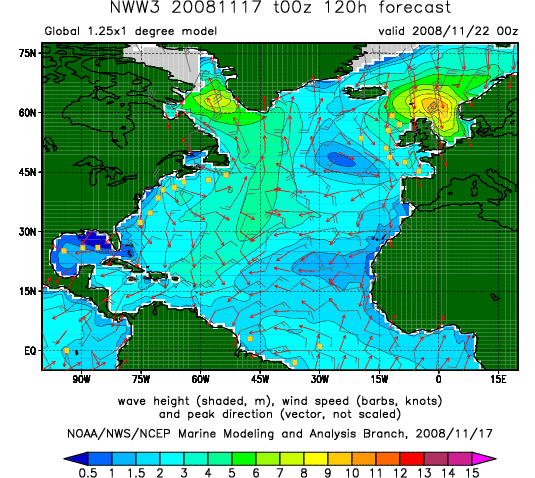
\includegraphics[width=\textwidth]{bilder/wave-watch}
    \caption{Plot einiger Elemente des Wave Watch III Modells}
    \label{wave-watch-grads}
  \end{center}
\end{figure}

\section{Verbesserung der Vorhersagen}
Die aus dem \textit{Global Forecast System} und dem \textit{Wave Watch
  III} Modell stammenden Wetter- und Wellenvorhersagen beruhen zwar
auf einem numerisch berechneten Wettermodell, können aber nur bedingt
zur Vorhersage der tatsächlichen Surfbedingungen verwendet werden. In
Kombination mit Erfahrungswerten und der Kenntnis lokaler
Gegebenheiten dienen sie eher als Indikator zur Einschätzung dieser
Bedingungen. In welcher Verbindung die Vorhersagewerte mit der
Qualität der vor Ort brechenden Wellen stehen ist unklar und variiert
wohl von Spot zu Spot. Hinzu kommt, dass wegen der groben
Gitterauflösung der Modelle die Vorhersagewerte teilweise aus der
näheren Umgebung eines Spots herangezogen werden müssen. Trotzdem sind
aber vor allem die Wellenhöhe, die Wellenperiode, die Windstärke und
die Windrichtung der Modelle wichtige Indizien, die bei der
Einschätzung der Surfbedingungen eine große Rolle spielen. Was noch
fehlt, ist eine Komponente mit der die lokalen Gegebenheiten eines
Surfspots mit ins Spiel gebracht werden. Außerdem wäre es
wünschenswert, eine Aussage über die Qualität der Surfbedingungen an
einem Spot treffen zu können.

\subsubsection{Beobachtung lokaler Gegebenheiten}
Würde man die Qualität der Surfbedingungen an einem Spot mit den dort
prognostizierten Wetter- und Wellenvorhersagen über einen längeren
Zeitraum hinweg vergleichen, könnte man wahrscheinlich bestimmte
Zusammenhänge feststellen. Beispielsweise ist es durchaus üblich, dass
zwei benachbarte Spots sehr ähnlichen Wetter- und Wellenverhältnissen
ausgesetzt sind, die Qualität der brechenden Wellen sich aber
erheblich unterscheidet. Dies kann z.B. daran liegen, dass der eine
Spot besser bei Flut und der andere besser bei Ebbe bricht. Manche
Spots wiederum fangen erst bei einer bestimmten Wellenhöhe an zu
brechen, andere hingegen sind bei zu großen Wellen nicht mehr surfbar,
da die Wellen sofort in sich zusammenfallen. Vor Ort ansässige Surfer,
sogenannte \textit{Locals}, haben oft ein feines Gespür für diese
Zusammenhänge, was wohl auf deren langjährige Beobachtungen
zurückzuführen ist.

Diese Beobachtungen von den Benutzern der Web-Applikation vornehmen zu
lassen, ist eher unrealistisch. Zum einen sind solche Beobachtungen
sehr aufwändig, und zum anderen müsste sichergestellt sein, dass diese
diszipliniert und nach denselben Kriterien durchgeführt werden. Zudem
stellt sich die Frage, wie diese Beobachtungen maschinell verwertet
und in Verbindung mit den Vorhersagen gebracht werden können.

\subsubsection{Abstimmung durch die Benutzer}
Eine im Rahmen dieser Arbeit leider nicht weiter verfolgbare Idee,
welche diese Problematik vielleicht lösen könnte, wäre die Einführung
eines Abstimmungssystems in Kombination mit
\textit{Data-Mining}-Verfahren. Informiert sich ein Benutzer auf der
Community Plattform über die Surfbedingungen an einem bestimmten Spot,
könnte man ihn zu den Bedingungen in den letzten Tagen befragen. Mit
etwas Glück kann es nämlich durchaus sein, dass der Benutzer dort
surfen war und eine Aussage über die damalige Qualität der Wellen
treffen kann. Diese Befragung sollte benutzerfreundlich und schnell
vonstatten gehen, damit sich die Besucher nicht belästigt fühlen,
sondern konstruktiv daran teilnehmen. Hier würde sich z.B. eine
Bewertungsskala von 1 bis 5 ''Sternen'' mit einer Auswahl des
entsprechenden Zeitpunktes anbieten. Die so erhobenen Datensätze
sollten Informationen über den Spot, den Zeitpunkt zu dem der Benutzer
surfen war, die Qualität der Wellen und den Benutzer selbst (optional)
enthalten. Sammelt man viele dieser Bewertungen können diese
statistisch ausgewertet und eine Aussage darüber getroffen werden, wie
gut die Surfbedingungen in der Vergangenheit waren. Mit diesen
Informationen könnte man z.B. die besten Spots in einer Region
bestimmen oder die Konsistenz der Surfbedingungen an einem Spot
ermitteln. Eine weitaus interessantere Verwendung dieser Daten wäre
aber, sie für die Bewertung von zukünftigen Surfbedingungen
einzusetzen.

\subsubsection{Bewertung zukünftiger Surfbedingungen}
Es wäre wünschenswert, wenn man einem Benutzer neben den Wetter- und
Wellenvorhersagen auch noch eine Einschätzung zur Qualität der
Surfbedingungen geben könnte, in der die lokalen Gegebenheiten eines
Spots mit berücksichtigt sind. Diese Einschätzung sollte dem Benutzer
in der ihm bekannten Bewertungsskala aus dem Abstimmungssystem
präsentiert werden. Je besser die Surfbedingungen, desto mehr
''Sterne''. Der zugrunde liegende Ansatz besteht in der Vermutung,
dass ähnliche Wetter- und Wellenvorhersagen auch ähnliche
Surfbedingungen provozieren. Wurden für einen Zeitpunkt in der
Vergangenheit positive Bewertung abgegeben, sind die Surfbedingungen
zu einem zukünftigen Zeitpunkt mit ähnlichen Wetter- und
Wellenverhältnissen vielleicht auch gut, und umgekehrt. Durch den
Vergleich historischer Vorhersagedaten mit zukünftigen, und einer
Strategie aus den abgegebenen Bewertungen, welche für die Zukunft
abzuleiten, könnte man dem Nutzer Aussagen zur Qualität zukünftiger
Surfbedingungen anbieten.

\subsubsection{Bewertungen als Klassifikationsproblem}
Die hier zu lösende Aufgabe ist ein sogenanntes
Klassifikationsproblem. Objekte einer Menge, deren
Klassenzugehörigkeit nicht bekannt ist, müssen dabei einer bestimmten
Klasse zugeordnet werden. Als Klassifikator bezeichnet man den
Algorithmus oder das Verfahren, nach dem diese Zuordnung durchgeführt
wird. Klassen würden hier durch die in mehrere Abschnitte unterteilte
Bewertungsskala repräsentiert, Objekte durch die Vorhersagen an den
Spots. Die Bewertung der Surfbedingungen würde sich dann aus der
Klasse ergeben, der eine Vorhersage zugeordnet wurde. Wüsste man, wie
sich die Variablen einer Vorhersage auf die Qualität der Wellen
auswirken, könnte man für jeden Spot einen Klassifikator konstruieren,
der idealerweise auch noch die lokalen Gegebenheiten mit
einbezieht. Die Vorschriften, wie solch ein Klassifikator jedoch
konstruiert wird, sind jedoch meistens nicht bekannt bzw. nur mit
hohem Aufwand zu ermitteln.

\subsubsection{Anwendung von Data-Mining-Verfahren}
Unter \textit{Data Mining} versteht man die Anwendung verschiedenster
Algorithmen auf einem Datenbestand, mit dem Ziel meist noch nicht
bekannte Muster zu entdecken. Neben vielen Anwendungsbeispielen ist in
\cite{Seagaran2007} nicht nur eine Zusammenfassung der in diesem
Gebiet häufig verwendeten Algorithmen zu finden, sondern auch eine
Diskussion über deren Vor- und Nachteile. Einige der dort
vorgestellten Algorithmen können dazu benutzt werden,
Klassifikationsprobleme zu lösen und bedienen sich Techniken aus dem
Bereich des maschinellen Lernens. Mit diesen Verfahren könnte versucht
werden die Zusammenhänge zwischen den Vorhersagen, den lokalen
Gegebenheiten und der Qualität der Surfbedingungen zu finden und
daraus zukünftige Bewertungen abzuleiten. \textit{Bayesian
  Classifier}, \textit{Decision Trees}, und \textit{Neuronale
  Netzwerke} sind nur einige der dort vorgestellten Algorithmen, mit
denen man versuchen könnte, dieses Problem zu lösen.

\subsubsection{Supervised Learning}
Bei Algorithmen aus dem Bereich des maschinellen Lernens unterscheidet
man zwischen Verfahren des \textit{Supervised-} und
\textit{Unsupervised Learning}. Beim \textit{Supervised Learning}
werden sogenannte Trainingsdaten benötigt, die von den Algorithmen
analysiert und zur Lösung des Problems herangezogen werden. Die
Trainingsdaten für Klassifikationsprobleme bestehen dabei aus einer
Menge von Objekten, deren Klassenzugehörigkeit bekannt ist. Die zuvor
durch ein Abstimmungssystem erhobenen Daten können nicht nur für
statistische Zwecke verwendet werden, sondern würden sich auch als
Trainingsdaten für diese Art von Algorithmen anbieten. Die
Vorhersagedaten wären dabei die Attribute eines Objekts, und die
Klassenzugehörigkeit des Objekts ist durch die Bewertung des Benutzers
festgelegt.

\subsubsection{Support Vector Machine}
Der unter dem Namen \textit{Support Vector Machine} bekannte
Algorithmus scheint ein viel versprechender Kandidat zu sein, um das
hier beschriebene Klassifikationsproblem zu lösen. Zum einen ist der
Algorithmus bei der Klassifikation von Objekten sehr schnell, und zum
anderen liefert er auch bei einer hohen Anzahl von Dimensionen recht
zuverlässige Ergebnisse. Als Dimension bezeichnet man die Attribute
eines zu klassifizierenden Objekts. Bei dem hier zu lösenden Problem
wären dies die Elemente einer Vorhersage und evtl. weitere bekannte
Eigenschaften eines Spots, die sich auf die Qualität der
Surfbedingungen auswirken könnten.

Um nun die Bewertungen zur Qualität der Surfbedingungen zu berechnen,
würde man für jeden Spot eine separate Instanz des Algorithmus
erzeugen und diese mit den bereits abgegebenen Bewertungen aus der
Vergangenheit trainieren. Jede Instanz wird dabei nur mit denjenigen
Vorhersagedaten und Bewertungen trainiert, die auch zu dem
entsprechenden Spot gehören. Je mehr Trainingsdaten vorhanden sind,
desto besser sind die Ergebnisse einer solchen Instanz. Da die
Trainingsphase aufwändiger als die eigentliche Klassifikation ist und
bei hinzukommenden Trainingsdaten die Instanz erneut mit allen
Trainingsdaten initialisiert werden muss, bieten die meisten
Implementierungen des Algorithmus die Möglichkeit, das Ergebnis der
Trainingsphase in einem sogenannten Modell zu speichern und wieder zu
laden.

Zur Berechnung einer Bewertung wird eine Vorhersage der entsprechenden
Instanz des Algorithmus übergeben, der dann das Ergebnis unter
Berücksichtigung der Trainingsdaten berechnet. Um dies Berechnung in
die Web-Applikation zu integrieren würde man beispielsweise einmal
täglich für jeden Spot eine Instanz des Algorithmus mit den
zugehörigen Trainingsdaten initialisieren und abspeichern. Da die
Klassifikation einer Vorhersage schnell zu berechnen ist, könnte die
Bewertung sogar bei einem Seitenaufruf der Web-Applikation dynamisch
generiert werden. Alternativ könnte man die Berechnung auch in den
\textit{ETL-}Prozess integrieren und alle Bewertungen in der Datenbank
vorhalten.

Anzumerken ist hier noch, dass der \textit{Support Vector Machine}
Algorithmus ein sogenanntes \textit{Black-Box} Verfahren
\cite{Seagaran2007}[S.292] ist, d.h. die lokalen Gegebenheiten eines
Spots fließen hier indirekt über die erhobenen Abstimmungsdaten mit in
die Bewertung ein. Welche Zusammenhänge allerdings zwischen den
Vorhersagedaten und den lokalen Gegebenheiten bestehen, können mit
diesem Verfahren nicht ermittelt werden.

\subsubsection{Erfolgsaussichten und Hindernisse}
Damit mit dem Algorithmus gute Ergebnisse erzielt werden, benötigt man
allerdings eine größere Menge an Trainingsdaten. Da diese zum jetzigen
Zeitpunkt nicht vorhanden sind, kann dieser Ansatz hier leider nicht
weiter verfolgt werden. Diese müssten im produktiven Betrieb der Web
Applikation über einen längeren Zeitraum durch die Benutzer erstellt
werden.

Ob dieses Verfahren überhaupt zum Ziel führt, müsste durch eine
Auswertung der Ergebnisse an verschiedenen Spots überprüft
werden. Außerdem werden dem Algorithmus bei der Initialisierung noch
einige Parameter übergeben, die sich auf die Berechnung der
Bewertungen auswirken. Diese Parameter variieren von Problem zu
Problem, können aber durch ein Verfahren das sich
\textit{Crossvalidation} nennt ermittelt werden. Eine ausführliche
Auswertung und Probephase ist deshalb auf jeden Fall erforderlich, um
die Erfolgsaussichten einschätzen zu können. Falls die Ergebnisse
einer solchen Auswertung jedoch positiv ausfallen, hätte man einen Weg
gefunden, die lokalen Gegebenheiten eines Spots indirekt über die
Trainingsdaten in Form einer Bewertung in die Vorhersagen mit
einfließen zu lassen.

%%% Local Variables:
%%% mode: latex
%%% TeX-master: "../community-plattform"
%%% End:


\bibliographystyle{geralpha}
\bibliography{literatur}

\end{document}